\documentclass[12pt,a4paper,BCOR4mm]{grsthesis}

\graphicspath{{img/}}

\usepackage[UKenglish]{babel}
\usepackage{graphicx}
\usepackage{listings}
\usepackage{amsmath}
\usepackage{array}
\usepackage{caption}
\usepackage{subfig}
\usepackage{tikz,fp}
\usepackage{braket}
\usepackage{algorithm}
\usepackage[noend]{algpseudocode}
\usepackage{longtable}
\usepackage{mathtools}
\usepackage{blkarray}
\usepackage{hyperref}
\usepackage[pagestyles, explicit, rm, bf]{titlesec}
\usepackage{titletoc}

\usetikzlibrary{shapes,arrows}

% Margins
\topmargin = -0.45in
\evensidemargin = 0in
\oddsidemargin = 0in
\textwidth = 6.3in
\textheight = 9.0in
\headsep = 0.25in
\parindent = 0in
\parskip = 0.1in
\makeatletter
\renewcommand{\@makefntext}[1]{%
  \parindent 1em%
  \normalfont$^{\@thefnmark}$#1
}
\makeatother

% Page head line
\renewpagestyle{plain}{
\headrule
\sethead[\textbf\usepage][][\hfill\textbf\chaptertitle]
{\textbf\sectiontitle}{}{\textbf\usepage}}
\renewcommand{\chapterpagestyle}{empty}

% Table of contents format
\titlecontents{chapter}[3.0em]{\addvspace{1.0pc}\large\bf} {\contentslabel{2.0em}}{\hspace*{-2.0em}}{\titlerule*[1pc]{.}\contentspage}
\titlecontents{section}[5.0em]{\addvspace{0.3pc}} {\contentslabel{2.0em}}{\hspace*{-2.0em}}{\titlerule*[1pc]{.}\contentspage}

% Numbering format
\numberwithin{equation}{chapter}
\numberwithin{figure}{chapter}
\numberwithin{table}{chapter}
\numberwithin{algorithm}{chapter}
\makeatletter
\@addtoreset{footnote}{chapter}
\makeatother

% Bold vectors
\renewcommand{\vec}[1]{\mathbf{#1}}

% Complex conjugate
\newcommand{\conj}[1]{\overline{#1}}

\begin{document}

\frontmatter{}

\maketitle
\pagestyle{empty}
\vspace*{\fill}
Copyright \copyright \; \theyear \; \theauthor

\chapter*{Abstract}

The goal of this thesis is to develop a simulation tool for the calculation
and visualization of the multiplet structure of all atoms across the periodic
table. The starting point are self-consistent calculations in the spherical-potential
approximation. For the resulting atomic levels we calculate the ab-initio
Slater parameters that define the electron-electron repulsion term of the
many-body Hamiltonian. We then construct the eigen-states of the Hamiltonian
on an open shell by constructing the multiplet states using the angular momentum
ladder operators and, where necessary, seniority. Finally, we include spin-orbit
coupling, using the ab-initio coupling constants determined from the self-consistent
radial potentials.


\pagestyle{plain}
\tableofcontents

\mainmatter{}

\chapter{Introduction}

\section{Many-body problem in quantum mechanics}
Imagine our solar system: it consists of a heavy sun with eight planets
orbiting around. In classical mechanics, the goal is to calculate the
position of each celestial object as a function of time. The motion of
the system is governed by Newton's second law: $\vec{F}=m\vec{a}$. While it is almost
impossible to solve the classical many-body problem analytically, the numerical
approach is rather straightforward. However, in quantum mechanics,
the many-body problem is a completely different story.

Scaling down to $10^{-10}$ meters, it is even philosophically profound that we
find similar structures in atomic systems as in our cosmic systems. An atom,
which consists of a heavy nucleus, with electric charge $Ze$, is surrounded by
$N$ electrons with charge $-e$. The system here is no longer governed by
Newton's second law, neither is our goal to compute the ``position'' of each
electron as a function of time. In quantum mechanics, the position of an
electron is no longer well defined. Instead, what we are looking for is the
electrons' wave function $\Psi(\vec{r}_1,\vec{r}_2,\ldots,\vec{r}_N)$ which
is the solution of the Schr\"{o}dinger equation\footnote{Strictly speaking,
Eqn.~(\ref{eq:Schr}) is called the time-independent Schr\"{o}dinger equation
and the solution $\Psi(\vec{r}_1,\vec{r}_2,\ldots,\vec{r}_N)$ is the
time-independent part of the wave function.}
\begin{equation} \label{eq:Schr}
H \Psi = E \Psi
\end{equation}
where $H$, the Hamiltonian of the system, is given by
\begin{equation} \label{eq:Hamit}
H = \sum_{i=1}^N \left[ -\frac{\hbar^2}{2m_e} \nabla_i^2 - \frac{1}{4\pi\epsilon_0} \frac{Ze^2}{r_i} \right] + \sum_{i<j}^N \frac{1}{4\pi\epsilon_0} \frac{e^2}{|\vec{r}_i - \vec{r}_j|}
\end{equation}
The term in the first sum represents the kinetic plus potential energy of the
$i$th electron, in the electric field of the nucleus. The last term, which
complicates the behavior of the system, describes the electron-electron
repulsions among all $N$ electrons (the constraint $i<j$ avoids double counting
over electron pairs).

In neither classical nor quantum mechanics, can one solve many-body problems
exactly. But in quantum mechanics, even a numerical solution is extremely
difficult to obtain. The difficulty comes from the fact that
a many-body wave function $\Psi(\vec{r}_1,\vec{r}_2,\ldots,\vec{r}_N)$ is
an object with dimension $3N$. One must generate a mesh grid with $3N$-dimension
to represent the wave function numerically and such a gigantic data is not
possible to be stored on an ordinary hard disk. Consequently, different methods
have been developed to simplify the problem and to treat the system approximately.

\section{Atomic units}
Since we are going to solve our problems numerically, it is
useful to pay attention to the choice of units. Certainly, we can use SI units,
but the scales would be inconvenient. For example, in SI units, the reduced
Planck constant reads $\hbar=1.054572\times10^{-34} \mathrm{J \cdot s}$, which
is a crazy number from a computational point of view. Hence, we employ atomic
units (a.u.), namely,
\begin{alignat*}{3}
& \text{Length:}\quad && 1\;\mathrm{a_0} && \approx 5.2918\times10^{-11}\;\mathrm{m}  \\
& \text{Mass:}\quad   && 1\;\mathrm{m_e} && \approx 9.1095\times10^{-31}\;\mathrm{kg} \\
& \text{Time:}\quad   && 1\;\mathrm{t_0} && \approx 2.4189\times10^{-17}\;\mathrm{s}  \\
& \text{Charge:}\quad && 1\;\mathrm{e}   && \approx 1.6022\times10^{-19}\;\mathrm{C}
\end{alignat*}
which are deliberately chosen such that
\begin{align}
\begin{split}
\hbar          & = 1\;\mathrm{a_0^2 m_e t_0^{-1}} \\
m_e            & = 1\;\mathrm{m_e} \\
e              & = 1\;\mathrm{e} \\
4\pi\epsilon_0 & = 1\;\mathrm{a_0^{-3} m_e t_0^2 e^2}
\end{split}
\end{align}
By adopting atomic units, the Hamiltonian in Eqn.~(\ref{eq:Hamit}) simplifies to
\begin{equation} \label{eq:HamitSimp}
H = \sum_{i=1}^N \left[ -\frac{1}{2} \nabla_i^2 - \frac{Z}{r_i} \right] + \sum_{i<j}^N \frac{1}{|\vec{r}_i - \vec{r}_j|}
\end{equation}
With the choice of atomic units, distances are given in units of the
Bohr radius ($\mathrm{a_0}$) and energies in Hartree ($\mathrm{a_0^2 m_e t_0^{-2}}$)
\begin{equation} \label{eq:EHartree}
  1\;\mathrm{Hartree}
= 2\;\mathrm{Rydberg}
\approx 27.2114\;\mathrm{eV}
\approx 4.3597\times10^{-18}\;\mathrm{J}
\end{equation}
From now on, we will keep using atomic units to simplify our equations and discussions.

\section{Convention of notations}
I will try to make the notations in my thesis as consistent as possible
to avoid confusions and to make the discussion clear.

For a many-electron wave function, we use capital psi
\begin{equation*}
\Psi(\vec{r}_1,\vec{r}_2,\ldots,\vec{r}_N)
\end{equation*}
For a one-electron wave function, we use lower case phi
\begin{equation*}
\varphi(\vec{r})
\end{equation*}
%
For a Slater determinant, we use upper case phi
\begin{equation*}
\Phi_{\alpha_1\alpha_2\cdots\alpha_N}(\vec{r}_1,\vec{r}_2,\ldots,\vec{r}_N)
\end{equation*}
%
Slater determinants are constructed from one-electron wave functions. They
are basis functions of anti-symmetric many-electron wave functions.
\begin{equation} \label{eq:introSD}
\Phi_{\alpha_1\cdots\alpha_N}(\vec{r}_1,\ldots,\vec{r}_N) = \frac{1}{\sqrt{N!}}
\begin{vmatrix}
\varphi_{\alpha_1}(\vec{r}_1) & \varphi_{\alpha_2}(\vec{r}_1) & \cdots & \varphi_{\alpha_N}(\vec{r}_1) \\
\varphi_{\alpha_1}(\vec{r}_2) & \varphi_{\alpha_2}(\vec{r}_2) & \cdots & \varphi_{\alpha_N}(\vec{r}_2) \\
\vdots & \vdots & \ddots & \vdots \\
\varphi_{\alpha_1}(\vec{r}_N) & \varphi_{\alpha_2}(\vec{r}_N) & \cdots & \varphi_{\alpha_N}(\vec{r}_N)
\end{vmatrix}
\end{equation}
%
Sometimes you hear people say, ``A many-electron wave function is a Slater determinant.''
That is wrong. A many-electron wave function is in general a linear combination of
Slater determinants, not just one (although it could be).
Nevertheless, this real-space representation of Slater determinant
in Eqn.~(\ref{eq:introSD}) will not appear in our discussion
(it only appears in Appendix~\ref{app:B}). Slater determinants will
be represented in the form of second quantization\footnote{Second quantization is
a very convenient ``algebra'' for handling many-body states. A brief discussion
of second quantization is given in Appendix~\ref{app:B}.} when later we
construct our multiplet states.




\chapter{The shooting and matching methods}

\section{The one-electron problem}
To start with, we consider the simplest case: the one-electron or hydrogen-like
system. For $N=1$, Eqn.~(\ref{eq:Schr}) (in a.u.) reads
\begin{equation} \label{eq:SchrOne}
\left[ -\frac{1}{2} \nabla^2 + V(r) \right] \varphi = E \varphi
\end{equation}
where $V(r)$ is a spherically symmetric potential (for one-electron case: $V(r)=-Z/r$).
In spherical coordinates, by separation of variables
$\varphi(r,\theta,\phi) = R(r)Y(\theta,\phi)$, Eqn.~(\ref{eq:SchrOne}) splits
into two equations, namely,
\begin{alignat}{3}
& \text{Radial equation:} \quad & \frac{d}{d r} \left( r^2 \frac{d R}{d r} \right) - 2 r^2 \left[ V(r) - E \right] R                                                                                                     & = \phantom{-}l(l+1) R \label{eq:REqn} \\
& \text{Angular equation:}\quad & \frac{1}{\sin{\theta}} \frac{\partial}{\partial \theta} \left( \sin{\theta} \frac{\partial Y}{\partial \theta} \right) + \frac{1}{\sin^2{\theta}} \frac{\partial^2 Y}{\partial \phi^2} & = -l(l+1) Y \label{eq:YEqn}
\end{alignat}
where $l$ is a non-negative integer\footnote{In fact, from the separation of variables,
there is no evidence that $l$ should be an integer. $l$ could be
any complex number. However, the boundary condition $Y(\theta,\phi)=Y(\theta,\phi+2\pi)$
and the properties of the Legendre polynomial require that $l$ must be
a non-negative integer.} known as the orbital angular momentum quantum number.
Now, a three dimensional ordinary differential equation is separated into two
equations. They are called radial equation and angular equation because
Eqn.~(\ref{eq:REqn}) has only the dependence on the radial coordinate $r$ and
Eqn.~(\ref{eq:YEqn}) has only the dependence on the angular coordinate $\theta$
and $\phi$. It is very important to realize that Eqn.~(\ref{eq:YEqn}) has
no dependence on the potential $V(r)$. Hence Eqn.~(\ref{eq:YEqn}) is
universal for all spherically symmetric potentials and its analytical solutions
are the well known spherical harmonics \cite{QM}. In other words, there is no
need to worry about Eqn.~(\ref{eq:YEqn}) since its solutions, the spherical harmonics
$Y_{lm}(\theta,\phi)$ (with $l=0,\ 1,\ \ldots$ and $m=-l,\ \ldots,\ l$),
are known exactly (see Table~\ref{table:Ylm}).
The more difficult task for us is to solve Eqn.~(\ref{eq:REqn}).
In fact, for this simplest one-electron system, the radial part solutions are also known
analytically. As a reference, Table~\ref{table:unl} lists the first few radial wave functions
for hydrogen-like atoms. A rescaled coordinate $\rho=Zr$ is used in the expressions.
Nevertheless, we are going to solve the radial equation numerically
so that we can further deal with the more general case, the many-electron system.

Eqn.~(\ref{eq:REqn}) simplifies if we change variables $u(r) \equiv rR(r)$. The
radial equation becomes
\begin{equation} \label{eq:oneElec}
\boxed{-\frac{1}{2} \frac{d^2u}{dr^2} + \left[ V(r) + \frac{l(l+1)}{2r^2} \right] u = E u}
\end{equation}
with boundary conditions: $u(r) \propto r^{l+1}$ as $r\rightarrow0$ and
$u(r) \propto \exp{(-\sqrt{-2E}r)}$ as
$r\rightarrow\infty$.

Eqn.~(\ref{eq:oneElec}) is identical in form to the one-dimensional
Schr{\"o}dinger equation, except that we have an extra ``centrifugal'' term
$[l(l+1)/2r^2]$ in addition to the external potential. Our task
is to solve this equation for $u(r)$ and determine the allowed
energies $E$.

\begin{table}[h!]
\caption{The first few analytical radial wave functions
$u_{nl}(r)$ for hydrogen-like atoms with eigen-energies $E_n=-\frac{Z^2}{2n^2}$ (Hartree).
A rescaled coordinate $\rho=Zr$ is used to simplify the expressions
and the radial coordinates $r$ are in units of Bohr radius (a.u.).}
\label{table:unl}
\begin{equation*}
\renewcommand\arraystretch{1.8}
\begin{array}{|>{\displaystyle}r >{\displaystyle}r >{\displaystyle}l >{\displaystyle}l >{\displaystyle}l|}
  \hline
  u_{10} = & 2                           & \sqrt{Z}\rho   &                                                                   & \exp{(-\rho)}   \\[0.5em] \hline
  u_{20} = & \frac{1}{\sqrt{2}}          & \sqrt{Z}\rho   & \Big(1-\frac{1}{2}\rho\Big)                                       & \exp{(-\rho/2)} \\
  u_{21} = & \frac{1}{\sqrt{24}}         & \sqrt{Z}\rho^2 &                                                                   & \exp{(-\rho/2)} \\[0.5em] \hline
  u_{30} = & \frac{2}{\sqrt{27}}         & \sqrt{Z}\rho   & \Big(1-\frac{2}{3}\rho+\frac{2}{27}\rho^2\Big)                    & \exp{(-\rho/3)} \\
  u_{31} = & \frac{8}{27\sqrt{6}}        & \sqrt{Z}\rho^2 & \Big(1-\frac{1}{6}\rho\Big)                                       & \exp{(-\rho/3)} \\
  u_{32} = & \frac{4}{81\sqrt{30}}       & \sqrt{Z}\rho^3 &                                                                   & \exp{(-\rho/3)} \\[0.5em] \hline
  u_{40} = & \frac{1}{4}                 & \sqrt{Z}\rho   & \Big(1-\frac{3}{4}\rho+\frac{1}{8}\rho^2-\frac{1}{192}\rho^3\Big) & \exp{(-\rho/4)} \\
  u_{41} = & \frac{\sqrt{5}}{16\sqrt{3}} & \sqrt{Z}\rho^2 & \Big(1-\frac{1}{4}\rho+\frac{1}{80}\rho^2\Big)                    & \exp{(-\rho/4)} \\
  u_{42} = & \frac{1}{64\sqrt{5}}        & \sqrt{Z}\rho^3 & \Big(1-\frac{1}{12}\rho\Big)                                      & \exp{(-\rho/4)} \\
  u_{43} = & \frac{1}{768\sqrt{35}}      & \sqrt{Z}\rho^4 &                                                                   & \exp{(-\rho/4)} \\[0.5em]
  \hline
\end{array}
\end{equation*}
\end{table}

\section{Logarithmic grid}
We are now in a position to solve the one-dimensional ordinary differential
equation in (\ref{eq:oneElec}) numerically. It is often convenient to solve
problems on uniform grids. However, the curvature\footnote{The second derivative
$u'' = -2[E-V(r)-l(l+1)/2r^2]u$.} of the wave function
indicates that the function $u(r)$ oscillates faster if $r$ goes smaller.
This suggests us to take more points for small $r$ but fewer for large $r$.
For instance, Fig.~\ref{fig:hydrlike} plots the exact wave functions from Table~\ref{table:unl} with
principal quantum number $n=4$ for three hydrogen-like atoms. These plots demonstrate
that the smaller $r$ goes, the stronger is the oscillation of the function $u(r)$.
And the wave functions are attracted more closely to the nucleus with increasing
nuclear charge $Z$. Many grid points will be wasted to sample the non-fruitful outer
regions where the wave function is almost zero (see Fig.~\ref{fig:Z3}). Therefore, an
adaptive grid with higher resolution close to the nucleus is desired.

\begin{figure}[h!]
\centering
\subfloat[][$Z=1$]{\includegraphics[width=0.325\textwidth]{Z1}\label{fig:Z1}}
\subfloat[][$Z=2$]{\includegraphics[width=0.325\textwidth]{Z2}\label{fig:Z2}}
\subfloat[][$Z=3$]{\includegraphics[width=0.325\textwidth]{Z3}\label{fig:Z3}}
\caption{Plots of exact solutions for a few hydrogen-like wave functions with
principal quantum number $n=4$. (a) wave functions of $Z=1$; (b) wave functions of $Z=2$;
(c) wave functions of $Z=3$. The plots demonstrate the smaller $r$ goes,
the stronger is the oscillation of the function $u(r)$. And the wave functions
are attracted more closely to the nucleus with increasing nuclear charge $Z$.}
\label{fig:hydrlike}
\end{figure}

Our choice is to use a logarithmic grid\footnote{The logarithmic grid is not
the unique choice. One can use any adaptive grid as long as it can
properly represent the wave function. But the logarithmic grid uses a change of
variable technique and it is very elegant.} \cite{ES},
$ 0 < r_0 < r_1 < \cdots < r_{n-1} < \infty $, where
\begin{equation} \label{eq:x2r}
r_i = \frac{1}{Z} e^{x_i} \quad\text{or equivalently}\quad \rho_i=e^{x_i}
\end{equation}
\begin{center}
\setlength{\unitlength}{5pt}
\begin{picture}(53.6518,0)
\put(0,0){\line(1,0){53.6518}}
\put(0,0){\line(0,1){1}}
\put(0.2216,0){\line(0,1){1}}
\put(0.4923,0){\line(0,1){1}}
\put(0.8229,0){\line(0,1){1}}
\put(1.2268,0){\line(0,1){1}}
\put(1.7200,0){\line(0,1){1}}
\put(2.3224,0){\line(0,1){1}}
\put(3.0583,0){\line(0,1){1}}
\put(3.9570,0){\line(0,1){1}}
\put(5.0547,0){\line(0,1){1}}
\put(6.3954,0){\line(0,1){1}}
\put(8.0330,0){\line(0,1){1}}
\put(10.0332,0){\line(0,1){1}}
\put(12.4762,0){\line(0,1){1}}
\put(15.4601,0){\line(0,1){1}}
\put(19.1046,0){\line(0,1){1}}
\put(23.5561,0){\line(0,1){1}}
\put(28.9931,0){\line(0,1){1}}
\put(35.6339,0){\line(0,1){1}}
\put(43.7449,0){\line(0,1){1}}
\put(53.6518,0){\line(0,1){1}}
\put(-0.5,-2){$r_0$}
\put(53.1518,-2){$r_{n-1}$}
\end{picture}
\end{center}
and $x$ is a uniformly distributed grid
\begin{equation} \label{eq:xDis}
x_i = x_0 + i \Delta x
\end{equation}
\begin{center}
\setlength{\unitlength}{5pt}
\begin{picture}(53.6520,0)
\put(0,0){\line(1,0){53.6520}}
\put(0,0){\line(0,1){1}}
\put(2.6826,0){\line(0,1){1}}
\put(5.3652,0){\line(0,1){1}}
\put(8.0478,0){\line(0,1){1}}
\put(10.7304,0){\line(0,1){1}}
\put(13.4130,0){\line(0,1){1}}
\put(16.0956,0){\line(0,1){1}}
\put(18.7782,0){\line(0,1){1}}
\put(21.4608,0){\line(0,1){1}}
\put(24.1434,0){\line(0,1){1}}
\put(26.8260,0){\line(0,1){1}}
\put(29.5086,0){\line(0,1){1}}
\put(32.1912,0){\line(0,1){1}}
\put(34.8738,0){\line(0,1){1}}
\put(37.5564,0){\line(0,1){1}}
\put(40.2390,0){\line(0,1){1}}
\put(42.9216,0){\line(0,1){1}}
\put(45.6042,0){\line(0,1){1}}
\put(48.2868,0){\line(0,1){1}}
\put(50.9694,0){\line(0,1){1}}
\put(53.6520,0){\line(0,1){1}}
\put(-0.5,-2){$x_0$}
\put(53.1520,-2){$x_{n-1}$}
\end{picture}
\end{center}

The advantage of this logarithmic grid will be clear in a short while.
First, we introduce a rescaled quantity\footnote{Don't be confused
with the rescalings. As a remark, the relation among $R$, $u$ and $\tilde{u}$
is the following: $R(r) \equiv u(r)/r \equiv \tilde{u}(r)/\sqrt{r}$.}
$\tilde{u} \equiv u/\sqrt{r}$. Recall our analytical solutions in Table~\ref{table:unl},
now instead of $u_{nl}(r)$, we give the relations between $\tilde{u}_{nl}$ and $x$ in
Table~\ref{table:unlt}.

\begin{table}[h!]
\caption{The first few rescaled radial wave functions
$\tilde{u}_{nl}(x)$ for hydrogen-like atoms with atomic number $Z$. The
coordinates $x$ are the logarithmic transformations from the radial coordinate $r$.}
\label{table:unlt}
\begin{equation*}
\renewcommand\arraystretch{1.8}
\begin{array}{|>{\displaystyle}r >{\displaystyle}r >{\displaystyle}l >{\displaystyle}l >{\displaystyle}l|}
  \hline
  \tilde{u}_{10} = & 2                           & Ze^{x/2}  &                                                                    & \exp{(-e^{x})}   \\[0.5em] \hline
  \tilde{u}_{20} = & \frac{1}{\sqrt{2}}          & Ze^{x/2}  & \Big(1-\frac{1}{2}e^{x}\Big)                                       & \exp{(-e^{x}/2)} \\
  \tilde{u}_{21} = & \frac{1}{\sqrt{24}}         & Ze^{3x/2} &                                                                    & \exp{(-e^{x}/2)} \\[0.5em] \hline
  \tilde{u}_{30} = & \frac{2}{\sqrt{27}}         & Ze^{x/2}  & \Big(1-\frac{2}{3}e^{x}+\frac{2}{27}e^{2x}\Big)                    & \exp{(-e^{x}/3)} \\
  \tilde{u}_{31} = & \frac{8}{27\sqrt{6}}        & Ze^{3x/2} & \Big(1-\frac{1}{6}e^{x}\Big)                                       & \exp{(-e^{x}/3)} \\
  \tilde{u}_{32} = & \frac{4}{81\sqrt{30}}       & Ze^{5x/2} &                                                                    & \exp{(-e^{x}/3)} \\[0.5em] \hline
  \tilde{u}_{40} = & \frac{1}{4}                 & Ze^{x/2}  & \Big(1-\frac{3}{4}e^{x}+\frac{1}{8}e^{2x}-\frac{1}{192}e^{3x}\Big) & \exp{(-e^{x}/4)} \\
  \tilde{u}_{41} = & \frac{\sqrt{5}}{16\sqrt{3}} & Ze^{3x/2} & \Big(1-\frac{1}{4}e^{x}+\frac{1}{80}e^{2x}\Big)                    & \exp{(-e^{x}/4)} \\
  \tilde{u}_{42} = & \frac{1}{64\sqrt{5}}        & Ze^{5x/2} & \Big(1-\frac{1}{12}e^{x}\Big)                                      & \exp{(-e^{x}/4)} \\
  \tilde{u}_{43} = & \frac{1}{768\sqrt{35}}      & Ze^{7x/2} &                                                                    & \exp{(-e^{x}/4)} \\[0.5em]
  \hline
\end{array}
\end{equation*}
\end{table}

If we compare Table~\ref{table:unl} and Table~\ref{table:unlt} carefully, we can
find that in the previous formulas, the radial coordinates $r$ are always scaled by a factor
of $Z$, so are the plots in Fig.~\ref{fig:hydrlike}. But with the transformed
coordinate $x$, we no longer have this horizontal scaling and this helps us better work
with heavy nuclei. Meanwhile, the transformed coordinate $x$ ``magnifies'' the
inner region while shrinks the outer. As shown in Fig.~\ref{fig:hydrliket},
we plot the rescaled wave functions with (again) principal quantum number $n=4$
for the three hydrogen-like atoms. In contrast to Fig.~\ref{fig:hydrlike},
the three plots are identical except for a vertical scaling factor $Z$.
The inner regions are magnified clearly and the less important outer regions are reduced.
\begin{figure}[h!]
\centering
\subfloat[][$Z=1$]{\includegraphics[width=0.325\textwidth]{Z1t}\label{fig:Z1t}}
\subfloat[][$Z=2$]{\includegraphics[width=0.325\textwidth]{Z2t}\label{fig:Z2t}}
\subfloat[][$Z=3$]{\includegraphics[width=0.325\textwidth]{Z3t}\label{fig:Z3t}}
\caption{The rescaled wave functions with principal quantum number $n=4$
for three hydrogen-like atoms on the transformed grid $x$. (a) wave functions of $Z=1$;
(b) wave functions of $Z=2$; (c) wave functions of $Z=3$. The three plots are
identical except for a vertical scaling factor $Z$. The inner regions
are magnified clearly and the less important outer regions are reduced.}
\label{fig:hydrliket}
\end{figure}

The original problem $u$ on the radial coordinate $r$ can be easily transformed to the
rescaled problem $\tilde{u}$ on the transformed coordinate $x$ by the change of variable
technique. The idea is to replace the second derivative $d^2u/dr^2$ in Eqn.~(\ref{eq:oneElec})
in terms of $d^2\tilde{u}/dx^2$:
\begin{equation} \label{eq:dudx}
\frac{d^2u}{dr^2} = -\frac{1}{4}r^{-3/2} \tilde{u} + r^{-3/2} \frac{d^2 \tilde{u}}{dx^2}
\end{equation}
%
Substituting Eqn.~(\ref{eq:dudx}) into Eqn.~(\ref{eq:oneElec}), we obtain
\begin{equation} \label{eq:oneElecTrans}
-\frac{1}{2} \frac{d^2\tilde{u}}{dx^2} + \left[ r^2 V(r) + \frac{1}{2} \Big(l+\frac{1}{2}\Big)^2 \right] \tilde{u} = r^2 E \tilde{u}
\end{equation}
This is our transformed problem. Now, instead of solving
Eqn.~(\ref{eq:oneElec}) directly, we solve this
transformed equation in (\ref{eq:oneElecTrans}). This logarithmic
transformation is a key to obtaining accurate numerical solutions.

\section{Numerov's method}
The next immediate question is: how to discretize the second derivative in
Eqn.~(\ref{eq:oneElecTrans}) so that we can implement numerical integrations
in our computer program. Perhaps the simplest way is to write this second
derivative in the finite-difference form:
\begin{equation} \label{eq:FD}
\frac{d^2\tilde{u}}{dx^2} \approx \frac{\tilde{u}_{i+1} - 2\tilde{u}_i + \tilde{u}_{i-1}}{\Delta x^2}
\end{equation}
%
This discretization is perfectly valid and we can integrate
Eqn.~(\ref{eq:oneElecTrans}) numerically with 2nd order accuracy.
Nevertheless, there exists a very smart trick which allows us to obtain a 4th
order accurate solution with almost the same amount of computational effort.
This trick is called Numerov's method.

If we take a close look at Eqn.~({\ref{eq:FD}}), we get higher order terms:
\begin{equation} \label{eq:FDhigher}
\frac{d^2\tilde{u}}{dx^2} = \frac{\tilde{u}_{i+1} - 2\tilde{u}_i + \tilde{u}_{i-1}}{\Delta x^2} - \frac{1}{12}\tilde{u}_i^{(4)}\Delta x^2 + \mathcal{O}(\Delta x^4)
\end{equation}
%
But the fourth derivative $\tilde{u}_i^{(4)}$ can be also written in the
finite-difference form:
\begin{equation} \label{eq:FDhigherFD}
\frac{d^2\tilde{u}}{dx^2} = \frac{\tilde{u}_{i+1} - 2\tilde{u}_i + \tilde{u}_{i-1}}{\Delta x^2} - \frac{1}{12}\frac{\tilde{u}_{i+1}^{''} - 2\tilde{u}_i^{''} + \tilde{u}_{i-1}^{''}}{\Delta x^2}\Delta x^2 + \mathcal{O}(\Delta x^4)
\end{equation}
%
Here comes the smart trick, instead of treating the second derivative $\tilde{u}_i^{''}$ in
Eqn.~(\ref{eq:FDhigherFD}) numerically, we can simply replace the $\tilde{u}_i^{''}$
by the relation from the original ODE in (\ref{eq:oneElecTrans}):
\begin{equation} \label{eq:NmvTrick}
\tilde{u}_i^{''} = -2 k_i^2 \tilde{u_i}
\end{equation}
where,
\begin{equation} \label{eq:kk}
k_i^2 \equiv r_i^2 E - r_i^2 V(r_i) - \frac{1}{2} \Big(l+\frac{1}{2}\Big)^2
\end{equation}
%
What remains are simply substitutions. We substitute Eqn.~(\ref{eq:NmvTrick}) into
Eqn.~(\ref{eq:FDhigherFD}) and then substitute Eqn.~(\ref{eq:FDhigherFD}) into
Eqn.~(\ref{eq:oneElecTrans}), we obtain the following relation:
\begin{equation} \label{eq:Numerov}
\boxed{\tilde{u}_{i\pm1} = \frac{(2-\frac{5\Delta x^2}{3}k_i^2)\tilde{u}_i - (1+\frac{\Delta x^2}{6}k_{i\mp1}^2)\tilde{u}_{i\mp1}}{1+\frac{\Delta x^2}{6}k_{i\pm1}^2}}
\end{equation}
%
Eqn.~(\ref{eq:Numerov}) is a simple 3-point recursion: with the knowledge of
$\tilde{u}_{i-1}$ and $\tilde{u}_i$, we can compute $\tilde{u}_{i+1}$ easily
(or from the other direction: to compute $\tilde{u}_{i-1}$ from $\tilde{u}_i$
and $\tilde{u}_{i+1}$).
We are now facing two questions:
\begin{enumerate}
  \item How do we choose the ``starting points'', say, $\tilde{u}_0$
        and $\tilde{u}_1$?
  \item The parameter $k_i^2$ has a dependence on the energy $E$, which is so far
        unknown to us. How do we determine this energy?
\end{enumerate}
Keep those two questions in mind and we will discuss them in detail in the
following section.

\section{The two-sided shooting and matching}
First of all, let's define our grid on which we solve our numerical problem:
\begin{equation} \label{eq:grid}
\left\{ r_{\text{min}} = \frac{0.0001}{Z};\quad r_{\text{max}} = 50.0;\quad \Delta x = 0.002; \right\}
\end{equation}
The minimum of the radial grid $r_{\text{min}}$ depends on the atomic number $Z$,
because the higher the nuclear charge, the closer the electron wave function
will be attracted to the origin. We cannot take $r_{\text{min}}=0$
as $x_{\text{min}} = \ln{(Zr_{\text{min}})}$ will be $-\infty$. The maximum of the radial
grid is a constant $r_{\text{max}} = 50.0$. This consideration is from the fact that the size of
each atom will be roughly the same after self-consistent calculations.\footnote{The
self-consistent calculation will be discussed in a later chapter.
By saying the size of an atom, we mean the distribution range that is covered
by the significant part of the electron wave functions.} Please notice that
we define $\Delta x$ instead of $\Delta r$, because the grid $x_i$ is uniformly
spaced whereas the spacing $\Delta r$ is not a constant.\footnote{As a reference,
number of grid points $\#$: $Z=1\,\rightarrow\,\#=6563$; $Z=10\,\rightarrow\,\#=7713$;
$Z=100\,\rightarrow\,\#=8865$.}

Let's start with the first question we had in our last section: the
initialization of the wave functions. We initialize our wave functions
according to their asymptotes (referring to the boundary conditions
in Eqn.~(\ref{eq:oneElec})):
\begin{alignat}{3} \label{eq:asym}
\tilde{u}(r) & \propto r^{l+1}/\sqrt{r}          && \quad\text{as}\quad r\rightarrow0 \\
\tilde{u}(r) & \propto e^{-\beta r}/\sqrt{r} && \quad\text{as}\quad r\rightarrow\infty
\end{alignat}
%
where $\beta = \sqrt{-2E}$. We perform the numerical integrations from both the forward and the backward
directions.\footnote{One could also implement a one-sided only integration.
However, because of the numerical instability, the solution will diverge out
quickly. A two-sided integration is perhaps the best approach to minimize
the effect of numerical instability.} The corresponding initializations
are summarized in Table~\ref{table:init}.
One might worry about the sign of the energy
$E$ as a positive energy will make the square root imaginary. But we will not
work with positive energies as we are interested only in the bounded states
whose energies are always below zero. A positive energy will result in a scattering
state which is not of our concern here.
%
\begin{table}[h!]
\caption{Wave function initializations for the forward and the backward
directions.}
\label{table:init}
\begin{center}
\begin{tabular}{|c|c|}
  \hline
  & Initialization \\ \hline
  Forward &
  $\begin{aligned}
  \smash[b]{\vphantom{\Big|}}
  \tilde{u}_0 & = r_0^{l+1} / \sqrt{r_0} \\
  \tilde{u}_1 & = r_1^{l+1} / \sqrt{r_1}
  \smash[t]{\vphantom{\Big|}}
  \end{aligned}$ \\ \hline
  Backward &
  $\begin{aligned}
  \smash[b]{\vphantom{\Big|}}
  \tilde{u}_{n-1} & = e^{-\beta r_{n-1}} / \sqrt{r_{n-1}} \\
  \tilde{u}_{n-2} & = e^{-\beta r_{n-2}} / \sqrt{r_{n-2}}
  \smash[t]{\vphantom{\Big|}}
  \end{aligned}$ \\
  \hline
\end{tabular}
\end{center}
\end{table}

Be careful there is a pitfall in the backward initialization. Let's say we take
$r_{n-1} = 50$ and $E = -300$. The term $e^{-\beta r_{n-1}}$ will have
a value approximately $1.26\times10^{-532}$, which is such a small number that
cannot be represented by a double precision floating point number. As a result,
this initialization will return us $0$.
But if $\tilde{u}_{n-1}$ and $\tilde{u}_{n-2}$ are zeros, the resulting
$\tilde{u}_{n-3}$, $\tilde{u}_{n-4}$, $\ldots$ from the integration
in Eqn.~(\ref{eq:Numerov}) will all become zeros.
And of course this is not what we wanted. To overcome this problem, we should
keep doing the initialization for $\tilde{u}_{n-3}$, $\tilde{u}_{n-4}$, $\ldots$
until we meet the first $\tilde{u}_i$ which is nonzero. And this $\tilde{u}_i$
and the next $\tilde{u}_{i-1}$ will be our starting points for the backward integrations.
Actually the same argument applies to the forward initialization. If $r_0$
goes extremely small, $\tilde{u}_0$ will also have an arithmetic underflow
problem. However, unlike the exponential term in the backward initialization,
this value will not drop to zero that quickly. In our practical problems, we do
not need to worry about the underflow problems in the forward direction and can simply
assign the initial values to $\tilde{u}_0$ and $\tilde{u}_1$.

There is one important hidden message in Eqn.~(\ref{eq:Numerov}):
If any two adjacent points (not necessarily the end ones) are given,
the entire wave function can be reconstructed. This is the underlying
principle of how one should match the wave functions from the forward and
backward integrations. Ideally, if $E$ is an eigen-energy, the resulting
wave functions from the forward and backward integrations will be identical
(up to a normalization\footnote{Normalization of wave functions will be
discussed in the later section.} factor). On the other hand, if $E$ is not an
eigen-energy, the wave functions will not match. To check whether two wave functions
matched or not, we do not compare the entire wave functions (they
will never match due to numerical instability). What we should match instead
are two adjacent points on the two wave functions.
As we mentioned before, if the solutions agree in two points, in principle
they will agree everywhere. But which two points do we compare?
Apparently, those two points should not be too close to the boundaries. Because of
numerical instability, the wave functions will diverge out quickly if integrating
into classically forbidden regions. A good choice of these two points could be around
the classical turning point. A classical turning point is the position where
the energy of the electron is equal to the potential\footnote{The true classical turning
point should be at $E=V_{\text{eff}}(r)$ where $V_{\text{eff}}(r)=V(r)+\frac{l(l+1)}{2r^2}$.
But it is better to only use $V(r)$ here since $V_{\text{eff}}(r)$ will introduce an additional
root near the origin.} $E=V(r)$. Beyond the classical turning point,
the electron reaches the classically forbidden region. And inside this region,
the electron wave function will decay exponentially and no further node\footnote{A node
is a point along the wave function where the wave function goes through zero.
See Fig.~\ref{fig:hydrlike} and Fig.~\ref{fig:hydrliket} for example.} will
be created. Our matching points $r_{\text{M1}}$ and $r_{\text{M2}}$ (they are adjacent)
are taken such that $E \ge V(r_{\text{M1}})$ and $E<V(r_{\text{M2}})$ (see Fig.~\ref{fig:r1r2}).
A so called matched wave function satisfies the following criterion,
\begin{equation} \label{eq:crit}
\big|\tilde{u}_{\text{F}1} \tilde{u}_{\text{B}2} - \tilde{u}_{\text{F}2} \tilde{u}_{\text{B}1}\big| < \varepsilon
\end{equation}
where $\varepsilon$ is a small tolerance, say, $\varepsilon=10^{-8}$.
The subscripts ``F'' and ``B'' denote whether the wave function comes
form the forward integration or from the other direction. One might ask
why don't we simply compare the two points such that
$|\tilde{u}_{\text{F}1} - \tilde{u}_{\text{B}1}| < \varepsilon$
and $|\tilde{u}_{\text{F}2} - \tilde{u}_{\text{B}2}| < \varepsilon$.
But we should understand that the two wave functions from the forward and backward
directions need to match only up to a normalization factor.
The initialization in Table~\ref{table:init} does not guarantee that
the wave functions from the two directions will have the same scaling factor.
\begin{figure}[h!]
\centering
  \includegraphics[width=0.45\textwidth]{r1r2}
  \caption{Two matching points when $E=-0.4$ with potential $V(r)=-1/r$ on a sample grid.}
  \label{fig:r1r2}
\end{figure}

As an important note, instead of comparing the two points, many people would
like to compare the first derivatives of the two wave functions at a matching position.
That is also very intuitive as a matched wave function should be ``smooth''. However,
comparing the first derivatives will introduce additional numerical error unless the
derivative is calculated with a formula consistent with the Numerov's integration.
The comparison of two adjacent points does that automatically, which will give us
a 4th order accuracy that is consistent with the Numerov's method.

So, everything is ready. What remains is to determine the electron energy $E$.
Believe it or not, the determination of $E$ is a trial-and-error approach.
As demonstrated in Fig.~\ref{fig:match}, we first make a guess to the energy
$E=-0.6$. Then we perform the integration (the so called shooting) and find
out the wave functions at the matching point do not match and the guessed
energy was too low. Next we increase our energy $E=-0.4$ and realize the
energy is too high this time. Finally, by trial-and-error, we lock on the
eigen-energy which in this case should be $E=-0.5$. This trial-and-error strategy
is actually the spirit of the shooting and matching method.

\begin{figure}[h!]
\centering
\subfloat[][$E=-0.6$]{\includegraphics[width=0.325\textwidth]{E06}\label{fig:E06}}
\subfloat[][$E=-0.4$]{\includegraphics[width=0.325\textwidth]{E04}\label{fig:E04}}
\subfloat[][$E=-0.5$]{\includegraphics[width=0.325\textwidth]{E05}\label{fig:E05}}
\caption{Forward integration and backward integration matching for the wave
function $u_{10}$ of a hydrogen atom ($Z=1$). It is really a trial-and-error
strategy to determine the eigen-energy.}
\label{fig:match}
\end{figure}

\section{The bisection method}
Suppose we have our program codes ready, our next job is to modify the parameter
$E$ and run the program over and over to find out the possible eigen-energies and
the corresponding eigen-functions. This is a rather tedious job. But an experienced
programmer (like us) will soon notice that we could let the machine do this trial-and-error
process automatically.

This automation procedural is called the bisection method. The idea is to start
from two initial guesses $E_{\text{low}}$ and $E_{\text{up}}$, and locate the
solution\footnote{It is very likely that more than one eigen-states are in
between $E_{\text{low}}$ and $E_{\text{up}}$. But the algorithm for finding all of them will
be more complicated and one has to be more careful for that situation. For
simplicity, here we only provide an algorithm for locating one eigen-state.}
in between. We provide the bisection algorithm for identifying the
eigen-states in Algorithm~\ref{alg:bisect}.

\begin{algorithm}[h!]
\caption{Bisection method}\label{alg:bisect}
\begin{algorithmic}[1]
\Function{Bisection}{$E_{\text{low}}$, $E_{\text{up}}$}
\State $eigen_{\text{low}} \gets$ \Call{Shoot}{$E_{\text{low}}$}
\State $eigen_{\text{up}} \gets$ \Call{Shoot}{$E_{\text{up}}$}
\State $match_{\text{low}} \gets eigen_{\text{low}}.match$
\State $match_{\text{up}} \gets eigen_{\text{up}}.match$
\State $node_{\text{low}} \gets eigen_{\text{low}}.node$
\State $node_{\text{up}} \gets eigen_{\text{up}}.node$
\If {$node_{\text{up}}-node_{\text{low}} = 1$
{\bf and} $match_{\text{up}}*match_{\text{low}} < 0$}
\Loop
\State $E \gets (E_{\text{low}}+E_{\text{up}})/2$
\State $eigen \gets$ \Call{Shoot}{$E$}
\State $match \gets eigen.match$
\If {$|match| < \varepsilon$} \Comment {Eigen-state found}
\State \Return $eigen$
\Else
\If {$match*match_{\text{low}} > 0$}
\State $E_{\text{low}} \gets E$
\State $match_{\text{low}} \gets match$
\ElsIf {$match*match_{\text{up}} > 0$}
\State $E_{\text{up}} \gets E$
\State $match_{\text{up}} \gets match$
\Else
\State \Return false
\EndIf
\EndIf
\EndLoop
\Else
\State \Return false
\EndIf
\EndFunction
\end{algorithmic}
\end{algorithm}

The mysterious function \texttt{Shoot}() in Algorithm~\ref{alg:bisect} is
basically the initialization and Numerov integration that we discussed in
previous sections. The function \texttt{Shoot}() takes an argument $E$ and
returns an object which contains all the essential information of the resulting
wave function, including the energy, the normalized wave function, number
of nodes, the matching quality (as defined
in Eqn.~(\ref{eq:crit})), etc. The difference between the number of nodes
from $E_{\text{low}}$ and $E_{\text{up}}$ determines the number of
eigen-states between them. As a remark, there is a close relation among
the number of nodes, the principal quantum number and the orbital angular
momentum quantum number: $n = node + l + 1$.

\section{Normalizing the wave function}
In the previous sections, we mentioned the wave function normalization. By saying
normalizing a wave function, it means to find a factor $A$ such that
\begin{equation} \label{eq:norm}
A \int_0^\infty dr\,|u|^2 = 1
\end{equation}
The re-assignment $u \gets \sqrt{A}u$ normalizes the wave function.

It is now a matter of how to evaluate this integral numerically. First of all,
it would be convenient if we transform our problem onto the uniform grid $x$.
By change of variable $dr = (dr/dx)dx$, Eqn.~(\ref{eq:norm}) becomes
\begin{equation} \label{eq:normt}
A \int_0^\infty dx\,r\,|u|^2 = 1
\end{equation}
%
There are three standard numerical methods to compute the definite integrals.
The first one, which is the simplest, will be exact if the integrand $f(x)$ is
a piecewise constant function. It is called the rectangle rule.
\begin{equation} \label{eq:rect}
\int_{x_0}^{x_{n-1}} dx\,f(x) \approx \Delta x \sum_{i=0}^{n-2}{f(x_i)}
\end{equation}
%
The second one, the trapezoidal rule, will be exact if the integrand
is piecewise linear.
\begin{equation} \label{eq:tpzd}
\int_{x_0}^{x_{n-1}} dx\,f(x) \approx \frac{\Delta x}{2} \sum_{i=0}^{n-2}{\left[f(x_i) + f(x_{i+1})\right]}
\end{equation}
%
The next order is quadratic. The Simpson's rule does an interpolation on each
3-point stencil. It is exact when the integrand is piecewise quadratic.
In order to concatenate every 3-point stencil together,
it requires the total number of the grid points to be odd.
The Simpson's rule is often more accurate than the rectangle and
trapezoidal rules. Here I use $(+2)$ in the summation to denote the index $i$ jumps
in steps of 2.
\begin{equation} \label{eq:simp}
\int_{x_0}^{x_{n-1}} dx\,f(x) \approx \frac{\Delta x}{3} \left[f(x_0) + 4\sum_{i=1(+2)}^{n-2}{f(x_i)} + 2\sum_{i=2(+2)}^{n-3}{f(x_i)} + f(x_{n-1})\right]
\end{equation}
%
To compare those three methods, we calculate the numerical results
for the following sample integration (whose analytical solution can be computed easily):
\begin{equation} \label{eq:sampInt}
\int_{x_0}^{x_{n-1}} dx\,r\,\sin{(x)}
\end{equation}
on a few grids with different spacing:
\begin{equation} \label{eq:sampIntGrid}
\left\{ r_{\text{min}} = 1.0;\quad r_{\text{max}} = 50.0;\quad \Delta x = 10^0,10^{-1},\ldots,10^{-6}; \right\}
\end{equation}
%
We plot the relative error against the grid size $\Delta x$
on a log-log scale for the three methods, rectangle, trapezoidal
and Simpson. The results are shown in Fig.~\ref{fig:rts}.
In the log-log scale plot, the slope of each curve indicates the order
of accuracy of each method. Apparently, the Simpson's rule gives
the highest order among the three methods. There is a ``turning point''
on the Simpson's curve around $\Delta x = 10^{-3}$, since the solution hits
the machine precision. In our shooting method problems, we have a grid
with $\Delta x = 0.002$ and the Simpson's rule is our choice.

\begin{figure}[h!]
\centering
  \includegraphics[width=0.5\textwidth]{rts}
  \caption{Numerical integrations for $f(x)=r\sin{(x)}$ using
  rectangle, trapezoidal and Simpson's rules. This figure plots the relative
  error against the grid size $\Delta x$ on a log-log scale. 
  The slope of each curve indicates the order of the accuracy.}
  \label{fig:rts}
\end{figure}

\section{Numerical and exact eigen-energy comparison}
To confirm the correctness of our results and to check the accuracy, we can
compare our numerical solutions with the analytical eigen-energies of hydrogen-like
atoms. The eigen-energies of a hydrogen-like atom is given by (in Hartree)
\begin{equation} \label{eq:eigE}
E_n = -\frac{Z^2}{2n^2}
\end{equation}
%
We selected a few one-electron ions for comparison, namely H ($Z=1$), $\text{C}^{5+}$ ($Z=6$),
$\text{Fe}^{25+}$ ($Z=26$), $\text{Ag}^{46+}$ ($Z=47$) and $\text{U}^{91+}$ ($Z=92$).
Please notice that they are not neutral atoms, but with only one electron inside
(this is what we are able to deal with up to this stage). Table~\ref{table:eigE} lists the numerical
and exact eigen-energies for the selected elements. Energies are given in
units of Hartree (a.u.). The absolute error $e_{\text{abs}} = |E_{\text{num}} - E_{\text{exa}}|$
and the relative error $e_{\text{rel}} = |(E_{\text{num}} - E_{\text{exa}})/E_{\text{exa}}|$
are listed accordingly. The symbols in column 2 are the orbital names. For
instance, $2p$ is an orbital with principal quantum number $n=2$ and orbital angular momentum
quantum number $l=1$. A direct mapping between $l$ and its ``name'' is given below:
\begin{center}
\begin{tabular}{ c | c | c | c | c | c | c }
  \hline
  $l$          & 0 & 1 & 2 & 3 & 4 & 5 \\ \hline
  orbital name & $s$ & $p$ & $d$ & $f$ & $g$ & $h$ \\
  \hline
\end{tabular}
\end{center}

With this nicely tabulated result, we conclude our one-electron system computation
in this section. From the next chapter, we will start to work on with more
complicated, more realistic and of course more exciting cases, the many-electron systems.

\begin{table}[h!]
\caption{The numerical and exact eigen-energies for the selected
one-electron atoms. Energies are given in units of Hartree (a.u.).}
\label{table:eigE}
\begin{center}
\begin{tabular}{ c | c | r | r | r | r }
  \hline
 Elem & Orbital & Numerical & Exact & Abs Error & Rel Error \\ \hline \hline
  H &  $1s$  &  $-0.500000$  &  $-0.500000$  &  0.000000  &  0.000000 \\  \hline
  C &  $1s$  &  $-18.000002$  &  $-18.000000$  &  0.000002  &  0.000000 \\ 
    &  $2s$  &  $-4.499999$  &  $-4.500000$  &  0.000001  &  0.000000 \\ 
    &  $2p$  &  $-4.500001$  &  $-4.500000$  &  0.000001  &  0.000000 \\  \hline
 Fe &  $1s$  &  $-338.000032$  &  $-338.000000$  &  0.000032  &  0.000000 \\ 
    &  $2s$  &  $-84.499984$  &  $-84.500000$  &  0.000016  &  0.000000 \\ 
    &  $2p$  &  $-84.500012$  &  $-84.500000$  &  0.000012  &  0.000000 \\ 
    &  $3s$  &  $-37.555556$  &  $-37.555556$  &  0.000000  &  0.000000 \\ 
    &  $3p$  &  $-37.555556$  &  $-37.555556$  &  0.000000  &  0.000000 \\
    &  $3d$  &  $-37.555555$  &  $-37.555556$  &  0.000001  &  0.000000 \\
    &  $4s$  &  $-21.125000$  &  $-21.125000$  &  0.000000  &  0.000000 \\ \hline
 Ag &  $1s$  &  $-1104.500105$  &  $-1104.500000$  &  0.000105  &  0.000000 \\ 
    &  $2s$  &  $-276.124947$  &  $-276.125000$  &  0.000053  &  0.000000 \\ 
    &  $2p$  &  $-276.125039$  &  $-276.125000$  &  0.000039  &  0.000000 \\ 
    &  $3s$  &  $-122.722225$  &  $-122.722222$  &  0.000003  &  0.000000 \\ 
    &  $3p$  &  $-122.722225$  &  $-122.722222$  &  0.000003  &  0.000000 \\ 
    &  $3d$  &  $-122.722219$  &  $-122.722222$  &  0.000003  &  0.000000 \\ 
    &  $4s$  &  $-69.031250$  &  $-69.031250$  &  0.000000  &  0.000000 \\ 
    &  $4p$  &  $-69.031250$  &  $-69.031250$  &  0.000000  &  0.000000 \\
    &  $4d$  &  $-69.031250$  &  $-69.031250$  &  0.000000  &  0.000000 \\
    &  $5s$  &  $-44.180001$  &  $-44.180000$  &  0.000001  &  0.000000 \\ \hline
  U &  $1s$  &  $-4232.000404$  &  $-4232.000000$  &  0.000404  &  0.000000 \\ 
    &  $2s$  &  $-1057.999798$  &  $-1058.000000$  &  0.000202  &  0.000000 \\ 
    &  $2p$  &  $-1058.000151$  &  $-1058.000000$  &  0.000151  &  0.000000 \\ 
    &  $3s$  &  $-470.222232$  &  $-470.222222$  &  0.000010  &  0.000000 \\ 
    &  $3p$  &  $-470.222232$  &  $-470.222222$  &  0.000010  &  0.000000 \\ 
    &  $3d$  &  $-470.222210$  &  $-470.222222$  &  0.000012  &  0.000000 \\ 
    &  $4s$  &  $-264.500000$  &  $-264.500000$  &  0.000000  &  0.000000 \\ 
    &  $4p$  &  $-264.500000$  &  $-264.500000$  &  0.000000  &  0.000000 \\ 
    &  $4d$  &  $-264.500000$  &  $-264.500000$  &  0.000000  &  0.000000 \\
    &  $4f$  &  $-264.500000$  &  $-264.500000$  &  0.000000  &  0.000000 \\ 
    &  $5s$  &  $-169.280006$  &  $-169.280000$  &  0.000006  &  0.000000 \\ 
    &  $5p$  &  $-169.280006$  &  $-169.280000$  &  0.000006  &  0.000000 \\ 
    &  $5d$  &  $-169.280006$  &  $-169.280000$  &  0.000006  &  0.000000 \\
    &  $5f$  &  $-169.280000$  &  $-169.280000$  &  0.000000  &  0.000000 \\ 
    &  $6s$  &  $-117.555553$  &  $-117.555556$  &  0.000003  &  0.000000 \\ 
    &  $6p$  &  $-117.555553$  &  $-117.555556$  &  0.000003  &  0.000000 \\ 
    &  $7s$  &  $-86.367345$  &  $-86.367347$  &  0.000002  &  0.000000 \\ 
  \hline  
\end{tabular}
\end{center}
\end{table}

\chapter{Self-consistent field approximation} \label{ch:3}

\section{The many-electron problem}
Suppose we have an Fe atom. It consists of a positively charged heavy nucleus
and 26 negatively charged electrons. Unlike the one-electron systems we had before,
each of those 26 electrons will not only feel the attraction from the nucleus,
but will also experience the repulsions from all the other electrons. The interactions
among electrons are rather complicated. But the real challenge comes from how
one should represent the many-body wave function numerically. For 26 electrons,
we have the wave function $\Psi(\vec{r}_1,\vec{r}_2,\ldots,\vec{r}_{26})$, or
in Cartesian coordinates $\Psi(x_1,y_1,z_1,x_2,y_2,z_2,\ldots,x_{26},y_{26},z_{26})$.
This wave function has a dimension $3 \times 26 = 78$. To get an impression how
crazy this dimension is, let's take a ``toy'' grid with 10 grid points per
dimension. Then the total number of points on our toy grid will be $10^{78}$.
What does it imply? If the wave function on each point is a double precision
floating point number, it would require us $64 \times 10^{78}$ bits to store the wave function
on just this toy grid. Not impressive enough? Let's say if one bit could be stored on
just one atom, $64 \times 10^{78}$ atoms is already beyond the amount of substances
in the observable universe! So are you still thinking about storing it on your small
laptop?

Nobody was able to store such a wave function on a hard disk. But that is not
the end of our story. An important step to get rid of this huge dimension
is to make an ansatz: the many-body solution can be written as products of
one-particle wave functions
\begin{equation} \label{eq:oneProds}
\Psi(\vec{r}_1,\vec{r}_2,\ldots,\vec{r}_N) \approx \varphi_1(\vec{r}_1)\varphi_2(\vec{r}_2)\ldots\varphi_N(\vec{r}_N)
\end{equation}
It is important to notice that Eqn.~(\ref{eq:oneProds}) is really an approximation.
It assumes that electrons are distinguishable which is, however, not true.
The famous Pauli exclusion principle is not included here as the wave function
given by Eqn.~(\ref{eq:oneProds}) is not anti-symmetric.\footnote{An alternative
ansatz that includes the anti-symmetric property of electron wave functions
is the Slater determinant formulation, which leads to the Hartree-Fock method
of solving many-electron problems. Our methods here are based on the density
functional theory which starts from the Kohn-Sham equation and
Eqn.~(\ref{eq:oneProds}) will be the right ansatz for us to use.}
Therefore, we must take extra care for the electron configurations, i.e.\
how one puts electrons onto different orbitals. But with Eqn.~(\ref{eq:oneProds}),
a ``$3N$ dimensional'' wave function is decomposed into $N$ ``3 dimensional''
wave functions. This is really a great milestone. We are
not anymore embarrassed by the non-handleable gigantic wave functions. Instead,
we have $N$ lovely 3-dimensional one-electron wave functions. But that is not
good enough. Because those $N$ electrons are coupled to each other. In order to handle
those $N$ wave functions separately, one must think about a way to decouple them.
Recall our Schr\"{o}dinger equation, for general $N$, Eqn.~(\ref{eq:Schr}) (in a.u.) reads
\begin{equation} \label{eq:SchrMany}
\left\{\sum_{i=1}^N \left[ -\frac{1}{2} \nabla_i^2 - \frac{Z}{r_i} \right] + \sum_{i<j}^N \frac{1}{|\vec{r}_i - \vec{r}_j|}\right\} \Psi = E \Psi
\end{equation}
By analyzing this equation, we easily find out that the second term in the curly
brace is causing the trouble that all electrons are coupled together.
If one could decouple this electron-electron interaction, the problem will
become as easy as for the one-electron case. That is where the self-consistent
field approximation plays an important role. It suggests us to approximate the
electron-electron repulsion term by a spherically symmetric mean-field potential
\begin{equation} \label{eq:Hartree}
\sum_{i<j}^N \frac{1}{|\vec{r}_i - \vec{r}_j|} \approx  V_{\text{Hartree}}(r)
\end{equation}
%
This $V_{\text{Hartree}}(r)$ is called the Hartree potential. Under this mean-field
approximation, the $N$ electrons are not coupled anymore. The equation
\begin{equation} \label{eq:SchrDecp}
\left\{\sum_{i=1}^N \left[ -\frac{1}{2} \nabla_i^2 - \frac{Z}{r_i} \right] + V_{\text{Hartree}}(r)\right\} \Psi = E \Psi
\end{equation}
can be decomposed into
\begin{equation} \label{eq:SchrOnes}
\left[ -\frac{1}{2} \nabla^2 + V_{\text{ext}}(r) +  V_{\text{Hartree}}(r) \right] \varphi_i = E_i \varphi_i \quad \text{for } i = 1,2,\cdots,N
\end{equation}
where $V_{\text{ext}}(r) = -Z/r$ is the external potential from the nucleus.
In fact, a so called exchange-correlation potential $V_{\text{xc}}(r)$ should
be added into the Hamiltonian to include the exchange-correction effect \cite{ES}
from the electrons:
\begin{equation} \label{eq:SchrOnesXC}
\left[ -\frac{1}{2} \nabla^2 + V_{\text{ext}}(r) +  V_{\text{Hartree}}(r) + V_{\text{xc}}(r) \right] \varphi_i = E_i \varphi_i \quad \text{for } i = 1,2,\cdots,N
\end{equation}
%
This is the Kohn-Sham equation \cite{KS} that we are going to solve.
If we compare Eqn.~(\ref{eq:SchrOnesXC}) with Eqn.~(\ref{eq:SchrOne}), we
immediately see that they are exactly the same except the potential here has
three terms. This is how we break down a
non-solvable many-electron problem into solvable one-electron problems.
If you still remember how we solved the one-electron case in the previous chapter,
we used a separation of variable technique to separate the 3-dimensional ODE
into a radial equation and an angular equation. While the solutions for the angular
equation are known already, our task is to solve the radial equation:
\begin{equation} \label{eq:manyElec}
\boxed{-\frac{1}{2} \frac{d^2u_i}{dr^2} + \left[ V_{\text{ext}}(r) +  V_{\text{Hartree}}(r) + V_{\text{xc}}(r) + \frac{l(l+1)}{2r^2} \right] u_i = E_i u_i} \quad \text{for } i = 1,2,\cdots,N
\end{equation}
with the same boundary conditions: $u(r) \propto r^{l+1}$ as $r\rightarrow0$ and
$u(r) \propto \exp{(-\sqrt{-2E}r)}$ as $r\rightarrow\infty$.

Again, Eqn.~(\ref{eq:manyElec}) is identical to Eqn.~(\ref{eq:oneElec}) except
the potential for the many-electron case is more complicated. While $V_{\text{ext}}(r)$
is given already, the two other potentials $V_{\text{Hartree}}(r)$ and $V_{\text{xc}}(r)$
remain unknown to us. But suppose we knew the exact expression for those
two potentials, we would be able to solve Eqn.~(\ref{eq:manyElec}) as
easily as we did in the previous chapter. Unfortunately, we do not have them
explicitly. So one might complain: how are we supposed to solve a differential
equation without knowing the differential equation? This is quite a reasonable
question and the answer is: No, we cannot solve it within one step like what we did for
the one-electron case. But with a self-consistent iterative scheme we would be able to
achieve the solution. The idea is the following:

Since we do not know $V_{\text{Hartree}}(r)$ and $V_{\text{xc}}(r)$, we guess.
We start from an initial guess of the two unknown potentials,
say, $V_{\text{Hartree}}^0(r)=0$ and $V_{\text{xc}}^0(r)=0$.\footnote{Zero
Hartree and zero exchange-correlation potentials imply the
electrons are not interacting, which will result in the same solutions as for the
one-electron problems.}
From this initial guess, we obtain a solution $\{u_i^0(r)\}$.\footnote{Here
the notation $\{u_i(r)\}$ denotes the complete set of
$u_i(r)$ for $i=1,2,\ldots,N$. With a superscript $k$, $\{u_i^k(r)\}$ indicates
the solution at the $k$-th iteration.}
Next, we use this solution to update $V_{\text{Hartree}}^1(r)$ and $V_{\text{xc}}^1(r)$
and obtain a new solution $\{u_i^1(r)\}$. This loop continues until $V_{\text{Hartree}}^k(r)$
and $V_{\text{xc}}^k(r)$ (and consequently the solution $\{u_i^k(r)\}$) converge.
Fig.~\ref{fig:scfFlow} illustrates the iteration scheme of the self-consistent field
computation. The loop starts from an initial potential and continues updating the
potential until the solution converges. That is why we call this scheme the self-consistent
method: the wave functions produce the potential and the potential produces wave functions,
which is self-consistent.

\begin{figure}[h!]
\centering
\footnotesize
\tikzstyle{cloud}    = [ellipse, draw, text width=4.0em, text badly centered, minimum height=2em]
\tikzstyle{block}    = [rectangle, draw, rounded corners, text width=4.5em, text badly centered, minimum height=4em]
\tikzstyle{decision} = [diamond, draw, text width=4.5em, text badly centered, aspect=1.5]
\tikzstyle{line}     = [draw, -triangle 45]
\begin{tikzpicture}[node distance = 9em, auto]
% Place nodes
\node [cloud] (init) {initial potential};
\node [block, right of=init] (orbital) {compute $\{u_i(r)\}$};
\node [block, right of=orbital] (potential) {compute $V_{\text{Hartree}}(r)$ $V_{\text{xc}}(r)$};
\node [block, below of=potential, node distance=5em] (update) {update $V_{\text{Hartree}}(r)$ $V_{\text{xc}}(r)$};
\node [decision, right of=potential] (converge) {converged?};
\node [cloud, right of=converge, text width=2.5em,] (stop) {stop};
% Draw edges
\path [line] (init) -- (orbital);
\path [line] (orbital) -- (potential);
\path [line] (potential) -- (converge);
\path [line] (converge) |- node [near start] {no} (update);
\path [line] (update) -| (orbital);
\path [line] (converge) -- node {yes}(stop);
\end{tikzpicture}
\caption{Flow chart of self-consistent field iteration. The loop starts from an
initial potential and continues updating the potential until the solution converges.}
\label{fig:scfFlow}
\end{figure}

Most of the steps in Fig.~\ref{fig:scfFlow} are clear to us. For example, the
computation from a given potential to the wave functions has been discussed
thoroughly in the previous chapter. What we need to do is simply replacing $V(r)$
in Eqn.~(\ref{eq:oneElec}) by $V_{\text{ext}}(r) +  V_{\text{Hartree}}(r) + V_{\text{xc}}(r)$.
The convergence test in the ``diamond'' could be checked by comparing the old total energy
with the new total energy of the system.\footnote{Computation of the total energy
will be discussed in the later section.} What still remains unclear to
us is the step from a set of given wave functions to obtaining the new potentials
$V_{\text{Hartree}}(r)$ and $V_{\text{xc}}(r)$.

\section{The Hartree potential}
The computation of the Hartree potential requires not too much knowledge
from quantum mechanics but almost purely electrostatics as you might
have learned in your school. The keywords are: charge density, charge,
electric field and electric potential. As a brief review, the relations
among those quantities are summarized below.

Imagine we have a charged object with charge density $\rho(\vec{r})$,
the total charge enclosed in volume $\mathcal{V}$ is the volume integration
over the charge density
\begin{equation} \label{eq:charge}
Q_{\text{enc}} = \int_{\mathcal{V}} d^3r\,{\rho(\vec{r})}
\end{equation}
For a spherical symmetrically distributed charge density $\rho(r)$, the total
charge enclosed in a sphere with radius $r$ can be integrated using
spherical coordinate system
\begin{equation} \label{eq:charger}
Q(r) = \int_0^{2\pi}d\phi \int_0^{\pi}d\theta\,\sin{\theta} \int_0^r dr'\,r'^2\,\rho(r') = 4\pi \int_0^r dr'\,r'^2\,\rho(r')
\end{equation}
The electric field created by the enclosed charge can be computed easily
(recall Coulomb's law)
\begin{equation} \label{eq:eleField}
\vec{E}(r) = \frac{1}{4\pi\varepsilon_0} \frac{Q(r)}{r^2} \hat{\vec{r}} \stackrel{\text{in a.u.}}{=\joinrel=} \frac{Q(r)}{r^2} \hat{\vec{r}}
\end{equation}
Meanwhile, the electric field is the negative gradient of the electric potential
$\vec{E}(r) = -\boldsymbol{\nabla} V(r)$ and $V(r\rightarrow\infty)\equiv0$. Hence,
\begin{equation} \label{eq:elePot}
V(r) = - \int_{\infty}^{r} dr'\, \vec{E}(r') \cdot \hat{\vec{r}} = \int_{r}^{\infty}dr'\, E(r')
\end{equation}

Now let's do a small exercise:

\paragraph{Question:}
Suppose we have a uniformly charged sphere (Fig.~\ref{fig:sphere})
of radius $R$ with charge density $\rho(r) = \frac{3}{4\pi R^3}$.
What is the electric potential it creates?
\begin{figure}[h!]
\centering
  \includegraphics[width=0.4\textwidth]{sphere}
  \caption{A uniformly charged sphere of radius $R$ with charge density $\rho(r) = \frac{3}{4\pi R^3}$.}
  \label{fig:sphere}
\end{figure}

\vspace{5em}
\paragraph{Solution:}
Since there is a discontinuity on the sphere's surface, we'd better solve
the problem casewise.

For $r > R$,
\begin{align} \label{eq:uniCharge>}
Q(r) & = 4\pi \int_0^R dr'\,r'^2\, \rho(r') = 1 \\
E(r) & = \frac{Q(r)}{r^2} = \frac{1}{r^2} \\
V(r) & = \int_{r}^{\infty} dr'\, E(r') = \frac{1}{r}
\end{align}
%
For $r \le R$,
\begin{align} \label{eq:uniCharge<}
Q(r) & = 4\pi \int_0^r dr'\,r'^2\, \rho(r') = \frac{r^3}{R^3} \\
E(r) & = \frac{Q(r)}{r^2} = \frac{r}{R^3} \\
V(r) & = \int_r^\infty dr'\, E(r')
       = \int_r^R dr'\, \frac{r'}{R^3} + \int_R^\infty dr'\, \frac{1}{r'^2}
       = \frac{1}{2R} - \frac{r^2}{2R^3} + \frac{1}{R} \label{eq:uniPot}
\end{align}
%
This is basically the recipe how one calculates the electric potentials.
Of course, electron wave functions are not uniformly charged spheres.
They usually spread out to infinity and have nodes in between. But how
should a normalized wave function ``look like'' analogous to a uniformly
charged sphere? The radial wave function should have the following piecewise constant definition
(sorry for the confusion between the wave function $R(r)$ and the radius $R$):
\begin{equation} \label{eq:uniWF}
  R(r) =
  \begin{cases}
  \sqrt{\displaystyle\frac{3}{R^3}} & \text{if } r \le R \\
  0 & \text{if } r > R
  \end{cases}
\end{equation}
%
Notice that the radial wave function $R(r)$ is normalized
\begin{equation} \label{eq:normR}
\int_0^{\infty} dr'\,r'^2\, |R(r')|^2 = \int_0^R dr'\,r'^2\, \frac{3}{R^3} + \int_R^{\infty} dr'\,r'^2\, 0 = 1
\end{equation}
%
Meanwhile, the angular wave function $Y(\theta,\phi)$ is always normalized
\begin{equation} \label{eq:normY}
\int_0^{2\pi} d\phi \int_0^{\pi} d\theta\,\sin{\theta}\, |Y(\theta,\phi)|^2 = 1
\end{equation}
%
But if we assume the electron wave function is spherical symmetrically distributed,
meaning $Y(\theta,\phi) = \text{a constant} = \sqrt{\frac{1}{4\pi}}$, we get the
relation between the charge density and the radial wave function:\footnote{But wait,
shouldn't the charge density of an electron be negative? Yes, that is true. But as
we are always working with electrons, we use a convention that charge units are negative.
The same idea applies to the electric potential in the Schr\"{o}dinger equation,
which is the electric potential energy per negative charge.}
\begin{equation} \label{eq:chargeR}
\rho(r) = |R(r)Y(\theta,\phi)|^2 = \frac{1}{4\pi}|R(r)|^2
\end{equation}
%
If we have $N$ electrons, the charge density (or electron density) is given by
\begin{equation} \label{eq:eleDens}
\rho(r) = \sum_{i=1}^N|\varphi_i(r,\theta,\phi)|^2 = \frac{1}{4\pi} \sum_{i=1}^N|R_i(r)|^2
\end{equation}
%
Our Hartree potential (finally we come back to our main issue!) is simply the
electric potential generated by this electron density, for which we have already
shown the routine of calculation. Suppose we have our radial wave functions on
a grid, a direct relation between $V_{\text{Hartree}}(r)$ and $\{R_i(r)\}$ is
the following:
\begin{equation}
\boxed{
\begin{aligned}
\rho(r)               & =  \frac{1}{4\pi} \sum_{i=1}^N|R_i(r)|^2 \\
Q(r)                  & = 4\pi \int_{r_{\text{min}}}^r dr'\,r'^2 \, \rho(r') \label{eq:HartreePot} \\
V_{\text{Hartree}}(r) & = \int_r^{r_{\text{max}}} dr'\, \frac{Q(r')}{r'^2} + \frac{N}{r_{\text{max}}}
\end{aligned}
}
\end{equation}
%
The integrals in Eqn.~(\ref{eq:HartreePot}) can be evaluated numerically
from the Simpson's rule as we discussed before. But as you might have noticed already,
there is a slight difference in the integrations here. While normally an
integral $\int_a^b dr\, f(r)$ returns us a ``number'', the integral
$\int_a^r dr'\, f(r')$ returns us an ``array''. But that is not difficult at all.
What we need to do is simply to store each intermediate integrated value
while doing the \texttt{for} loop.
Now, if we take the radial wave function in Eqn.~(\ref{eq:uniWF}) to compute the Hartree
potential according to Eqn.~(\ref{eq:HartreePot}), the numerical solution
should agree with the analytical solution in Eqn.~(\ref{eq:uniPot}) in our exercise.
Fig.~\ref{fig:VH} shows the solution we obtained from numerical integration versus the
analytical solution. And yes, the numerical and analytical solutions happily agree with each other.

\begin{figure}[h!]
\centering
  \includegraphics[width=0.5\textwidth]{VH}
  \caption{Numerical (Simpson's rule) and analytical Hartree potentials
           from a normalized wave function
           analogous to a uniformly charged sphere of radius $R=50$.}
  \label{fig:VH}
\end{figure}

\section{The exchange-correlation potential}
The exchange-correlation potential is only a subtle correction\footnote{The
exchange-correlation potential is roughly one order smaller than
the Hartree potential.} but definitely a key for obtaining
accurate self-consistent solutions. The issue of the exchange-correlation
effects comes from the framework of Kohn-Sham density functional theory (DFT) \cite{KS}, which
exactly maps the many-electron problem onto equivalent one-electron problems. In practical
calculations, the local density approximation (LDA) is usually used to simplify the computation
for the exchange-correlation potentials. LDA makes an assumption that the electron density
$\rho(\vec{r})$ is slowly varying. As a result, the exchange-correlation energy
$E_{\text{xc}}$ can be expressed in terms of the exchange-correlation energy
density $\epsilon_{\text{xc}}$,\footnote{The exchange-correlation energy density $\epsilon_{\text{xc}}(\rho)$
is the exchange and correlation energy per electron of a uniform electron
gas of density $\rho$. If there were no local density approximation, we would not
be able to compute the exchange-correlation energy from a uniform electron gas.} as
\begin{equation} \label{eq:Exc}
E_{\text{xc}}[\rho(\vec{r})] = \int d^3r\, \rho(\vec{r}) \epsilon_{\text{xc}}(\rho(\vec{r}))
\end{equation}
%
The corresponding exchange-correlation potential is given by
\begin{equation} \label{eq:Vxc}
V_{\text{xc}}[\rho(\vec{r})] = \frac{\delta \left( \rho(\vec{r}) \epsilon_{\text{xc}}(\rho(\vec{r})) \right)}{\delta \rho(\vec{r})}
\end{equation}
%
Don't be scared of those functional formulations. What we will do in the end is
simply to input a spherically symmetric electron density $\rho(r)$ and output
the exchange-correlation potential $V_{\text{xc}}(r)$ (Fig.~\ref{fig:LDA}).
There are a number of density functionals to approximate
$V_{\text{xc}}(r)$ from $\rho(r)$. A detailed discussion can be found in Reference
\cite{LDA}. Here we provide the Ceperley-Alder approximation with Vosko-Wilk-Nusair
parameterisation (CA-VWN) which is the density functional recommended by Reference \cite{LDA}.

\begin{figure}[h!]
\centering
\footnotesize
\usetikzlibrary{shapes,arrows}
\tikzstyle{cloud} = [ellipse, draw, text width=3em, text badly centered, minimum height=3em]
\tikzstyle{block} = [rectangle, draw, rounded corners, text width=6.5em, text badly centered, minimum height=4em]
\tikzstyle{line}  = [draw, -triangle 45]
\begin{tikzpicture}[node distance = 9em, auto]
% Place nodes
\node [cloud] (rho) {$\rho(r)$};
\node [block, right of=rho] (LDA) {Local density approximation};
\node [cloud, right of=LDA] (Vxc) {$V_{\text{xc}}(r)$};
% Draw edges
\path [line] (rho) -- (LDA);
\path [line] (LDA) -- (Vxc);
\end{tikzpicture}
\caption{Input a spherically symmetric electron density $\rho(r)$ and output
the exchange-correlation potential $V_{\text{xc}}(r)$.}
\label{fig:LDA}
\end{figure}

First of all, we introduce two notations
\begin{equation} \label{eq:rs}
r_s(r) = \left(\frac{3}{4\pi\rho(r)}\right)^{\frac{1}{3}}
\end{equation}
\begin{equation} \label{eq:alpha}
\alpha = \left(\frac{4}{9\pi}\right)^{\frac{1}{3}}
\end{equation}
%
As the name implies, the exchange-correlation potential consists of two terms
\begin{equation} \label{eq:VxVc}
V_{\text{xc}}(r) = V_{\text{x}}(r) + V_{\text{c}}(r)
\end{equation}
%
The exchange term $V_{\text{x}}(r)$ can be computed from the Kohn-Sham-Gasp\'{a}r
approximation:
\begin{equation} \label{eq:exchange}
V_x(r_s) = -\frac{1}{\pi\alpha r_s}
\end{equation}
%
The correlation term $V_{\text{c}}(r)$ from CA-VWN approximation is a bit more complicated:
\begin{equation} \label{eq:correlation}
V_c(r_s) = \epsilon_c(r_s) - \frac{A}{3}\frac{1+b_1 r_s^{1/2}}{1+b_1 r_s^{1/2} + b_2 r_s + b_3 r_s^{3/2}}
\end{equation}
where,\footnote{There are parameters for both paramagnetic
and ferromagnetic correlation energies. Here we use only the paramagnetic
parameters since we are ignoring electron spins at this stage.}
\begin{center}
\begin{tabular}{ c | r }
  \hline
  Parameter & Paramagnetic \\ \hline
  $A$     &  0.0310907\phantom{0} \\
  $b$     &  3.72744\phantom{000} \\
  $c$     & 12.9352\phantom{0000} \\
  $x_0$   & $-0.10498\phantom{000}$ \\
  $b_1$   &  9.81379\phantom{000} \\
  $b_2$   &  2.82224\phantom{000} \\
  $b_3$   &  0.736412\phantom{00} \\
  $Q$     &  6.15199\phantom{000} \\
  \hline
\end{tabular}
\end{center}
$$ \epsilon_c(r_s) = A\left[ \ln{\frac{r_s}{X(r_s)}} + \frac{2b}{Q}\tan^{-1}{\frac{Q}{2\sqrt{r_s}+b} - \frac{b x_0}{X(x_0^2)}}\left( \ln{\frac{(\sqrt{r_s}-x_0)^2}{X_i(r_s)} + \frac{2(b+2x_0)}{Q}}\tan^{-1}{\frac{Q}{2\sqrt{r_s}+b}} \right) \right] $$
and $X(r_s)=r_s+b\sqrt{r_s}+c$.

\section{Achieving self-consistency}
The calculations for both the Hartree potential and the exchange-correlation
potential have been discussed in the last two sections. The effective Kohn-Sham potential
\begin{equation} \label{eq:Vks}
V(r) = V_{\text{ext}}(r) + V_{\text{Hartree}}(r) + V_{\text{xc}}(r)
\end{equation}
appears much clearer to us now. Our next task is to perform the self-consistent
iteration as illustrated in Fig.~\ref{fig:scfFlow}. To update the potential
for a next iteration, naively, one would like to assign:\footnote{Notice
that the external potential $V_{\text{ext}}(r)=-Z/r$ is independent of iterations.}
\begin{equation} \label{eq:Vupdt}
V^{k+1}(r) \gets V_{\text{ext}}(r) + V_{\text{Hartree}}^k(r) + V_{\text{xc}}^k(r)
\end{equation}
%
This is probably what most people would expect. However, this assignment normally
leads to no convergence. The solutions will oscillate inside a
certain region. Imagine we put electrons initially too close to each other,
in the first step, due to strong repulsions, the electrons will be pushed
very far away. In the next step, because the electrons are sitting too
far from each other, they won't experience much repulsions and will be attracted
back by the nucleus. That is the picture how the solutions oscillate.
To avoid this oscillation, we use a technique called linear mixing.
We assign
\begin{equation} \label{eq:mix}
V^{k+1}(r) \gets (1-\alpha) V^k(r) + \alpha \left( V_{\text{ext}}(r) + V_{\text{Hartree}}^k(r) + V_{\text{xc}}^k(r) \right)
\end{equation}
where $\alpha$ is a number between 0 and 1. If $\alpha=1$, Eqn.~(\ref{eq:mix}) will
be identical to Eqn.~(\ref{eq:Vupdt}), which results in a non-converged solution.
But if $\alpha=0$, there will be no potential update at all. The assignment
$V^{k+1}(r) \gets V^k(r)$ makes the loop never end. So, a reasonable choice should
be somewhere in between 0 and 1, and an empirical value for $\alpha$
could be around 0.3 to 0.5.

\section{Comparison to NIST calculations}
The National Institute of Standards and Technology (NIST) provides a
reference for electronic structure calculations \cite{NIST}, which includes
exactly what we are calculating. It provides us an excellent reference for
checking our solutions.

Similar to Table~\ref{table:eigE}, we again selected the same elements for comparison,
namely H (Z = 1), C (Z = 6), Fe (Z = 26), Ag (Z = 47) and U (Z = 92). In contrast
to Table~\ref{table:eigE}, this time all atoms are neutral. So we reached our
goal of calculating many-electron systems. We list the orbital eigen-energies from our
results versus the results from NIST in Table~\ref{table:SCFeigE}.
Energies are given in units of Hartree (a.u.).
If you watch carefully, there is a subtle difference between Table~\ref{table:eigE}
and Table~\ref{table:SCFeigE} in the second column: Previously, we didn't have
superscripts over the orbital names. They are the occupation numbers, which
means the number of electrons in each orbital. For example $2p^2$ means there are
2 electrons sitting in orbital $2p$. And a complete orbital information, like for C: $1s^2$
$2s^2$ $2p^2$, is called the electronic configuration, which describes the occupations
of all orbitals. The electronic configuration needs to be specified by ourselves
and it has to obey the Pauli exclusion principal. For example, there cannot be
more than 2 electrons in an $s$ orbital and no more than 6 electrons in a $p$ orbital.

\begin{table}[h!]
\caption{Comparison of eigen-energies of the occupied orbitals between my results and
the results from NIST for the selected atoms. Energies are given in units of Hartree (a.u.).}
\label{table:SCFeigE}
\begin{center}
\begin{tabular}{ c | c | r | r | r | r }
  \hline
  Elem & Orbital & My results & NIST results & Abs Error & Rel Error \\ \hline \hline
  H &  $1s^1$  &  $-0.233471$  &  $-0.233471$  &  0.000000  &  0.000000 \\  \hline
  C &  $1s^2$  &  $-9.947725$  &  $-9.947718$  &  0.000007  &  0.000001 \\ 
    &  $2s^2$  &  $-0.500866$  &  $-0.500866$  &  0.000000  &  0.000000 \\ 
    &  $2p^2$  &  $-0.199186$  &  $-0.199186$  &  0.000000  &  0.000000 \\ \hline
 Fe &  $1s^2$  &  $-254.225334$  &  $-254.225505$  &  0.000171  &  0.000001 \\ 
    &  $2s^2$  &  $-29.564863$  &  $-29.564860$  &  0.000003  &  0.000000 \\ 
    &  $2p^6$  &  $-25.551762$  &  $-25.551766$  &  0.000004  &  0.000000 \\ 
    &  $3s^2$  &  $-3.360622$  &  $-3.360621$  &  0.000001  &  0.000000 \\ 
    &  $3p^6$  &  $-2.187521$  &  $-2.187523$  &  0.000002  &  0.000001 \\
    &  $3d^6$  &  $-0.295047$  &  $-0.295049$  &  0.000002  &  0.000007 \\
    &  $4s^2$  &  $-0.197976$  &  $-0.197978$  &  0.000002  &  0.000010 \\ \hline
 Ag &  $1s^2$  &  $-900.324405$  &  $-900.324578$  &  0.000173  &  0.000000 \\ 
    &  $2s^2$  &  $-129.859749$  &  $-129.859807$  &  0.000058  &  0.000000 \\ 
    &  $2p^6$  &  $-120.913362$  &  $-120.913351$  &  0.000011  &  0.000000 \\ 
    &  $3s^2$  &  $-23.678432$  &  $-23.678437$  &  0.000005  &  0.000000 \\ 
    &  $3p^6$  &  $-20.067624$  &  $-20.067630$  &  0.000006  &  0.000000 \\ 
    &  $3d^{10}$  &  $-13.367801$  &  $-13.367803$  &  0.000002  &  0.000000 \\ 
    &  $4s^2$  &  $-3.223088$  &  $-3.223090$  &  0.000002  &  0.000001 \\ 
    &  $4p^6$  &  $-2.086598$  &  $-2.086602$  &  0.000004  &  0.000002 \\ 
    &  $4d^{10}$  &  $-0.298702$  &  $-0.298706$  &  0.000004  &  0.000013 \\ 
    &  $5s^1$  &  $-0.157404$  &  $-0.157407$  &  0.000003  &  0.000019 \\  \hline
  U &  $1s^2$  &  $-3689.356876$  &  $-3689.355141$  &  0.001735  &  0.000000 \\ 
    &  $2s^2$  &  $-639.778647$  &  $-639.778728$  &  0.000081  &  0.000000 \\ 
    &  $2p^6$  &  $-619.108505$  &  $-619.108550$  &  0.000045  &  0.000000 \\ 
    &  $3s^2$  &  $-161.118060$  &  $-161.118073$  &  0.000013  &  0.000000 \\ 
    &  $3p^6$  &  $-150.978963$  &  $-150.978980$  &  0.000017  &  0.000000 \\ 
    &  $3d^{10}$  &  $-131.977338$  &  $-131.977358$  &  0.000020  &  0.000000 \\ 
    &  $4s^2$  &  $-40.528086$  &  $-40.528084$  &  0.000002  &  0.000000 \\ 
    &  $4p^6$  &  $-35.853321$  &  $-35.853321$  &  0.000000  &  0.000000 \\ 
    &  $4d^{10}$  &  $-27.123209$  &  $-27.123212$  &  0.000003  &  0.000000 \\ 
    &  $4f^{14}$  &  $-15.027458$  &  $-15.027460$  &  0.000002  &  0.000000 \\ 
    &  $5s^2$  &  $-8.824083$  &  $-8.824089$  &  0.000006  &  0.000001 \\ 
    &  $5p^6$  &  $-7.018084$  &  $-7.018092$  &  0.000008  &  0.000001 \\ 
    &  $5d^{10}$  &  $-3.866167$  &  $-3.866175$  &  0.000008  &  0.000002 \\ 
    &  $5f^3$  &  $-0.366535$  &  $-0.366543$  &  0.000008  &  0.000022 \\ 
    &  $6s^2$  &  $-1.325969$  &  $-1.325976$  &  0.000007  &  0.000005 \\ 
    &  $6p^6$  &  $-0.822530$  &  $-0.822538$  &  0.000008  &  0.000010 \\ 
    &  $6d^1$  &  $-0.143184$  &  $-0.143190$  &  0.000006  &  0.000042 \\
    &  $7s^2$  &  $-0.130943$  &  $-0.130948$  &  0.000005  &  0.000038 \\ 
  \hline
\end{tabular}
\end{center}
\end{table}

\newpage
\section{Total energy of the system}
While the Kohn-Sham orbital eigen-energies give us a nice description to the
atomic systems, their physical meanings are less obvious (they are only
the solutions from our ansatz (\ref{eq:oneProds})). Another very important quantity
which has a key physical meaning is the total energy of the system.
Naively, one might expect that the total energy of the system $E_\text{tot}$ is
simply the summation from all eigen-energies of the Kohn-Sham orbitals.
\begin{equation} \label{eq:sumEeig}
E_\text{tot} \mathrel{\ooalign{\hss?\hss\cr=}} \sum_{i=1}^N{\varepsilon_i}
\end{equation}

That was a close guess, however not quite true. The discrepancy comes from
the following inequalities:
\begin{align}
E_\text{Hartree} & \ne \sum_{i=1}^N{\Bra{\varphi_i} V_\text{Hartree} \Ket{\varphi_i}} \label{eq:discp1} \\
E_\text{xc} & \ne \sum_{i=1}^N{\Bra{\varphi_i} V_\text{xc} \Ket{\varphi_i}} \label{eq:discp2}
\end{align}
where $E_\text{Hartree}$ is the energy from electron-electron repulsions
(Hartree energy) and $E_\text{xc}$ is the exchange-correction energy.
They are not simply the expectation values of their corresponding potentials.
To get the exact total energy of the system, one has to be more careful:
\begin{align}
E_\text{kin} & = \sum_{i=1}^N{\Bra{\varphi_i} \frac{1}{2}\nabla^2 \Ket{\varphi_i}} \label{eq:Ekin} \\
E_\text{ext} & = \sum_{i=1}^N{\Bra{\varphi_i} V_\text{ext} \Ket{\varphi_i}} \label{eq:Eext} \\
E_\text{Hartree} & =  \frac{1}{2}\int d^3r\, \rho(\vec{r})V_\text{Hartree}(\vec{r}) \label{eq:EH} \\
E_\text{xc} & =  \int d^3r\, \rho(\vec{r})\epsilon_\text{xc}(\vec{r}) \label{eq:Exc'}
\end{align}
where $E_\text{kin}$ is the kinetic energy of the electrons, $E_\text{ext}$
is the energy from the external potential $V_\text{ext}(r)=-Z/r$, and the
total energy of the system is given by the summation of those 4 energies
\begin{equation} \label{eq:Etot}
E_\text{tot} = E_\text{kin} + E_\text{ext} + E_\text{Hartree} + E_\text{xc}
\end{equation}
Each term in Eqn.~(\ref{eq:Etot}) can be evaluated explicitly. But taking the derivative
in the kinetic energy (Eqn.~(\ref{eq:Ekin})) introduces unnecessary numerical errors. With a small trick we
can get rid of the Laplacian:
\begin{align} \label{eq:Elap}
\sum_{i=1}^N{\varepsilon_i} & = \sum_{i=1}^N{\Bra{\varphi_i} \frac{1}{2}\nabla^2 + V_\text{ext} + V_\text{Hartree} + V_\text{xc} \Ket{\varphi_i}} \\
 & = \sum_{i=1}^N{\Bra{\varphi_i} \frac{1}{2}\nabla^2 \Ket{\varphi_i}} + \sum_{i=1}^N{\Bra{\varphi_i} V_\text{ext} \Ket{\varphi_i}} + \sum_{i=1}^N{\Bra{\varphi_i} V_\text{Hartree} \Ket{\varphi_i}} + \sum_{i=1}^N{\Bra{\varphi_i} V_\text{xc} \Ket{\varphi_i}} \nonumber \\
\sum_{i=1}^N{\Bra{\varphi_i} \frac{1}{2}\nabla^2 \Ket{\varphi_i}} & = \sum_{i=1}^N{\varepsilon_i} - \sum_{i=1}^N{\Bra{\varphi_i} V_\text{ext} \Ket{\varphi_i}} - \sum_{i=1}^N{\Bra{\varphi_i} V_\text{Hartree} \Ket{\varphi_i}} - \sum_{i=1}^N{\Bra{\varphi_i} V_\text{xc} \Ket{\varphi_i}}
\end{align}
%
Hence Eqn.~(\ref{eq:Etot}) becomes
\begin{equation} \label{eq:EtotSimp}
\boxed{E_\text{tot} = \sum_{i=1}^N{\varepsilon_i} - \sum_{i=1}^N{\Bra{\varphi_i} V_\text{Hartree} \Ket{\varphi_i}} - \sum_{i=1}^N{\Bra{\varphi_i} V_\text{xc} \Ket{\varphi_i}} + E_\text{Hartree} + E_\text{xc}}
\end{equation}
This exactly agrees with the discrepancy we have mentioned in Eqns.~(\ref{eq:discp1})
and (\ref{eq:discp2}). We suggest the summation of Kohn-Sham orbital energies as our
total energy, then we subtract the ``wrong'' terms and put back the correct ones.
If we expand Eqn.~(\ref{eq:EtotSimp}) and read carefully, we have to pay extra
attention to the iteration numbers:
\begin{align} \label{eq:EtotIter}
E_\text{tot}^k = {} & \sum_{i=1}^N{\varepsilon_i^k} - \int d^3r\, \rho^k(\vec{r})V_\text{Hartree}^{k-1}(\vec{r}) - \int d^3r\, \rho^k(\vec{r})V_\text{xc}^{k-1}(\vec{r}) \nonumber \\
                    & + \frac{1}{2}\int d^3r\, \rho^k(\vec{r})V_\text{Hartree}^k(\vec{r}) + \int d^3r\, \rho^k(\vec{r})\epsilon_\text{xc}^k(\vec{r})
\end{align}
And this will be our final expression to compute the total energy of the system.
To check the correctness and accuracy of our solutions, we again compare our results
with the results from NIST. The comparison is listed in Table~\ref{table:SCFEtot}.
\begin{table}[h!]
\caption{Comparison of self-consistent total energies between my results and
the results from NIST for the selected atoms. Energies are given in units of Hartree (a.u.).}
\label{table:SCFEtot}
\begin{center}
\begin{tabular}{ c | r | r | r | r }
  \hline
  Elem & My results & NIST results & Abs Error & Rel Error \\ \hline \hline
  H    & $-0.445670$     & $-0.445671$     & 0.000001 & 0.000002 \\ \hline
  C    & $-37.425762$    & $-37.425749$    & 0.000013 & 0.000000 \\ \hline
 Fe    & $-1261.092727$  & $-1261.093056$  & 0.000329 & 0.000000 \\ \hline
 Ag    & $-5195.030828$  & $-5195.031215$  & 0.000387 & 0.000000 \\ \hline
  U    & $-25658.420765$ & $-25658.417889$ & 0.002876 & 0.000000 \\
  \hline  
\end{tabular}
\end{center}
\end{table}

\chapter{Electron-electron interaction in second quantization} \label{ch:4}

\section{The Coulomb repulsion Hamiltonian}
It was a great success that we solved the many-electron problem in
the self-consistent field approximation. The solutions exhibit important
physical quantities, such as the electron density distribution and the total energy of the system.
If someone asks us to summarize the spirit of the methods into one word,
then this word must be ``mean-field''. It was the mean-field potential
that simplified our problem dramatically.
However, by introducing a mean-field, we sacrificed detailed information
how exactly individual electrons interact among themselves.

Consider a carbon atom with electronic configuration: $1s^2$ $2s^2$ $2p^2$.
Both the $1s^2$ and $2s^2$ shells are fully occupied, but the $2p^2$ shell is
still open. According to the Pauli exclusion principle, one $p$ shell can contain
at most 6 electrons with orbital angular projection momentum $m=1,0,-1$ and spin angular
projection momentum $\sigma=\uparrow,\downarrow$.\footnote{A more general convention
is to write the orbital and spin projection quantum numbers as $m_l$ and $m_s$, respectively.
When a spin 1/2 particle (in our case electron) is considered,
we can also write them as $m$ and $\sigma$ to simplify our notations.}
Since the $2p^2$ shell is not fully occupied, these two electrons can take
different quantum numbers among those allowed $m$ and $\sigma$.
But how exactly are these two electrons arranged, our mean-field potential
does not tell a difference. In this $2p^2$ shell, energies of
different $m$ and $\sigma$ are all degenerate.

It is important to understand why the mean-field
potential distinguishes ``$n$ and $l$'' but not ``$m$ or $\sigma$'': Because we calculated
the mean-field potential according to electron radial wave functions $R_{nl}$, which
are distinguished by quantum numbers $n$ and $l$. But for the angular part,
we made an approximation that the electrons are spherical symmetrically
distributed, which implies all $Y_{lm}$ are treated equally as $Y_{00}$.
Moreover, we didn't make a distinction between spin up and spin down.
It doesn't really matter which $m$ or $\sigma$ state the electron is.
However, the real physics is, due to the interaction among electrons,
there will be an energy-splitting among different $m$ and $\sigma$ quantum states.
Since our mean-field potential cannot resolve this energy-splitting,
this might be a good time for us to revisit our ``trouble maker'':
the very complicated Coulomb repulsion potential
\begin{equation} \label{eq:U}
H_U = \sum_{i<j}^N \frac{1}{|\vec{r}_i - \vec{r}_j|}
\end{equation}
%
Previously we replaced this electron-electron repulsion by a mean-field potential.
Now, we would like to handle it directly, which is, of course, not easy.
This Coulomb repulsion Hamiltonian becomes more handleable if we reformulate it
into second quantization (see Appendix~\ref{app:B})
\begin{equation} \label{eq:U2nd}
H_U = \frac{1}{2} \sum_{\alpha,\beta,\gamma,\delta} U_{\alpha\beta\gamma\delta} c_\alpha^\dag c_\beta^\dag c_\gamma c_\delta
\end{equation}
where,
\begin{align}
\alpha & = \{n_1,\,l_1,\,m_1,\,\sigma_1\} \nonumber \\
\beta  & = \{n_2,\,l_2,\,m_2,\,\sigma_2\} \nonumber \\
\gamma & = \{n_3,\,l_3,\,m_3,\,\sigma_3\} \nonumber \\
\delta & = \{n_4,\,l_4,\,m_4,\,\sigma_4\} \nonumber
\end{align}
%
These four indices $(\alpha,\beta,\gamma,\delta)$ represent four sets of electron
quantum numbers. Perhaps the immediate question is,
``Why four indices?'' It seems like we need only two indices since each electron-pair
interaction in Eqn.~(\ref{eq:U}) involves two electrons.
In Eqn.~(\ref{eq:U2nd}), we have two electron creators and two electron annihilators.
If we understand the mechanism of those creation and annihilation operators,
this picture will become much clearer. Let's say initially we have a two-electron state
$\Ket{\gamma,\delta}$. First, the operator $c_\delta$
annihilates the electron with quantum number $\delta$, which
produces $\Ket{\gamma}$. Then, $c_\gamma$ annihilates the second
electron and returns a vacuum state $\Ket{0}$. Next, the creation operator
$c_\beta^\dag$ creates an electron from the vacuum and we get $\Ket{\beta}$.
Finally, $c_\alpha^\dag$ creates another electron and we obtain our final state
$\Ket{\beta,\alpha}$.
\begin{equation*}
\Ket{\gamma,\delta}
\stackrel{c_\delta}{\longrightarrow}
\Ket{\gamma}
\stackrel{c_\gamma}{\longrightarrow}
\Ket{0}
\stackrel{c_\beta^\dag}{\longrightarrow}
\Ket{\beta}
\stackrel{c_\alpha^\dag}{\longrightarrow}
\Ket{\beta,\alpha}
\end{equation*}
%
This four-step process involves two electrons. One can think
$\Ket{\gamma,\delta}$ as the initial state and
$\Ket{\beta,\alpha}$ as the final state.
That is why four indices are involved.

The next question is, ``What's the range of the indices?'' The answer is that
the indices enumerate all possible quantum states of electrons, that is, infinitely many.
In fact, Eqn.~(\ref{eq:U2nd}) is absolutely equivalent to Eqn.~(\ref{eq:U}).
They are just two different formulations on the same physics problem.
But later we need to restrict the range of the indices,
say, into the same shell, making an approximation.
Otherwise the dimension of the problem will be too huge to be solvable.
The very important $U_{\alpha\beta\gamma\delta}$ is called the matrix element,
from which we see the connection between Eqns.~(\ref{eq:U}) and (\ref{eq:U2nd}).
\begin{equation} \label{eq:Umat}
U_{\alpha\beta\gamma\delta} =
\delta_{\sigma_1\sigma_4} \delta_{\sigma_2\sigma_3} \int d^3r_1 \int d^3r_2 \,
\conj{\varphi_{n_1l_1m_1}}(\vec{r}_1) \conj{\varphi_{n_2l_2m_2}}(\vec{r}_2)
\frac{1}{|\vec{r}_1 - \vec{r}_2|}
\varphi_{n_3l_3m_3}(\vec{r}_2) \varphi_{n_4l_4m_4}(\vec{r}_1)
\end{equation}
%
$U_{\alpha\beta\gamma\delta}$ is really just a ``number''. But the multi-dimensional
integration makes the computation not trivial at all. In fact, this entire chapter
is dedicated to discussing the computation of this Coulomb repulsion matrix element,
which plays a crucial role in our problem. The difficulty of evaluating this integral
comes from the fact that $\vec{r}_1$ and $\vec{r}_2$ are coupled together.
I admit that the term $\frac{1}{|\vec{r}_1 - \vec{r}_2|}$ looks lovely.
But we cannot go further if this coupling term exists. Unfortunately,
we have to expand this lovely term into a monster. It is called the
multipole expansion \cite{YBE}
\begin{equation} \label{eq:multExp}
\frac{1}{|\vec{r}_1 - \vec{r}_2|} = \sum_{k=0}^\infty \frac{r_<^k}{r_>^{k+1}} \frac{4\pi}{2k+1}
                                    \sum_{\mu=-k}^k \conj{Y_{k\mu}}(\theta_1,\phi_1) Y_{k\mu}(\theta_2,\phi_2)
\end{equation}
If $r_1 \le r_2$,
\begin{equation} \label{eq:r1lr2}
  \begin{array}{c c}
  r_<=r_1, & r_>=r_2
  \end{array}
\end{equation}
If $r_1 > r_2$,
\begin{equation} \label{eq:r1gr2}
  \begin{array}{c c}
  r_<=r_2, & r_>=r_1
  \end{array}
\end{equation}
%
The magic of Eqn.~(\ref{eq:multExp}) is that it separates $\vec{r}_1$ and $\vec{r}_2$.
In other words, $(r_1,\theta_1,\phi_1)$ and $(r_2,\theta_2,\phi_2)$ can be integrated independently.
Now, we want to substitute (\ref{eq:multExp}) into (\ref{eq:Umat}).
Er... well, maybe we could do some abbreviation first to reduce our headache.
The multipole expansion consists of two major parts:

The radial part,
\begin{align} \label{eq:radPart}
R^{(k)}(n_1l_1,n_2l_2,n_3l_3,n_4l_4) & = \int_0^\infty dr_1\,r_1^2 \int_0^\infty dr_2\,r_2^2\, \conj{R_{n_1l_1}}(r_1) \conj{R_{n_2l_2}}(r_2)
                                     \frac{r_<^k}{r_>^{k+1}} R_{n_3l_3}(r_2) R_{n_4l_4}(r_1) \nonumber \\
& = \int_0^\infty dr_1 \int_0^\infty dr_2\, \conj{u_{n_1l_1}}(r_1) \conj{u_{n_2l_2}}(r_2)
    \frac{r_<^k}{r_>^{k+1}} u_{n_3l_3}(r_2) u_{n_4l_4}(r_1)
\end{align}
%
The angular part,
\begin{align} \label{eq:angPart}
A^{(k)}(l_1m_1,l_2m_2,l_3m_3,l_4m_4) = \sum_{\mu=-k}^k
& \int_0^{2\pi}d\phi_1 \int_0^{\pi}d\theta_1\,\sin{\theta_1}\,
  \conj{Y_{l_1m_1}}(\theta_1,\phi_1) \conj{Y_{k\mu}}(\theta_1,\phi_1) Y_{l_4m_4}(\theta_1,\phi_1) \nonumber \\
& \int_0^{2\pi}d\phi_2 \int_0^{\pi}d\theta_2\,\sin{\theta_2}\,
  \conj{Y_{l_2m_2}}(\theta_2,\phi_2) Y_{k\mu}(\theta_2,\phi_2) Y_{l_3m_3}(\theta_2,\phi_2)
\end{align}
%
Consequently, Eqn.~(\ref{eq:Umat}) can be written as
\begin{equation} \label{eq:UmatExp}
\boxed{
U_{\alpha\beta\gamma\delta} =
\delta_{\sigma_1\sigma_4} \delta_{\sigma_2\sigma_3}
\sum_{k=0}^\infty \frac{4\pi}{2k+1} R^{(k)}(n_1l_1,n_2l_2,n_3l_3,n_4l_4)
A^{(k)}(l_1m_1,l_2m_2,l_3m_3,l_4m_4)
}
\end{equation}
Hum... Much clearer. But the difficulty remains: how to evaluate the radial part
$R^{(k)}(n_1l_1,n_2l_2,n_3l_3,n_4l_4)$ and the angular part $A^{(k)}(l_1m_1,l_2m_2,l_3m_3,l_4m_4)$,
respectively?

\section{Slater-Condon parameters}
Our first task is to solve the radial part:
\begin{equation} \label{eq:Rk}
R^{(k)}(n_1l_1,n_2l_2,n_3l_3,n_4l_4) =
\int_0^\infty dr_1 \int_0^\infty dr_2\, \conj{u_{n_1l_1}}(r_1) \conj{u_{n_2l_2}}(r_2)
\frac{r_<^k}{r_>^{k+1}} u_{n_3l_3}(r_2) u_{n_4l_4}(r_1)
\end{equation}
%
But how is it possible to evaluate such an integral with those mysterious $r_<$
and $r_>$? Recall how they are defined in Eqns.~(\ref{eq:r1lr2}) and (\ref{eq:r1gr2}).
We note down,

If $r_1 \le r_2$,
\begin{equation}
\frac{r_<^k}{r_>^{k+1}} = \frac{r_1^k}{r_2^{k+1}}
\end{equation}
If $r_1 > r_2$,
\begin{equation}
\frac{r_<^k}{r_>^{k+1}} = \frac{r_2^k}{r_1^{k+1}}
\end{equation}
%
Hum... it appears not that scary now. And the integration below can be evaluated casewise:
\begin{align} \label{eq:r1r2Split}
  {} & \int_0^\infty dr_2\, \conj{u_{n_1l_1}}(r_1) \conj{u_{n_2l_2}}(r_2)
       \frac{r_<^k}{r_>^{k+1}} u_{n_3l_3}(r_2) u_{n_4l_4}(r_1) \nonumber \\
= {} & \int_0^{r_1} dr_2\, \conj{u_{n_1l_1}}(r_1) \conj{u_{n_2l_2}}(r_2)
       \frac{r_2^k}{r_1^{k+1}} u_{n_3l_3}(r_2) u_{n_4l_4}(r_1)
       + \int_{r_1}^\infty dr_2\, \conj{u_{n_1l_1}}(r_1) \conj{u_{n_2l_2}}(r_2)
       \frac{r_1^k}{r_2^{k+1}} u_{n_3l_3}(r_2) u_{n_4l_4}(r_1) \nonumber \\
= {} & \conj{u_{n_1l_1}}(r_1)u_{n_4l_4}(r_1)
       \left[ \frac{1}{r_1^{k+1}} \int_0^{r_1} dr_2\, r_2^k \conj{u_{n_2l_2}}(r_2)u_{n_3l_3}(r_2)
       + r_1^k \int_{r_1}^\infty dr_2\, \frac{1}{r_2^{k+1}} \conj{u_{n_2l_2}}(r_2)u_{n_3l_3}(r_2) \right]
\end{align}
%
Hence, Eqn.~(\ref{eq:Rk}) reads
\begin{equation} \label{eq:RkSplit}
\boxed{
\begin{aligned}
& R^{(k)}(n_1l_1,n_2l_2,n_3l_3,n_4l_4) = \\
& \int_0^\infty dr_1
\conj{u_{n_1l_1}}(r_1)u_{n_4l_4}(r_1)
\left[ \frac{1}{r_1^{k+1}} \int_0^{r_1} dr_2\, r_2^k \conj{u_{n_2l_2}}(r_2)u_{n_3l_3}(r_2)
+ r_1^k \int_{r_1}^\infty dr_2\, \frac{1}{r_2^{k+1}} \conj{u_{n_2l_2}}(r_2)u_{n_3l_3}(r_2) \right]
\end{aligned}
}
\end{equation}
%
Absolutely under our control, not? We are glad to see that $r_1$ and $r_2$ are separated.
This is the Slater-Condon parameter that we are going to evaluate.
One should be aware that for a given index $\{n,l\}$, the radial wave
function $u_{nl}$ is not uniquely determined. It depends on the choice
of the system. For instance, one can use the hydrogen-like radial wave functions,
whose solutions are known analytically. But as a better estimation,
we will use the radial wave functions from our self-consistent
calculations. In fact, this ab-initio Slater-Condon parameter
enters as a connection between our previous results
and the multiplet calculations that we will work on.

It is interesting to notice that all the integrations come with a
factor $r^k$ (or $r^{-k-1}$). It would be ideal if we can develop a numerical integration
method that takes into account those factors implicitly, so that only the wave functions
are required as input. Now, we would like to extend our discussion to a
general type of integration, namely, if the integral has the following form
\begin{equation} \label{eq:wInt}
I = \int_0^\infty dx\, r^k f(x)
\end{equation}
where $k$ is an arbitrary integer and $f(x)$ is a smooth and slow varying function.
One can think this integral as an integration over $f(x)$ with a weight $r^k$
(where $r=e^x/Z$).

We would like to develop a numerical scheme which is exact for any
$f(x) = ax^2+bx+c$. The recipe for constructing this scheme works as the following:
First, we make an ansatz: for a 3-point stencil (uniform grid)
on an interval $[x_0,\,x_2]$ the following relation is exact
\begin{equation} \label{eq:intAstz}
\int_{x_0}^{x_2} dx\, r^k f(x) = \alpha f(x_0) + \beta f(x_1) + \gamma f(x_2)
\end{equation}
Our task is to determine those magic coefficients $\alpha$, $\beta$ and $\gamma$.
(let's first assume $k\ne0$)

In the first step, we assume the input is a constant function $f(x)=1$:
\begin{equation} \label{eq:alice}
\int_{x_0}^{x_2} dx\, r^k = r_2^k \left(\frac{1}{k}\right) - r_0^k \left(\frac{1}{k}\right) = A
\end{equation}
Next, for the first order, we take $f(x)=x$:
\begin{equation} \label{eq:bob}
\int_{x_0}^{x_2} dx\, r^k x = r_2^k\left( \frac{x_2}{k} - \frac{1}{k^2} \right) - r_0^k\left( \frac{x_0}{k} - \frac{1}{k^2} \right) = B
\end{equation}
Then for the second order, we take $f(x)=x^2$:
\begin{equation} \label{eq:chen}
\int_{x_0}^{x_2} dx\, r^k x^2 = r_2^k\left( \frac{x_2^2}{k} - \frac{2x_2}{k^2} + \frac{2}{k^3} \right) - r_0^k\left( \frac{x_0^2}{k} - \frac{2x_0}{k^2} + \frac{2}{k^3} \right) = C
\end{equation}
Now, our coefficients $\alpha$, $\beta$ and $\gamma$ should be chosen such that
all the three conditions are fulfilled. This is a system of equations with three unknowns.
The linear system is given by
\begin{equation}
\begin{bmatrix}
1 & 1 & 1 \\
x_0 & x_0+\Delta x & x_0+2\Delta x \\
x_0^2 & (x_0+\Delta x)^2 & (x_0+2\Delta x)^2
\end{bmatrix}
\begin{bmatrix}
\alpha \\
\beta \\
\gamma
\end{bmatrix} =
\begin{bmatrix}
A \\
B \\
C
\end{bmatrix}
\end{equation}
Thanks to \texttt{Mathematica}, a very useful tool for symbolic
calculations, we obtain our solutions:
\begin{align}
\alpha & = -r_0^k\left( \frac{1}{k^3\Delta x^2} + \frac{3}{2k^2\Delta x} + \frac{1}{k} \right)
           +r_2^k\left( \frac{1}{k^3\Delta x^2} - \frac{1}{2k^2\Delta x} \right) \\
\beta & =  2r_0^k\left( \frac{1}{k^3\Delta x^2} + \frac{1}{k^2\Delta x} \right)
          +2r_2^k\left(-\frac{1}{k^3\Delta x^2} + \frac{1}{k^2\Delta x} \right) \\
\gamma & = -r_0^k\left( \frac{1}{k^3\Delta x^2} + \frac{1}{2k^2\Delta x} \right)
           +r_2^k\left( \frac{1}{k^3\Delta x^2} - \frac{3}{2k^2\Delta x} + \frac{1}{k} \right)
\end{align}
Those are the magic coefficients that satisfy our ansatz.
In other words, the summation $[\alpha f(x_0) + \beta f(x_1) + \gamma f(x_2)]$
will be exact for integrating any function with the form
$r^k\left[ax^2+bx+c\right]$ on an interval $[x_0,\,x_2]$. In our calculations we
assumed that $k\ne0$. But if $k = 0$, those three coefficients are much simpler,
namely,
\begin{equation} \label{eq:abck0}
\alpha = \frac{1}{3}\Delta x,\quad \beta = \frac{4}{3}\Delta x,\quad \gamma = \frac{1}{3}\Delta x
\end{equation}
They are simply the coefficients from the Simpson's rule.

Now, our task is to integrate the entire domain
$[x_0,\,x_{n-1}]$. This is simply done by summing up
each small domain. Our final expression becomes a weighted sum:
\begin{equation} \label{eq:wSum}
I \approx \sum_{i=0}^{n-1} w_i f(x_i)
\end{equation}
This is the beauty of the numerical integration method. Once the weights are
determined (although not trivial), we can very easily compute the integral by
a weighted sum. The relation between the weights and our coefficients can be
easily seen from below: (requiring $n$ odd)
\begin{equation*}
\begin{array}{r r r r r r r r r r} 
   & \alpha_0 & \beta_0 & \gamma_0 &       &        &        &        &        & \\
   &        &       & \alpha_2 & \beta_2 & \gamma_2 &        &        &        & \\
   &        &       &        &       &        & \ddots &     &        & \\
+) &        &       &        &       &        &        & \alpha_{n-3} & \beta_{n-3} & \gamma_{n-3} \\ \hline
   & w_0    & w_1   & w_2    & w_3   & w_4 & \cdots & w_{n-3}& w_{n-2}& w_{n-1}
\end{array}
\end{equation*}
In conclusion, the weights are summarized below:
\begin{equation} \label{eq:wi}
  w_i =
  \begin{cases}
  \alpha_i & \text{if } i = 0 \\
  \beta_{i-1} & \text{if } i = 1,3,\ldots,n-2 \\
  \gamma_{i-2} + \alpha_i & \text{if } i = 2,4,\ldots,n-3 \\
  \gamma_{i-2} & \text{if } i = n-1
  \end{cases}
\end{equation}
%
We call this scheme a weighted Simpson's rule. If we make a two-point stencil
ansatz, we could easily derive a weighted trapezoidal rule.
Those weighted integration methods have the advantage that the factor $r^k$
is taken care by the weights automatically, but the accuracy of the methods is
not guaranteed to be better than a traditional numerical integration method.
Now, we would like to compare the calculations of the Slater-Condon parameter
(Eqn.~(\ref{eq:Fk})) with $k=6$ for a hydrogen wave function ``$4f$'' using trapezoidal,
weighted-trapezoidal, Simpson and weighted Simpson's rules, on a few grids
with different spacing:
\begin{equation}
\left\{ r_{\text{min}} = 0.1;\quad r_{\text{max}} = 150.0;\quad \Delta x = 10^0,10^{-1},\ldots,10^{-6}; \right\}
\end{equation}

\begin{figure}[h!]
\centering
  \includegraphics[width=0.5\textwidth]{wtws}
  \caption{Numerical integrations of Slater-Condon parameters with $k=6$ for hydrogen wave
  function ``$4f$'' using trapezoidal, weighted-trapezoidal, Simpson and weighted Simpson's rules.
  This figure plots the relative error against the grid size $\Delta x$ on a log-log scale.}
  \label{fig:wtws}
\end{figure}

However, the weighted integration methods do not give a better accuracy. On the contrary,
the accuracy is worse than a traditional numerical integration scheme. The problem was caused
by the ``division by a very small number'' numerical error. In the coefficients $\alpha$, $\beta$
and $\gamma$, we had some terms like $1/(k^3\Delta x^2)$. If $\Delta x$ goes very small, say,
$10^{-6}$, a large numerical error could be introduced due to machine accuracy.
Although we have spent so much effort deriving the weighted integration method, we would still
stick with the traditional Simpson's rule as our integration method. On the other hand, this
is also a ``good news'' as the Simpson's rule is much easier to implement.

If we are only interested in the electron interactions in the same shell,
i.e.\ $n_1l_1=n_2l_2=n_3l_3=n_4l_4=nl$, Eqn.~(\ref{eq:RkSplit}) simplifies to
\begin{equation} \label{eq:Fk}
F^{(k)}(nl) =
\int_0^\infty dr_1 |u_{nl}(r_1)|^2
\left[ \frac{1}{r_1^{k+1}} \int_0^{r_1} dr_2\, r_2^k |u_{nl}(r_2)|^2
+ r_1^k \int_{r_1}^\infty dr_2\, \frac{1}{r_2^{k+1}} |u_{nl}(r_2)|^2 \right]
\end{equation}
%
To verify the accuracy of Simpson's integration on the Slater-Condon parameters,
we take the first few hydrogen wave functions as inputs, which are known exactly.
We compute the on-shell interaction parameters according to Eqn.~(\ref{eq:Fk}).
We used a grid $\{r_\text{min}=0.0001;r_\text{max}=150.0;\Delta x=0.002;\}$.\footnote{We
used a grid wider than (\ref{eq:grid}) to be able to represent hydrogen wave functions
with large principle quantum numbers, which spread out to the further region from the nucleus.}
The results are listed in Table~\ref{table:slater}. Notice that exact wave functions
are used as input. In practical calculations, when a numerical wave function is provided,
the results will be subject to the accuracy of the given numerical wave function.

\begin{table}[h!]
\caption{Numerical (Simpson's rule) and exact Slater-Condon parameters
for the first few exact hydrogen wave functions. Energies are given in units of
Hartree (a.u.).}
\label{table:slater}
\begin{center}
\begin{tabular}{ c | c | c | c | c | c }
  \hline
 Orbital &$k$ & Numerical  &  Exact     & Abs Error  & Rel Error \\ \hline \hline
 $1s$    &  0 &  0.625000  &  $5/8\phantom{00}$           &  $2.7842\times10^{-12}$  &  $4.4547\times10^{-12}$ \\ \hline
 $2s$    &  0 &  0.150391  &  $77/512\phantom{0}$         &  $2.1716\times10^{-13}$  &  $1.4440\times10^{-12}$ \\ \hline
 $2p$    &  0 &  0.181641  &  $93/512\phantom{0}$         &  $7.8798\times10^{-14}$  &  $4.3381\times10^{-13}$ \\ 
         &  2 &  0.087891  &  $45/512\phantom{0}$         &  $3.0531\times10^{-14}$  &  $3.4738\times10^{-13}$ \\ \hline
 $3s$    &  0 &  0.066406  &  $17/256\phantom{0}$         &  $1.4978\times10^{-13}$  &  $2.2556\times10^{-12}$ \\ \hline
 $3p$    &  0 &  0.071868  &  $1987/27648\phantom{0}$     &  $1.1495\times10^{-13}$  &  $1.5995\times10^{-12}$ \\ 
         &  2 &  0.035988  &  $995/27648$                 &  $3.9472\times10^{-13}$  &  $1.0968\times10^{-11}$ \\ \hline
 $3d$    &  0 &  0.086046  &  $793/9216\phantom{0}$       &  $6.3449\times10^{-14}$  &  $7.3739\times10^{-13}$ \\ 
         &  2 &  0.045421  &  $2093/46080\phantom{0}$     &  $1.1700\times10^{-13}$  &  $2.5760\times10^{-12}$ \\ 
         &  4 &  0.029622  &  $91/3072$                   &  $6.3165\times10^{-13}$  &  $2.1323\times10^{-11}$ \\ \hline
 $4s$    &  0 &  0.037271  &  $19541/524288\phantom{0}$   &  $1.4345\times10^{-13}$  &  $3.8489\times10^{-12}$ \\ \hline
 $4p$    &  0 &  0.038935  &  $20413/524288\phantom{0}$   &  $1.2726\times10^{-13}$  &  $3.2685\times10^{-12}$ \\ 
         &  2 &  0.019922  &  $10445/524288\phantom{0}$   &  $5.2667\times10^{-13}$  &  $2.6436\times10^{-11}$ \\ \hline
 $4d$    &  0 &  0.042673  &  $22373/524288\phantom{0}$   &  $9.9913\times10^{-14}$  &  $2.3414\times10^{-12}$ \\ 
         &  2 &  0.021573  &  $56553/2621440$             &  $3.8654\times10^{-13}$  &  $1.7917\times10^{-11}$ \\ 
         &  4 &  0.014780  &  $7749/524288$               &  $2.2203\times10^{-13}$  &  $1.5022\times10^{-11}$ \\ \hline
 $4f$    &  0 &  0.050226  &  $26333/524288\phantom{0}$   &  $5.4602\times10^{-14}$  &  $1.0871\times10^{-12}$ \\ 
         &  2 &  0.028140  &  $103275/3670016\phantom{0}$ &  $1.4186\times10^{-13}$  &  $5.0413\times10^{-12}$ \\ 
         &  4 &  0.018802  &  $69003/3670016$             &  $2.9456\times10^{-13}$  &  $1.5667\times10^{-11}$ \\ 
         &  6 &  0.013910  &  $7293/524288$               &  $1.6736\times10^{-12}$  &  $1.2031\times10^{-10}$ \\
  \hline
\end{tabular}
\end{center}
\end{table}

\section{Gaunt coefficients}
Our next task is to solve the angular part:
\begin{align} \label{eq:Ak}
A^{(k)}(l_1m_1,l_2m_2,l_3m_3,l_4m_4) = \sum_{\mu=-k}^k
& \int_0^{2\pi}d\phi_1 \int_0^{\pi}d\theta_1\,\sin{\theta_1}\,
  \conj{Y_{l_1m_1}}(\theta_1,\phi_1) \conj{Y_{k\mu}}(\theta_1,\phi_1) Y_{l_4m_4}(\theta_1,\phi_1) \nonumber \\
& \int_0^{2\pi}d\phi_2 \int_0^{\pi}d\theta_2\,\sin{\theta_2}\,
  \conj{Y_{l_2m_2}}(\theta_2,\phi_2) Y_{k\mu}(\theta_2,\phi_2) Y_{l_3m_3}(\theta_2,\phi_2)
\end{align}
%
Our life simplifies in Bra-Ket notation:
\begin{equation} \label{eq:AkBK}
A^{(k)}(l_1m_1,l_2m_2,l_3m_3,l_4m_4) = \sum_{\mu=-k}^k \Bra{l_1m_1} \conj{k\mu} \Ket{l_4m_4} \Bra{l_2m_2} k\mu \Ket{l_3m_3}
\end{equation}
%
We can get rid of the complex conjugate in the middle by using an important relation
of spherical harmonics:\footnote{You see, we put a comma to
separate indices when there is an ambiguity. While $k\mu$ appears as two indices,
the notation $k{-\mu}$ looks like ``$k$ minus $\mu$''. For the later case, we prefer $k,-\mu$
to make it clear.}
\begin{equation} \label{eq:YY}
\conj{Y_{k\mu}}(\theta,\phi) = (-1)^{\mu} Y_{k,-\mu}(\theta,\phi)
\end{equation}
%
Now Eqn.~(\ref{eq:AkBK}) becomes,
\begin{equation} \label{eq:AkBKm}
A^{(k)}(l_1m_1,l_2m_2,l_3m_3,l_4m_4) = \sum_{\mu=-k}^k (-1)^{\mu} \Bra{l_1m_1} k,-\mu \Ket{l_4m_4} \Bra{l_2m_2} k\mu \Ket{l_3m_3}
\end{equation}
%
A term like $\Bra{l_1m_1} k\mu \Ket{l_2m_2}$ is called a Gaunt coefficient.
It is purely integrals of three spherical harmonics. An important property of
this integral is that the integration vanishes under certain combinations of
indices. Non-trivial Gaunt coefficients must satisfy the sum rules:
\begin{equation} \label{eq:muRule}
\mu = m_1 - m_2
\end{equation}
\begin{equation} \label{eq:kRule}
|l_1-l_2| \le k \le l_1+l_2 \quad \text{and} \quad l_1+l_2+k \text{ is even}
\end{equation}
%
While the relation in Eqn.~(\ref{eq:kRule}) is difficult to derive,
it is rather straightforward to show the sum rule in Eqn.~(\ref{eq:muRule}).
One can express the spherical harmonics in terms of the associated Legendre
polynomials,\footnote{The associated Legendre polynomials are defined as
$P_l^m(x) = (-1)^m (1-x^2)^{m/2} \frac{d^m}{dx^m}(P_l(x))$.}
\begin{equation} \label{eq:spha}
Y_{lm}(\theta,\phi) = \sqrt{\frac{2l+1}{4\pi}\frac{(l-m)!}{(l+m)!}} e^{im\phi} P_l^m(\cos{\theta})
\end{equation}
Therefore, a Gaunt coefficient reads,
\begin{align} \label{eq:muRuleShow}
\Bra{l_1m_1} k\mu \Ket{l_2m_2} =
{} & \sqrt{\frac{(2l_1+1)(2k+1)(2l_2+1)}{(4\pi)^3}
\frac{(l_1-m_1)!(k-\mu)!(l_2-m_2)!}{(l_1+m_1)!(k+\mu)!(l_2+m_2)!}} \nonumber \\
& \int_0^{2\pi}d\phi\, e^{i\phi(-m_1+\mu+m_2)}
\int_0^{\pi}d\theta\,\sin{\theta}\,
P_{l_1}^{m_1}(\cos{\theta}) P_k^\mu(\cos{\theta}) P_{l_2}^{m_2}(\cos{\theta})
\end{align}
It can be seen that if $-m_1+\mu+m_2 \ne 0$, the $\phi$ integral from 0 to
$2\pi$ over a complex exponential function gives 0. Hence we had Eqn.~(\ref{eq:muRule}).
It is also important to notice that the Gaunt coefficients are real numbers.
Now we use a notation for Gaunt coefficients
\begin{equation} \label{eq:gnt}
g_{m_1m_2}^{(k)} = \Bra{l_1m_1} k\mu \Ket{l_2m_2}
\end{equation}
We dropped indices $l_1$ and $l_2$ in the notation $g_{m_1m_2}^{(k)}$
because they are usually predefined.
We also dropped the index $\mu$ since it is determined by $m_1$ and $m_2$
automatically. Because of this uniqueness of $\mu$, only one term
survives in the summations in Eqn.~(\ref{eq:AkBKm}).
\begin{equation} \label{eq:AkBKone}
\boxed{A^{(k)}(l_1m_1,l_2m_2,l_3m_3,l_4m_4) = (-1)^{\mu} g_{m_1m_4}^{(k)} g_{m_2m_3}^{(k)}}
\end{equation}
%
It is now a matter of evaluating the Gaunt coefficients. The integration of
three spherical harmonics can be obtained from a recursion relation.
\begin{equation} \label{eq:GauntRec}
\Bra{l_1m_1} k\mu \Ket{l_2m_2} = a \Bra{l_1+1,m_1} k-1,\mu \Ket{l_2m_2}
+ b \Bra{l_1-1,m_1} k-1,\mu \Ket{l_2m_2}
+ c \Bra{l_1m_1} k-2,\mu \Ket{l_2m_2}
\end{equation}
where,
\begin{align}
a & = \sqrt{\frac{(2k+1)(2k-1)(l_1+m_1+1)(l_1-m_1+1)}{(k+\mu)(k-\mu)(2l_1+3)(2l_1+1)}} \label{eq:afact} \\
b & = \sqrt{\frac{(2k+1)(2k-1)(l_1+m_1)(l_1-m_1)}{(k+\mu)(k-\mu)(2l_1+1)(2l_1-1)}} \label{eq:bfact} \\
c & = -\sqrt{\frac{(2k+1)(k+\mu-1)(k-\mu-1)}{(k+\mu)(k-\mu)(2k-3)}} \label{eq:cfact}
\end{align}
with base case,
\begin{equation} \label{eq:GauntBase}
\Bra{l_1m_1} 00 \Ket{l_2m_2} = \frac{1}{\sqrt{4\pi}} \delta_{l_1l_2} \delta_{m_1m_2}
\end{equation}

\paragraph{Derivation:}
Warning: A bit long.

Given the relation between $Y_{lm}$ and $P_l^m$
and the recursion relation of the associated Legendre polynomials,
\begin{equation} \label{eq:PtoY}
Y_{lm} = \sqrt{\frac{2l+1}{4\pi}\frac{(l-m)!}{(l+m)!}} e^{im\phi} P_l^m
\end{equation}
\begin{equation} \label{eq:Prec}
(l-m+1)P_{l+1}^m = (2l+1)xP_l^m - (l+m)P_{l-1}^m
\end{equation}
We get,
\begin{equation} \label{eq:Yrec}
(l-m+1)\sqrt{\frac{(2l+1)(l+m+1)}{(2l+3)(l-m+1)}} Y_{l+1,m} = (2l+1)xY_{lm} - (l+m)\sqrt{\frac{(2l+1)(l-m)}{(2l-1)(l+m)}} Y_{l-1,m}
\end{equation}
Now, substitutions,\footnote{Notice that the following
notations are equivalent: $\Bra{Y_{l_1m_1}}Y_{k\mu}\Ket{Y_{l_2m_2}} = \Bra{l_1m_1}k\mu\Ket{l_2m_2}$.
Here we prefer the former one, since a term like ``$xY_{lm}$'' is less confusing than
``$xlm$''}
\begin{align}
& \Bra{Y_{l_1m_1}} \boxed{Y_{k\mu}} \Ket{Y_{l_2m_2}} \nonumber \\
= {} & \Bra{Y_{l_1m_1}} \frac{1}{k-\mu}\sqrt{\frac{(2k+1)(k-\mu)}{(2k-1)(k+\mu)}}
\left[ (2k-1)xY_{k-1,\mu} - (k+\mu-1)\sqrt{\frac{(2k-1)(k-\mu-1)}{(2k-3)(k+\mu-1)}}Y_{k-2,\mu} \right]
\Ket{Y_{l_2m_2}} \nonumber \\
= {} & \sqrt{\frac{(2k+1)(2k-1)}{(k+\mu)(k-\mu)}}
\boxed{\Bra{xY_{l_1m_1}}} Y_{k-1,\mu} \Ket{Y_{l_2m_2}}
-\sqrt{\frac{(2k+1)(k+\mu-1)(k-\mu-1)}{(k+\mu)(k-\mu)(2k-3)}}
\Bra{Y_{l_1m_1}} Y_{k-2,\mu} \Ket{Y_{l_2m_2}} \nonumber \\
= {} & \sqrt{\frac{(2k+1)(2k-1)}{(k+\mu)(k-\mu)}} \left[
\frac{l_1-m_1+1}{2l_1+1}\sqrt{\frac{(2l_1+1)(l_1+m_1+1)}{(2l_1+3)(l_1-m_1+1)}}
\Bra{Y_{l_1+1,m_1}} Y_{k-1,\mu} \Ket{Y_{l_2m_2}} \right. \nonumber \\
& \left. + \frac{l_1+m_1}{2l_1+1}\sqrt{\frac{(2l_1+1)(l_1-m_1)}{(2l_1-1)(l_1+m_1)}}
\Bra{Y_{l_1-1,m_1}} Y_{k-1,\mu} \Ket{Y_{l_2m_2}} \right] \nonumber \\
& -\sqrt{\frac{(2k+1)(k+\mu-1)(k-\mu-1)}{(k+\mu)(k-\mu)(2k-3)}}
\Bra{Y_{l_1m_1}} Y_{k-2,\mu} \Ket{Y_{l_2m_2}} \nonumber \\
= {} & \sqrt{\frac{(2k+1)(2k-1)(l_1+m_1+1)(l_1-m_1+1)}{(k+\mu)(k-\mu)(2l_1+3)(2l_1+1)}}
\Bra{Y_{l_1+1,m_1}} Y_{k-1,\mu} \Ket{Y_{l_2m_2}} \nonumber \\
& + \sqrt{\frac{(2k+1)(2k-1)(l_1+m_1)(l_1-m_1)}{(k+\mu)(k-\mu)(2l_1+1)(2l_1-1)}}
\Bra{Y_{l_1-1,m_1}} Y_{k-1,\mu} \Ket{Y_{l_2m_2}} \nonumber \\
& -\sqrt{\frac{(2k+1)(k+\mu-1)(k-\mu-1)}{(k+\mu)(k-\mu)(2k-3)}}
\Bra{Y_{l_1m_1}} Y_{k-2,\mu} \Ket{Y_{l_2m_2}} \qquad \text{Q.E.D.}
\end{align}

To get a flavor of how this recursion works, we consider an element
\begin{equation*}
\Bra{1,-1} 2,0 \Ket{1,-1}
\end{equation*}
Apply Eqn.~(\ref{eq:GauntRec}), we find
\begin{align}
& \Bra{1,-1} 2,0 \Ket{1,-1} \nonumber \\
= & {} \frac{\sqrt{3}}{2} \Bra{2,-1} 1,0 \Ket{1,-1}
+ 0 \underbrace{\Bra{0,-1}}_{\text{undefined}} 1,0 \Ket{1,-1}
- \frac{\sqrt{5}}{2} \underbrace{\Bra{1,-1} 0,0 \Ket{1,-1}}_{1/\sqrt{4\pi}} \nonumber \\
= & {} \frac{\sqrt{3}}{2} \left(
\sqrt{\frac{24}{35}}\underbrace{\Bra{3,-1} 0,0 \Ket{1,-1}}_{0}
+ \sqrt{\frac{3}{5}}\underbrace{\Bra{1,-1} 0,0 \Ket{1,-1}}_{1/\sqrt{4\pi}}
+ 0\Bra{2,-1} \underbrace{-1,0}_{\text{undefined}} \Ket{1,-1} \right) - \frac{\sqrt{5}}{2\sqrt{4\pi}} \nonumber \\
= & {} -\frac{1}{\sqrt{20\pi}}
\end{align}
Yeah, we found it!

Recursion (\ref{eq:GauntRec}) is universal for all Gaunt coefficients. So one
would expect that we could implement a recursive function
\texttt{Gaunt(l1, l2, k, m1, m2)}
and apply to every Gaunt to obtain their values. That would be too good
to be true. Unfortunately, our recursive function can only be used
for the diagonal elements (strictly speaking, for $m_1=m_2$).
Now consider,
\begin{equation*}
\Bra{1,-1} 2,-2 \Ket{1,1}
\end{equation*}
Apply Eqn.~(\ref{eq:GauntRec}),
\begin{align}
& \Bra{1,-1} 2,-2 \Ket{1,1} \nonumber \\
= & {} \sqrt{\frac{30}{0}} \Bra{2,-1} \underbrace{1,-2}_{\text{undefined}} \Ket{1,1}
+ \sqrt{\frac{0}{0}} \underbrace{\Bra{0,-1} 1,-2}_{\text{undefined}} \Ket{1,1}
- \sqrt{\frac{-15}{0}} \Bra{1,-1} \underbrace{0,-2}_{\text{undefined}} \Ket{1,1} \nonumber \\
= & {} \text{NaN}
\end{align}
Not-a-Number.

This doesn't mean that $\Bra{1,-1} 2,-2 \Ket{1,1}$ is equal to
infinity or zero or what. A ratio $0/0$ can give us anything, but the information
is destroyed. We cannot extract this value from recursion (\ref{eq:GauntRec}).
This ``division by zeros'' problem is caused by a non-zero $\mu$, namely, $m_1 \ne m_2$.
The term $(k+\mu)(k-\mu)$ in the denominator becomes zero if $|\mu|=k$.
To get the off-diagonal elements, we have to ask help from the ladder operators
$L_+$ and $L_-$. Recall,
\begin{equation} \label{eq:ladder}
L_\pm \Ket{lm} = \alpha_{lm}^\pm \Ket{l,m\pm1}
\end{equation}
where,
\begin{align}
\alpha_{lm}^+ & = \sqrt{(l+m+1)(l-m)} \label{eq:ldalphaUp} \\
\alpha_{lm}^- & = \sqrt{(l+m)(l-m+1)} \label{eq:ldalphaDn}
\end{align}
%
Now consider two nonzero elements
\begin{equation*}
\Big( \Bra{l_1m_1} L_+ \Big) k,\mu-1 \Ket{l_2m_2}
\quad \text{and} \quad
\Big( \Bra{l_1m_1} L_- \Big) k,\mu+1 \Ket{l_2m_2}
\end{equation*}
%
\begin{equation} \label{eq:ladderUp}
\begin{cases}
\Big( \Bra{l_1m_1} L_+ \Big) k,\mu-1 \Ket{l_2m_2} = \alpha_{l_1m_1}^- \Bra{l_1,m_1-1} k,\mu-1 \Ket{l_2m_2} \\
\Bra{l_1m_1} \Big( L_+\, k,\mu-1 \Ket{l_2m_2} \Big) = \alpha_{k,\mu-1}^+ \Bra{l_1m_1} k\mu \Ket{l_2m_2} + \alpha_{l_2m_2}^+ \Bra{l_1m_1} k,\mu-1 \Ket{l_2,m_2+1}
\end{cases}
\end{equation}
\begin{equation} \label{eq:ladderDn}
\begin{cases}
\Big( \Bra{l_1m_1} L_- \Big) k,\mu+1 \Ket{l_2m_2} = \alpha_{l_1m_1}^+ \Bra{l_1,m_1+1} k,\mu+1 \Ket{l_2m_2} \\
\Bra{l_1m_1} \Big( L_-\, k,\mu+1 \Ket{l_2m_2} \Big) = \alpha_{k,\mu+1}^- \Bra{l_1m_1} k\mu \Ket{l_2m_2} + \alpha_{l_2m_2}^- \Bra{l_1m_1} k,\mu+1 \Ket{l_2,m_2-1}
\end{cases}
\end{equation}
%
From Eqn.~(\ref{eq:ladderUp}), we get the relation
\begin{equation} \label{eq:ldUp}
\alpha_{l_1m_1}^- \Bra{l_1,m_1-1} k,\mu-1 \Ket{l_2m_2} =
\alpha_{k,\mu-1}^+ \Bra{l_1m_1} k\mu \Ket{l_2m_2} + \alpha_{l_2m_2}^+ \Bra{l_1m_1} k,\mu-1 \Ket{l_2,m_2+1}
\end{equation}
which binds three Gaunt coefficients as
\begin{equation*}
\begin{bmatrix}
\cdots & \cdots & \cdots & \cdots \\
\cdots & \boxed{g_{m_1-1,m_2}} & g_{m_1-1,m_2+1} & \cdots \\
\cdots & \boxed{g_{m_1,\phantom{-1}m_2}} & \boxed{g_{m_1,\phantom{-1}m_2+1}} & \cdots \\
\cdots & \cdots & \cdots & \cdots
\end{bmatrix}
\end{equation*}
%
From Eqn.~(\ref{eq:ladderDn}), we get the relation
\begin{equation} \label{eq:ldDn}
\alpha_{l_1m_1}^+ \Bra{l_1,m_1+1} k,\mu+1 \Ket{l_2m_2} =
\alpha_{k,\mu+1}^- \Bra{l_1m_1} k\mu \Ket{l_2m_2} + \alpha_{l_2m_2}^- \Bra{l_1m_1} k,\mu+1 \Ket{l_2,m_2-1}
\end{equation}
which binds three Gaunt coefficients as
\begin{equation*}
\begin{bmatrix}
\cdots & \cdots & \cdots & \cdots \\
\cdots & \boxed{g_{m_1,\phantom{+1}m_2-1}} & \boxed{g_{m_1,\phantom{+1}m_2}} & \cdots \\
\cdots & g_{m_1+1,m_2-1} & \boxed{g_{m_1+1,m_2}} & \cdots \\
\cdots & \cdots & \cdots & \cdots
\end{bmatrix}
\end{equation*}
%
As an illustration, we consider the Gaunt coefficient matrix for $l_1=1$ and
$l_2=2$. This matrix has the following rectangular shape:
\begin{equation*}
\begin{blockarray}{cccccc}
  & -2 & -1 & \ 0 & \ 1 & \ 2 \\
\begin{block}{c[ccccc]}
 -1 & \ \phantom{0,} & \ \phantom{0,} & \ \phantom{0,} & \ \phantom{0,} & \ \phantom{0,} \\
\phantom{-}0 &  &  &  &  &  \\
\phantom{-}1 &  &  &  &  &  \\
\end{block}
\end{blockarray}
\end{equation*}
where the $m_1$ index traverses vertically (row number) and the $m_2$ index
traverses horizontally (column number). A simple strategy for calculating the matrix
elements is shown in the diagram below
\begin{equation*}
\begin{blockarray}{cccccc}
  & -2 & -1 & \ 0 & \ 1 & \ 2 \\
\begin{block}{c[ccccc]}
 -1 & \leftarrow & \otimes & \rightarrow & \rightarrow & \rightarrow \\
\phantom{-}0 & \leftarrow & \leftarrow & \otimes & \rightarrow & \rightarrow \\
\phantom{-}1 & \leftarrow & \leftarrow & \leftarrow & \otimes & \rightarrow \\
\end{block}
\end{blockarray}
\end{equation*}
The elements ``$\otimes$'' are the diagonal elements with $m_1=m_2$,
which can be calculated directly from the recursion relation. The arrows
indicate the direction of applying the ladder operator relations.
Notice that any element outside the matrix is zero, because
the coefficients $\alpha_{lm}^\pm$ in (\ref{eq:ldalphaUp})
and (\ref{eq:ldalphaDn}) vanish for $m=l$ and $-l$, respectively.
A detailed pictorial illustration is shown below: (play it as an animation, once an elements is
calculated, we stamp an $\otimes$)
\begin{equation*}
\begin{blockarray}{ccccc}
  \boxed{0} &  &  &  &  \\
\begin{block}{[ccccc]}
  \boxed{?} & \boxed{\otimes} &  &  &  \\
   &  & \otimes &  &  \\
 \phantom{\boxed{\otimes}} & \phantom{\otimes} & \phantom{\otimes} & \otimes & \phantom{\otimes} \\
\end{block}
\end{blockarray}
\begin{blockarray}{ccccc}
   & \boxed{0} &  &  &  \\
\begin{block}{[ccccc]}
  \otimes & \boxed{\otimes} & \boxed{?} &  &  \\
   &  & \otimes &  &  \\
 \phantom{\otimes} & \phantom{\otimes} & \phantom{\boxed{\otimes}} & \otimes & \phantom{\otimes} \\
\end{block}
\end{blockarray}
\begin{blockarray}{ccccc}
   &  & \boxed{0} &  &  \\
\begin{block}{[ccccc]}
  \otimes & \otimes & \boxed{\otimes} & \boxed{?} &  \\
   &  & \otimes &  &  \\
 \phantom{\otimes} & \phantom{\otimes} & \phantom{\boxed{\otimes}} & \otimes & \phantom{\otimes} \\
\end{block}
\end{blockarray}
\begin{blockarray}{ccccc}
   &  &  & \boxed{0}  &  \\
\begin{block}{[ccccc]}
  \otimes & \otimes & \otimes & \boxed{\otimes} & \boxed{?}  \\
  \phantom{\otimes} & \phantom{\otimes} & \otimes & \phantom{\boxed{\otimes}} & \phantom{\otimes} \\
   &  &  & \otimes &  \\
\end{block}
\end{blockarray}
\end{equation*}
\begin{equation*}
\begin{blockarray}{ccccc}
\begin{block}{[ccccc]}
 \otimes & \boxed{\otimes} & \otimes & \otimes & \otimes \\
  & \boxed{?} & \boxed{\otimes} &  &  \\
  &  &  & \otimes &  \\
\end{block}
\end{blockarray}
\begin{blockarray}{ccccc}
\begin{block}{[ccccc]}
 \boxed{\otimes} & \otimes & \otimes & \otimes & \otimes \\
 \boxed{?} & \boxed{\otimes} & \otimes &  &  \\
  &  &  & \otimes &  \\
\end{block}
\end{blockarray}
\begin{blockarray}{ccccc}
\begin{block}{[ccccc]}
  \otimes & \otimes & \boxed{\otimes} & \otimes & \otimes \\
  \otimes & \otimes & \boxed{\otimes} & \boxed{?} &  \\
   &  &   & \otimes &  \\
\end{block}
\end{blockarray}
\begin{blockarray}{ccccc}
\begin{block}{[ccccc]}
  \otimes & \otimes & \otimes & \boxed{\otimes} & \otimes \\
  \otimes & \otimes & \otimes & \boxed{\otimes} & \boxed{?} \\
   &  &  & \otimes &  \\
\end{block}
\end{blockarray}
\end{equation*}
\begin{equation*}
\begin{blockarray}{ccccc}
\begin{block}{[ccccc]}
  \otimes & \otimes & \otimes & \otimes & \otimes \\
  \otimes & \otimes & \boxed{\otimes} & \otimes & \otimes \\
  &  & \boxed{?} & \boxed{\otimes} &  \\
\end{block}
\end{blockarray}
\begin{blockarray}{ccccc}
\begin{block}{[ccccc]}
  \otimes & \otimes & \otimes & \otimes & \otimes \\
  \otimes & \boxed{\otimes} & \otimes & \otimes & \otimes \\
  & \boxed{?} & \boxed{\otimes} & \otimes &  \\
\end{block}
\end{blockarray}
\begin{blockarray}{ccccc}
\begin{block}{[ccccc]}
  \otimes & \otimes & \otimes & \otimes & \otimes \\
  \boxed{\otimes} & \otimes & \otimes & \otimes & \otimes \\
  \boxed{?} & \boxed{\otimes} & \otimes & \otimes &  \\
\end{block}
\end{blockarray}
\begin{blockarray}{ccccc}
\begin{block}{[ccccc]}
  \otimes & \otimes & \otimes & \otimes & \otimes \\
  \otimes & \otimes & \otimes & \boxed{\otimes} & \otimes \\
  \otimes & \otimes & \otimes & \boxed{\otimes} & \boxed{?} \\
\end{block}
\end{blockarray}
\end{equation*}
Complete! The speed of the algorithm can be doubled
if we consider the symmetry of the matrix. (remember that Gaunt coefficients
are real)
\begin{align} \label{eq:GauntSymm}
\Bra{l_1m_1}k\mu\Ket{l_2m_2}
& = (-1)^{m_1+m_2+\mu} \Bra{\conj{l_1,-m_1}}\conj{k,-\mu}\Ket{\conj{l_2,-m_2}} \nonumber \\
& = (-1)^{2m_1} \conj{\Bra{\conj{l_1,-m_1}}\conj{k,-\mu}\Ket{\conj{l_2,-m_2}}} \nonumber \\
& = \Bra{l_1,-m_1}k,-\mu\Ket{l_2,-m_2}
\end{align}
%
Eqn.~(\ref{eq:GauntSymm}) says, the Gaunt matrix has the following symmetry: (inverse symmetry)
\begin{equation*}
\begin{blockarray}{cccccc}
  & -2 & -1 & \ 0\ & \ 1\ & \ 2\ \\
\begin{block}{c[ccccc]}
 -1 & \ominus & \times & \heartsuit & + & \diamondsuit \\
\phantom{-}0 & \div & \triangle & \odot & \triangle & \div \\
\phantom{-}1 & \diamondsuit & + & \heartsuit & \times & \ominus \\
\end{block}
\end{blockarray}
\end{equation*}
%
Hence, our algorithm simplifies to:
\begin{equation*}
\begin{blockarray}{ccccc}
   & \boxed{0} &  &  &  \\
\begin{block}{[ccccc]}
   & \boxed{\otimes} & \boxed{?} &  &  \\
   &  & \otimes &  &  \\
 \phantom{\otimes} & \phantom{\otimes} & ? & \otimes & \phantom{\otimes} \\
\end{block}
\end{blockarray}
\begin{blockarray}{ccccc}
   &  & \boxed{0} &  &  \\
\begin{block}{[ccccc]}
   & \otimes & \boxed{\otimes} & \boxed{?} &  \\
   &  & \otimes &  &  \\
 \phantom{\otimes} & ? & \otimes & \otimes & \phantom{\otimes} \\
\end{block}
\end{blockarray}
\begin{blockarray}{ccccc}
   &  &  & \boxed{0}  &  \\
\begin{block}{[ccccc]}
   & \otimes & \otimes & \boxed{\otimes} & \boxed{?}  \\
   &  & \otimes &  &  \\
  ? & \otimes & \otimes & \otimes & \phantom{\otimes} \\
\end{block}
\end{blockarray}
\end{equation*}
\begin{equation*}
\begin{blockarray}{ccccc}
\begin{block}{[ccccc]}
   & \otimes & \boxed{\otimes} & \otimes & \otimes \\
   & ? & \boxed{\otimes} & \boxed{?} &  \\
  \otimes & \otimes & \otimes & \otimes & \phantom{\otimes} \\
\end{block}
\end{blockarray}
\begin{blockarray}{ccccc}
\begin{block}{[ccccc]}
   & \otimes & \otimes & \boxed{\otimes} & \otimes \\
  ? & \otimes & \otimes & \boxed{\otimes} & \boxed{?} \\
  \otimes & \otimes & \otimes & \otimes & \phantom{\otimes} \\
\end{block}
\end{blockarray}
\begin{blockarray}{ccccc}
\begin{block}{[ccccc]}
  ? & \otimes & \otimes & \otimes & \otimes \\
  \otimes & \otimes & \otimes & \boxed{\otimes} & \otimes \\
  \otimes & \otimes & \otimes & \boxed{\otimes} & \boxed{?} \\
\end{block}
\end{blockarray}
\end{equation*}
Done! Symmetry in Eqn.~(\ref{eq:GauntSymm}) allows us to compute just half of the
elements thus obtaining a speed up. Yet, there is another symmetry property
of Gaunt coefficients which relates two adjoint matrices. (Gaunt coefficients
are real)
\begin{align} \label{eq:GauntAdjt}
\Bra{l_1m_1}k\mu\Ket{l_2m_2}
& = \conj{\Bra{l_1m_1}k\mu\Ket{l_2m_2}} \nonumber \\
& = \Bra{l_2m_2}\conj{k\mu}\Ket{l_1m_1} \nonumber \\
& = (-1)^\mu\Bra{l_2m_2}k,-\mu\Ket{l_1m_1}
\end{align}
%
Eqn.~(\ref{eq:GauntAdjt}) says,
\begin{equation*}
\begin{bmatrix}
  \otimes & \otimes & \otimes & \boxed{\otimes} & \otimes \\
  \otimes & \otimes & \otimes & \otimes & \otimes \\
  \otimes & \otimes & \otimes & \otimes & \otimes
\end{bmatrix}
\longleftrightarrow
\begin{bmatrix}
  \oplus & \oplus & \oplus \\
  \oplus & \oplus & \oplus \\
  \oplus & \oplus & \oplus \\
  \boxed{\oplus} & \oplus & \oplus \\
  \oplus & \oplus & \oplus
\end{bmatrix}
\quad
\text{where, }
\boxed{\oplus} = (-1)^\mu\boxed{\otimes}
\end{equation*}
%
Once the Gaunt matrix with $l_1=1$ and $l_2=2$ is determined, the Gaunt
matrix with $l_1=2$ and $l_2=1$ can be read off directly without doing another calculation.

Previously, we calculated all diagonal elements from the recursion relation.
That was absolutely valid, but recursive calls may cost considerable
computational time especially when the matrix gets huge.
In fact, we need to calculate only one diagonal element from the
recursion relation. The others can be obtained from ladder operators.
For example (a 5-by-7 matrix):
\begin{equation*}
\begin{bmatrix}
  & \otimes &  &  &  &  & \\
  &  &  &  &  &  & \\
  &  &  &  &  &  & \\
  &  &  &  &  &  & \\
  \phantom{\otimes} & \phantom{\otimes} & \phantom{\otimes} & \phantom{\otimes} & \phantom{\otimes} & \otimes & \phantom{\otimes}
\end{bmatrix}
\begin{bmatrix}
   & \otimes & \otimes & \otimes & \otimes & \otimes & \otimes \\
   &  &  &  &  &  & \\
   &  &  &  &  &  & \\
   &  &  &  &  &  & \\
  \otimes & \otimes & \otimes & \otimes & \otimes & \otimes & 
\end{bmatrix}
\begin{bmatrix}
   & \boxed{\otimes} & \boxed{\otimes} & \otimes & \otimes & \otimes & \otimes \\
   &  & \boxed{?} &  &  &  & \\
   &  &  &  &  &  & \\
   &  &  &  & ? &  & \\
  \otimes & \otimes & \otimes & \otimes & \otimes & \otimes & 
\end{bmatrix}
\end{equation*}
\begin{equation*}
\begin{bmatrix}
   & \otimes & \otimes & \otimes & \otimes & \otimes & \otimes \\
   &  & \otimes &  &  &  & \\
   &  &  &  &  &  & \\
   &  &  &  & \otimes &  & \\
  \otimes & \otimes & \otimes & \otimes & \otimes & \otimes & 
\end{bmatrix}
\begin{bmatrix}
   & \otimes & \otimes & \otimes & \otimes & \otimes & \otimes \\
   &  & \otimes & \otimes & \otimes & \otimes & \otimes \\
   &  &  &  &  &  & \\
  \otimes & \otimes & \otimes & \otimes & \otimes &  & \\
  \otimes & \otimes & \otimes & \otimes & \otimes & \otimes & 
\end{bmatrix}
\begin{bmatrix}
   & \otimes & \otimes & \otimes & \otimes & \otimes & \otimes \\
   &  & \boxed{\otimes} & \boxed{\otimes} & \otimes & \otimes & \otimes \\
   &  &  & \boxed{?} &  &  & \\
  \otimes & \otimes & \otimes & \otimes & \otimes &  & \\
  \otimes & \otimes & \otimes & \otimes & \otimes & \otimes & 
\end{bmatrix}
\end{equation*}
\begin{equation*}
\begin{bmatrix}
   & \otimes & \otimes & \otimes & \otimes & \otimes & \otimes \\
   &  & \otimes & \otimes & \otimes & \otimes & \otimes \\
   &  &  & \otimes &  &  & \\
  \otimes & \otimes & \otimes & \otimes & \otimes &  & \\
  \otimes & \otimes & \otimes & \otimes & \otimes & \otimes & 
\end{bmatrix}
\begin{bmatrix}
   & \otimes & \otimes & \otimes & \otimes & \otimes & \otimes \\
   &  & \otimes & \otimes & \otimes & \otimes & \otimes \\
  \otimes & \otimes & \otimes & \otimes & \otimes & \otimes & \otimes \\
  \otimes & \otimes & \otimes & \otimes & \otimes &  & \\
  \otimes & \otimes & \otimes & \otimes & \otimes & \otimes & 
\end{bmatrix}
\begin{bmatrix}
  \otimes & \,\otimes & \,\otimes & \,\,\otimes & \,\otimes & \,\otimes & \,\otimes \\
  \otimes & \,\otimes & \,\otimes & \,\,\otimes & \,\otimes & \,\otimes & \,\otimes \\
  \otimes & \,\otimes & \,\otimes & \,\,\otimes & \,\otimes & \,\otimes & \,\otimes \\
  \otimes & \,\otimes & \,\otimes & \,\,\otimes & \,\otimes & \,\otimes & \,\otimes \\
  \otimes & \,\otimes & \,\otimes & \,\,\otimes & \,\otimes & \,\otimes & \,\otimes
\end{bmatrix}
\end{equation*}

This is how we implement our program to evaluate the Gaunt coefficients.
It might be useful if we summarize a few Gaunt matrices with $l_1=l_2$ for $s$,
$p$, $d$ and $f$ shells (the on-shell interactions). The results are listed in the
next pages.

\newpage
$s$ shell ($l_1=l_2=0$):

$k=0$
\begin{equation} \label{eq:Gstart}
\frac{1}{\sqrt{4\pi}}
\begin{bmatrix*}[r]
1
\end{bmatrix*}
\end{equation}

$p$ shell ($l_1=l_2=1$):

$k=0$
\begin{equation}
\phantom{\frac{1}{\sqrt{5}}} \frac{1}{\sqrt{4\pi}}
\begin{bmatrix*}[r]
\phantom{000}1 & \,\phantom{000}0 & \,\phantom{000}0 \\
0 & 1 & 0 \\
0 & 0 & 1
\end{bmatrix*}
\end{equation}

$k=2$
\begin{equation}
\frac{1}{\sqrt{4\pi}} \frac{1}{\sqrt{5}}
\begin{bmatrix*}[r]
-1 & \phantom{-}\sqrt{3} & -\sqrt{6} \\
-\sqrt{3} & 2 & -\sqrt{3} \\
-\sqrt{6} & \sqrt{3} & -1
\end{bmatrix*}
\end{equation}

$d$ shell ($l_1=l_2=2$):

$k=0$
\begin{equation}
\phantom{\frac{1}{7}} \frac{1}{\sqrt{4\pi}}
\begin{bmatrix*}[r]
\phantom{0000}1 & \,\phantom{0000}0 & \,\phantom{0000}0 & \,\phantom{0000}0 & \,\phantom{0000}0 \\
0 & 1 & 0 & 0 & 0 \\
0 & 0 & 1 & 0 & 0 \\
0 & 0 & 0 & 1 & 0 \\
0 & 0 & 0 & 0 & 1
\end{bmatrix*}
\end{equation}

$k=2$
\begin{equation}
\frac{1}{\sqrt{4\pi}} \frac{1}{7}
\begin{bmatrix*}[r]
-\sqrt{20} & \sqrt{30} & -\sqrt{20} & 0 & 0 \\ 
-\sqrt{30} & \sqrt{5} & \sqrt{5} & -\sqrt{30} & 0 \\ 
-\sqrt{20} & -\sqrt{5} & \sqrt{20} & -\sqrt{5} & -\sqrt{20} \\ 
0 & -\sqrt{30} & \sqrt{5} & \sqrt{5} & -\sqrt{30} \\ 
0 & 0 & -\sqrt{20} & \sqrt{30} & -\sqrt{20}
\end{bmatrix*}
\end{equation}

$k=4$
\begin{equation}
\frac{1}{\sqrt{4\pi}} \frac{1}{7}
\begin{bmatrix*}[r]
1 & -\sqrt{5} & \sqrt{15} & -\sqrt{35} & \phantom{-}\sqrt{70} \\ 
\sqrt{5} & -4 & \sqrt{30} & -\sqrt{40} & \sqrt{35} \\ 
\sqrt{15} & -\sqrt{30} & 6 & -\sqrt{30} & \sqrt{15} \\ 
\sqrt{35} & -\sqrt{40} & \sqrt{30} & -4 & \sqrt{5} \\ 
\phantom{-}\sqrt{70} & -\sqrt{35} & \phantom{-}\sqrt{15} & -\sqrt{5} & 1
\end{bmatrix*}
\end{equation}

\newpage
$f$ shell ($l_1=l_2=3$):

$k=0$
\begin{equation}
\phantom{\frac{5}{33\sqrt{13}}} \frac{1}{\sqrt{4\pi}}
\begin{bmatrix*}[r]
\phantom{-\sqrt{00}}1 & 0 & 0 & 0 & 0 & 0 & 0 \\
0 & \phantom{-\sqrt{00}}1 & 0 & 0 & 0 & 0 & 0 \\
0 & 0 & \phantom{-\sqrt{00}}1 & 0 & 0 & 0 & 0 \\
0 & 0 & 0 & \phantom{-\sqrt{00}}1 & 0 & 0 & 0 \\
0 & 0 & 0 & 0 & \phantom{-\sqrt{00}}1 & 0 & 0 \\
0 & 0 & 0 & 0 & 0 & \phantom{-\sqrt{00}}1 & 0 \\
0 & 0 & 0 & 0 & 0 & 0 & \phantom{-\sqrt{00}}1
\end{bmatrix*}
\end{equation}

$k=2$
\begin{equation}
\phantom{00} \frac{1}{\sqrt{4\pi}} \frac{1}{3\sqrt{5}}
\begin{bmatrix*}[r]
-5 & 5 & -\sqrt{10} & 0 & 0 & 0 & 0 \\ 
-5 & 0 & \sqrt{15} & \phantom{0}{-\sqrt{20}} & 0 & 0 & 0 \\ 
\phantom{0}{-\sqrt{10}} & \phantom{0}{-\sqrt{15}} & 3 & \sqrt{2} & \phantom{0}{-\sqrt{24}} & 0 & 0 \\ 
0 & -\sqrt{20} & -\sqrt{2} & 4 & -\sqrt{2} & \phantom{0}{-\sqrt{20}} & 0 \\ 
0 & 0 & \phantom{0}{-\sqrt{24}} & \sqrt{2} & 3 & -\sqrt{15} & \phantom{0}{-\sqrt{10}} \\ 
0 & 0 & 0 & -\sqrt{20} & \sqrt{15} & 0 & -5 \\ 
0 & 0 & 0 & 0 & -\sqrt{10} & 5 & -5
\end{bmatrix*}
\end{equation}

$k=4$
\begin{equation}
\phantom{000,} \frac{1}{\sqrt{4\pi}} \frac{1}{11}
\begin{bmatrix*}[r]
3 & -\sqrt{30} & \sqrt{54} & -\sqrt{63} & \sqrt{42} & 0 & 0 \\ 
\sqrt{30} & -7 & \sqrt{32} & -\sqrt{3} & -\sqrt{14} & \sqrt{70} & 0 \\ 
\phantom{-0}\sqrt{54} & \phantom{0}{-\sqrt{32}} & 1 & \phantom{-0}\sqrt{15} & \phantom{0}{-\sqrt{40}} & \phantom{-0}\sqrt{14} & \phantom{-0}\sqrt{42} \\ 
\sqrt{63} & -\sqrt{3} & \phantom{0}{-\sqrt{15}} & 6 & -\sqrt{15} & -\sqrt{3} & \sqrt{63} \\ 
\sqrt{42} & \sqrt{14} & -\sqrt{40} & \sqrt{15} & 1 & -\sqrt{32} & \sqrt{54} \\ 
0 & \sqrt{70} & -\sqrt{14} & -\sqrt{3} & \sqrt{32} & -7 & \sqrt{30} \\ 
0 & 0 & \sqrt{42} & -\sqrt{63} & \sqrt{54} & -\sqrt{30} & 3
\end{bmatrix*}
\end{equation}

$k=6$
\begin{equation} \label{eq:Gend}
\frac{1}{\sqrt{4\pi}} \frac{5}{33\sqrt{13}}
\begin{bmatrix*}[r]
-1 & \sqrt{7} & -\sqrt{28} & \sqrt{84} & -\sqrt{210} & \sqrt{462} & -\sqrt{924} \\
-\sqrt{7} & 6 & -\sqrt{105} & \sqrt{224} & -\sqrt{378} & \sqrt{504} & -\sqrt{462} \\
-\sqrt{28} & \phantom{-}\sqrt{105} & -15 & \phantom{-}\sqrt{350} & -\sqrt{420} & \phantom{-}\sqrt{378} & -\sqrt{210} \\
-\sqrt{84} & \sqrt{224} & -\sqrt{350} & 20 & -\sqrt{350} & \sqrt{224} & -\sqrt{84} \\
-\sqrt{210} & \sqrt{378} & -\sqrt{420} & \sqrt{350} & -15 & \sqrt{105} & -\sqrt{28} \\
-\sqrt{462} & \sqrt{504} & -\sqrt{378} & \sqrt{224} & -\sqrt{105} & 6 & -\sqrt{7} \\
-\sqrt{924} & \sqrt{462} & -\sqrt{210} & \sqrt{84} & -\sqrt{28} & \sqrt{7} & -1
\end{bmatrix*}
\end{equation}

\chapter{Construction of multiplet states} \label{ch:5}

\section{Setting up the basis and Hamiltonian}
Oh, this is probably the most crucial step. All of our efforts spent so far on the
Slater-Condon parameters and the Gaunt coefficients are aimed at calculating
the matrix elements
\begin{equation} \label{eq:Uelem}
U_{\alpha\beta\gamma\delta} =
\delta_{\sigma_1\sigma_4} \delta_{\sigma_2\sigma_3}
\sum_{k(\text{sum rule})} \frac{4\pi}{2k+1} R^{(k)}(n_1l_1,n_2l_2,n_3l_3,n_4l_4)
A^{(k)}(l_1m_1,l_2m_2,l_3m_3,l_4m_4)
\end{equation}
so that we can build up the Coulomb repulsion Hamiltonian.

We called $U_{\alpha\beta\gamma\delta}$ the matrix element.
But as you might have noticed already, it has four indices
$\alpha$, $\beta$, $\gamma$ and $\delta$. It is not really a ``matrix'' in our
common sense. Indeed, $U_{\alpha\beta\gamma\delta}$ is not the matrix that we will
directly work with. The actual matrix we will be using is the 
matrix representation of the Hamiltonian $H_U$. Now, to obtain the matrix
representation, we must ask ourselves what basis do we work with.

Our first step is to set up a basis in the electron configuration space.
As a demonstration, we will do a case study for a $p^2$ orbital.
According to Pauli exclusion principle, one $p$ shell can at most contain
6 electrons with orbital and spin angular projection momenta $m=1,0,-1$ and
$\sigma=\uparrow,\downarrow$, respectively. One can think the problem as
6 boxes where we can put (up to) 6 electrons (see the diagram below).
\vspace{-0.5em}
\begin{equation*}
\begin{array}{c|c|c|c|}
\multicolumn{1}{c}{} & \multicolumn{1}{c}{\phantom{,}1\phantom{,}} & \multicolumn{1}{c}{\phantom{,}0\phantom{,}} & \multicolumn{1}{c}{-1} \\ \cline{2-4}
\uparrow &  &  &  \\ \cline{2-4}
\downarrow &  &  &  \\
\cline{2-4}
\end{array}
\end{equation*}
In our problem we have 2 electrons. How many possible ways are there
to put them into our boxes? This is simply a combinatorics problem.
\begin{center}
\vspace{-0.5em}
\begin{tabular}{|c|c|c|}
\hline
$\bullet$ & $\bullet$ & $\phantom{\bullet}$ \\ \hline
 &  &  \\
\hline
\end{tabular}
\begin{tabular}{|c|c|c|}
\hline
$\bullet$ & $\phantom{\bullet}$ & $\bullet$ \\ \hline
 &  &  \\
\hline
\end{tabular}
\begin{tabular}{|c|c|c|}
\hline
$\bullet$ & $\phantom{\bullet}$ & $\phantom{\bullet}$ \\ \hline
$\bullet$ &  &  \\
\hline
\end{tabular}
\begin{tabular}{|c|c|c|}
\hline
$\bullet$ & $\phantom{\bullet}$ & $\phantom{\bullet}$ \\ \hline
 & $\bullet$ &  \\
\hline
\end{tabular}
\begin{tabular}{|c|c|c|}
\hline
$\bullet$ & $\phantom{\bullet}$ & $\phantom{\bullet}$ \\ \hline
 &  & $\bullet$ \\
\hline
\end{tabular} \\
\vspace{0.5em}
\begin{tabular}{|c|c|c|}
\hline
$\phantom{\bullet}$ & $\bullet$ & $\bullet$ \\ \hline
 &  &  \\
\hline
\end{tabular}
\begin{tabular}{|c|c|c|}
\hline
$\phantom{\bullet}$ & $\bullet$ & $\phantom{\bullet}$ \\ \hline
$\bullet$ &  &  \\
\hline
\end{tabular}
\begin{tabular}{|c|c|c|}
\hline
$\phantom{\bullet}$ & $\bullet$ & $\phantom{\bullet}$ \\ \hline
 & $\bullet$ &  \\
\hline
\end{tabular}
\begin{tabular}{|c|c|c|}
\hline
$\phantom{\bullet}$ & $\bullet$ & $\phantom{\bullet}$ \\ \hline
 &  & $\bullet$ \\
\hline
\end{tabular}
\begin{tabular}{|c|c|c|}
\hline
$\phantom{\bullet}$ & $\phantom{\bullet}$ & $\bullet$ \\ \hline
$\bullet$ &  &  \\
\hline
\end{tabular} \\
\vspace{0.5em}
\begin{tabular}{|c|c|c|}
\hline
$\phantom{\bullet}$ & $\phantom{\bullet}$ & $\bullet$ \\ \hline
 & $\bullet$ &  \\
\hline
\end{tabular}
\begin{tabular}{|c|c|c|}
\hline
$\phantom{\bullet}$ & $\phantom{\bullet}$ & $\bullet$ \\ \hline
 &  & $\bullet$ \\
\hline
\end{tabular}
\begin{tabular}{|c|c|c|}
\hline
$\phantom{\bullet}$ & $\phantom{\bullet}$ & $\phantom{\bullet}$ \\ \hline
$\bullet$ & $\bullet$ &  \\
\hline
\end{tabular}
\begin{tabular}{|c|c|c|}
\hline
$\phantom{\bullet}$ & $\phantom{\bullet}$ & $\phantom{\bullet}$ \\ \hline
$\bullet$ &  & $\bullet$ \\
\hline
\end{tabular}
\begin{tabular}{|c|c|c|}
\hline
$\phantom{\bullet}$ & $\phantom{\bullet}$ & $\phantom{\bullet}$ \\ \hline
 & $\bullet$ & $\bullet$ \\
\hline
\end{tabular}
\end{center}
6 boxes put 2 electrons, that is ``6 choose 2''
\begin{equation*}
\binom{6}{2} = \frac{6\times5}{2!} = 15
\end{equation*}
possible ways. They are our 15 basis states (or basis vectors\footnote{By calling ``states''
or ``vectors'', we really mean the same. When we say a ``state'', it is more from a
quantum mechanics perspective that ``a state of electrons''. When we use ``vector'',
we more emphasize from the linear algebra point of view.}) of electrons in the configuration
space. Everyone says that, but what does it mean? Imagine you put two electrons
into the shell: Of course we can arrange them in the ways as in the diagram, but
electrons can do things peculiar, they can form linear combinations of those basis
states.\footnote{Linear combinations of states are also valid solutions of the Schr\"{o}dinger equation.}
Those 15 basis states (15 vectors) span a space that the electrons can live in. Recall our Cartesian
coordinate, we had 3 basis vectors called $\hat{\vec{x}}$, $\hat{\vec{y}}$ and $\hat{\vec{z}}$.
Similarly, we can also assign names to those 15 basis vectors, for example, from $\hat{\vec{a}}$
to $\hat{\vec{o}}$ (if I counted correctly). But a more convenient and sophisticated
naming method is the bit representation.
\begin{equation*}
\Ket{-----\,-}
\end{equation*}
Here we have 6 sites, if a site is occupied by an electron, we put a ``1'',
otherwise, we put a ``0'' (they are called occupation numbers). For example,
\begin{equation}
\begin{array}{|c|c|c|}
\hline
\bullet & \phantom{\bullet} & \phantom{\bullet} \\ \hline
 & \bullet &  \\
\hline
\end{array}
\equiv \Ket{100010}
\end{equation}
%
Therefore, our 15 basis states are:
\begin{equation*}
\begin{array}{c c c c c}
\Ket{110000} & \Ket{101000} & \Ket{100100} & \Ket{100010} & \Ket{100001} \\
\Ket{011000} & \Ket{010100} & \Ket{010010} & \Ket{010001} & \Ket{001100} \\
\Ket{001010} & \Ket{001001} & \Ket{000110} & \Ket{000101} & \Ket{000011}
\end{array}
\end{equation*}
%
The bit representation is convenient in the sense that they can be easily
stored in the computer. For instance, a binary number 100010 is nothing but a 34 in decimal.
To store $\Ket{100010}$ we simply store an integer 34 in the computer.
Yet, the pictorial meaning can be easily seen from its binary format.

A simple algorithm of the basis setup for a given shell \texttt{l} and a
given number of electrons \texttt{Ne} is shown Algorithm~\ref{alg:basis}.
Notice that the function \texttt{countBit()} counts for the number
of 1's in a given binary number.

After setting up the basis, we are now able to build the matrix representation of the Hamiltonian.
To obtain one entry at row $i$ and column $j$, it means to evaluate the matrix
element between two basis state $\Ket{i}$ and $\Ket{j}$.
\begin{equation} \label{eq:Huij}
\Bra{i} H_U \Ket{j} = 
\Bra{i} \frac{1}{2} \sum_{\alpha,\beta,\gamma,\delta} U_{\alpha\beta\gamma\delta} c_\alpha^\dag c_\beta^\dag c_\gamma c_\delta \Ket{j}
\end{equation}
%
It is not trivial at all to evaluate Eqn.~(\ref{eq:Huij}). One needs to implement a program
that loops over all six indices ($i,j,\alpha,\beta,\gamma,\delta$). For each pair of ($i,j$),
we sum up all the corresponding $U_{\alpha\beta\gamma\delta}$ to obtain the entry $\Bra{i}H_U\Ket{j}$.
Notice that the factor $1/2$ in front is used to compensate the double counting over
electron pairs. A simplified algorithm is shown in Algorithm~\ref{alg:Huij}.

\begin{algorithm}[h!]
\caption{Set up basis}\label{alg:basis}
\begin{algorithmic}[1]
\Function{Basis}{$l$, $N_e$}
\State $N_{\text{site}} \gets 4*l+2$
\State $dim \gets$ \Call{Binomial}{$N_{\text{site}}$, $N_e$}
\State $index_i \gets 0$
\For {$conf_i \gets 0$ to $2^{N_{\text{site}}}$}
\If {\Call{countBit}{$conf_i$} $=N_e$}
\State $index[conf_i] \gets index_i$
\State $conf[index_i] \gets conf_i$
\State $index_i \gets index_i + 1$
\EndIf
\EndFor
\State $basis.dim \gets dim$
\State $basis.index \gets index$
\State $basis.conf \gets conf$
\State \Return $basis$
\EndFunction
\end{algorithmic}
\end{algorithm}

\begin{algorithm}[h!]
\caption{Set up Hamiltonian}\label{alg:Huij}
\begin{algorithmic}[1]
\Function{Hamiltonian}{$basis$}
\State $dim \gets basis.dim$
\For {$i \gets 0$ to $dim$}
\State $conf_i \gets basis.conf[i]$
\ForAll {$\alpha$}
\If {\Call{isBit}{$\alpha$, $conf_i$}}
\State $conf_\alpha \gets$ \Call{clearBit}{$\alpha$, $conf_i$}
\ForAll {$\beta$}
\If {\Call{isBit}{$\beta$, $conf_\alpha$}}
\State $conf_\beta \gets$ \Call{clearBit}{$\beta$, $conf_\alpha$}
\ForAll {$\gamma$}
\If {\Call{!isBit}{$\gamma$, $conf_\beta$}}
\State $conf_\gamma \gets$ \Call{setBit}{$\gamma$, $conf_\beta$}
\ForAll {$\delta$}
\If {\Call{!isBit}{$\delta$, $conf_\gamma$}}
\State $conf_\delta \gets$ \Call{setBit}{$\delta$, $conf_\gamma$}
\State $conf_j \gets conf_\delta$
\State $j \gets basis.index[conf_j]$
\State $H_U[i,j] \gets H_U[i,j] + fsign*0.5*U_{\alpha\beta\gamma\delta}$
\EndIf
\EndFor
\EndIf
\EndFor
\EndIf
\EndFor
\EndIf
\EndFor
\EndFor
\State \Return $H_U$
\EndFunction
\end{algorithmic}
\end{algorithm}

The function \texttt{clearBit()} clears a bit in a given configuration. For example,
\texttt{clearBit(2,111111)} returns \texttt{110111} (in binary). Similarly,
\texttt{setBit()} sets a bit in a given configuration. The function \texttt{isBit()}
tests whether a specific site is occupied by an electron or not, from which we
know if we can clear or set a bit on that site. It is (always) tricky that
we have to pay extra attention to the fermi-sign \texttt{fsign}. Every time
we call a function \texttt{clearBit()} or \texttt{setBit()}, it means that we applied
an electron annihilation or creation operator. But when we apply an annihilation or
creation operator, a fermi-sign ($\pm1$) is involved \cite{GBK}.

\section{Construction of eigen-states}
Our problem is almost solved.
What we want to know ultimately are the eigen-vectors and eigen-energies
of the Hamiltonian. But how big is this business? Since we have the matrix,
to get the eigen-vectors and eigen-energies, we can simply throw it into a matrix
diagonalization solver (e.g.\ \texttt{Lapack}), then we are done.
But, is this the end of our story?

We continue our case study for the $p^2$ orbital. In our previous section, we set
the basis up by 15 basis vectors (let's first sort the basis vectors
in an ascending order of binary numbers). Under this basis, we built up a 15-by-15
Hamiltonian. It has the following pattern:
\begin{equation*}
H_U =
\begin{blockarray}{cccccccccccccccc}
\begin{block}{[ccccccccccccccc]c}
\otimes &  &  &  &  &  &  &  &  &  &  &  &  &  &  & \Ket{000011} \\
 & \otimes &  &  &  &  &  &  &  &  &  &  &  &  &  & \Ket{000101} \\
 &  & \otimes &  &  &  &  &  &  &  &  &  &  &  &  & \Ket{000110} \\
 &  &  & \otimes &  &  &  &  &  &  &  &  &  &  &  & \Ket{001001} \\
 &  &  &  & \otimes &  & \otimes &  &  &  &  &  &  &  &  & \Ket{001010} \\
 &  &  &  &  & \otimes &  & \otimes &  &  & \otimes &  &  &  &  & \Ket{001100} \\
 &  &  &  & \otimes &  & \otimes &  &  &  &  &  &  &  &  & \Ket{010001} \\
 &  &  &  &  & \otimes &  & \otimes &  &  & \otimes &  &  &  &  & \Ket{010010} \\
 &  &  &  &  &  &  &  & \otimes &  &  & \otimes &  &  &  & \Ket{010100} \\
 &  &  &  &  &  &  &  &  & \otimes &  &  &  &  &  & \Ket{011000} \\
 &  &  &  &  & \otimes &  & \otimes &  &  & \otimes &  &  &  &  & \Ket{100001} \\
 &  &  &  &  &  &  &  & \otimes &  &  & \otimes &  &  &  & \Ket{100010} \\
 &  &  &  &  &  &  &  &  &  &  &  & \otimes &  &  & \Ket{100100} \\
 &  &  &  &  &  &  &  &  &  &  &  &  & \otimes &  & \Ket{101000} \\
 &  &  &  &  &  &  &  &  &  &  &  &  &  & \otimes & \Ket{110000} \\
\end{block}
\end{blockarray}
\end{equation*}
The empty elements are killed by the $\delta_{\sigma_1\sigma_4}\delta_{\sigma_2\sigma_3}$
in Eqn.~(\ref{eq:Uelem}) (conservation of spin angular momentum)
and the vanishing Gaunt coefficients. Recall Eqn.~(\ref{eq:AkBKone}),
the sum rule requires $m_1+m_2 = m_3+m_4$ (conservation of orbital angular momentum).
At this stage, we can throw $H_U$ into a matrix diagonalization solver,
then we will obtain 15 eigen-energies plus 15 corresponding eigen-vectors.
For people who are only interested in the eigen-energies (spectral lines)
of the system, calling a matrix diagonalization solver will be enough
to solve the problem. But if one wants to understand more physics about the system,
asking, ``What exactly are the quantum numbers of those eigen-states?'', our solutions
from the ``brute-force'' diagonalization cannot explain. As we shall find out later,
it turns out that those 15 eigen-energies are highly
degenerate. Among those 15 energies, we will obtain something like:
$9\times E_1$, $5\times E_2$, $1\times E_3$.
Now the problem is, if the eigen-energies are degenerate, the corresponding
eigen-vectors are not uniquely defined. They live in a space where any
linear combinations can be eigen-vectors. Thus it is difficult to address
each eigen-vector by a specific set of quantum numbers.
This high degeneracy that we claimed seems to be a mystery.
In fact, the reason behind is that there is a special symmetry in the Hamiltonian $H_U$.
Based on this symmetry, we can use a special technique to diagonalize this matrix
without calling a matrix diagonalization routine like \texttt{Lapack}.
More importantly, with this technique, eigen-vectors can be identified uniquely with beautiful quantum numbers.
The idea is to use the angular momentum ladder operators. First, we need to prove that
the Hamiltonian $H_U$ commutes with the total angular momenta $\vec{L}$ and $\vec{S}$.

\paragraph{Proof:} By definition, the total angular momenta are
$\vec{L}=\sum_{i=1}^N\boldsymbol{\ell}_i$ and $\vec{S}=\sum_{i=1}^N\vec{s}_i$.

$[H_U,\,\vec{S}]=0$ is trivial, since
\begin{equation}
H_U = \sum_{i<j}^N \frac{1}{|\vec{r}_i - \vec{r}_j|}
\end{equation}
has no dependence on spin.

$[H_U,\,\vec{L}]=0$ is a bit more difficult. We need
\begin{equation}
\boldsymbol{\ell}_i = -i\vec{r}_i \times \boldsymbol{\nabla}_i
\end{equation}
Now,
\begin{align}
\left[\frac{1}{|\vec{r}_i-\vec{r}_j|},\,\boldsymbol{\ell}_i \right] & = \frac{1}{|\vec{r}_i-\vec{r}_j|}(-i\vec{r}_i \times \boldsymbol{\nabla}_i) - (-i\vec{r}_i \times \boldsymbol{\nabla}_i)\frac{1}{|\vec{r}_i-\vec{r}_j|} \nonumber \\
& = i\vec{r}_i \times \left( \boldsymbol{\nabla}_i \frac{1}{|\vec{r}_i-\vec{r}_j|} \right) \nonumber \\
& = i\vec{r}_i \times \left( -\frac{\vec{r}_i-\vec{r}_j}{|\vec{r}_i-\vec{r}_j|^3} \right) \nonumber \\
& = i \frac{\vec{r}_i \times \vec{r}_j}{|\vec{r}_i-\vec{r}_j|^3} \nonumber \\
& = i\vec{r}_j \times \frac{\vec{r}_j-\vec{r}_i}{|\vec{r}_j-\vec{r}_i|^3} \nonumber \\
& = -i\vec{r}_j \times \left( \boldsymbol{\nabla}_j \frac{1}{|\vec{r}_j-\vec{r}_i|} \right)
= -\left[\frac{1}{|\vec{r}_i-\vec{r}_j|},\,\boldsymbol{\ell}_j \right]
\end{align}
Therefore,
\begin{align}
\left[\frac{1}{|\vec{r}_i-\vec{r}_j|},\,\boldsymbol{\ell}_i+\boldsymbol{\ell}_j \right] & = 0 \\
\left[\sum_{i<j}^N \frac{1}{|\vec{r}_i - \vec{r}_j|},\,\sum_{i=0}^N\boldsymbol{\ell}_i \right] & = 0 \qquad \text{Q.E.D.}
\end{align}

Given that $[H_U,\,\vec{L}]=0$ and $[H_U,\,\vec{S}]=0$,
we have the following relations:
\begin{equation*}
[H_U,\,L^2]=0 \qquad [H_U,\,L_z]=0 \qquad
[H_U,\,S^2]=0 \qquad [H_U,\,S_z]=0
\end{equation*}
%
As a result, an eigen-vector of $H_U$ is simultaneously
eigen-vectors of $L^2$, $L_z$, $S^2$, $S_z$. Thus, we can denote
an eigen-vector as $\Ket{L, M_L, S, M_S}$.\footnote{At this stage, we
denote an eigen-vector with the four quantum numbers $\Ket{L, M_L, S, M_S}$,
which is normally sufficient.
However, in the next section, we will find the situation in which $\Ket{L, M_L, S, M_S}$
is not able to address an eigen-vector uniquely. Then we would require
an additional quantum number (called seniority number) to address the
eigen-vector.}
The commutation relations also lead to $[H_U,\,L_\pm]=0$ and $[H_U,\,S_\pm]=0$.
Therefore, for a given eigen-vector $\Ket{L, M_L, S, M_S}$ of $H_U$,
we can find new eigen-vectors using the ladder operators, for example,
\begin{align} \label{eq:LmOp}
\begin{split}
L_- H_U \Ket{L, M_L, S, M_S} & = L_- E \Ket{L, M_L, S, M_S} \\
H_U L_- \Ket{L, M_L, S, M_S} & = E L_- \Ket{L, M_L, S, M_S} \\
H_U \Ket{L, M_L-1, S, M_S} & = E \Ket{L, M_L-1, S, M_S}
\end{split}
\end{align}
Similarly,
\begin{align} \label{eq:SmOp}
\begin{split}
S_- H_U \Ket{L, M_L, S, M_S} & = S_- E \Ket{L, M_L, S, M_S} \\
H_U S_- \Ket{L, M_L, S, M_S} & = E S_- \Ket{L, M_L, S, M_S} \\
H_U \Ket{L, M_L, S, M_S-1} & = E \Ket{L, M_L, S, M_S-1}
\end{split}
\end{align}
%
The idea is,
\begin{equation}
\boxed{
\begin{aligned}
& \textbf{Starting from a leading vector, we can construct subsequent} \\
& \textbf{vectors by applying ladder operators.}
\end{aligned}
}
\end{equation}
This is the technique we will use to diagonalize our Hamiltonian.

In Cartesian coordinates, we are used to arrange the basis vectors as
$[\hat{\vec{x}},\,\hat{\vec{y}},\,\hat{\vec{z}}]$. But it really doesn't hurt if we
do $[\hat{\vec{y}},\,\hat{\vec{x}},\,\hat{\vec{z}}]$. Previously we arranged the basis
vectors in an ascending order of binary numbers. But we can also arrange
the order such that we see clearly the pattern of the Hamiltonian.
\begin{equation*}
H_U =
\begin{blockarray}{ccccccccccccccccc}
 &  &  &  &  &  &  &  &  &  &  &  &  &  &  &  & \Ket{M_{L}\,M_{S}} \\
\begin{block}{[ccccccccccccccc]cc}
\otimes &  &  &  &  &  &  &  &  &  &  &  &  &  &  & \Ket{100100} & \Ket{{\phantom{-}2}\ {\phantom{-}0}} \\
 & \otimes &  &  &  &  &  &  &  &  &  &  &  &  &  & \Ket{110000} & \Ket{{\phantom{-}1}\ {\phantom{-}1}} \\
 &  & \otimes & \otimes &  &  &  &  &  &  &  &  &  &  &  & \Ket{010100} & \Ket{{\phantom{-}1}\ {\phantom{-}0}} \\
 &  & \otimes & \otimes &  &  &  &  &  &  &  &  &  &  &  & \Ket{100010} & \Ket{{\phantom{-}1}\ {\phantom{-}0}} \\
 &  &  &  & \otimes &  &  &  &  &  &  &  &  &  &  & \Ket{000110} & \Ket{{\phantom{-}1}\ {-1}} \\
 &  &  &  &  & \otimes &  &  &  &  &  &  &  &  &  & \Ket{101000} & \Ket{{\phantom{-}0}\ {\phantom{-}1}} \\
 &  &  &  &  &  & \otimes & \otimes & \otimes &  &  &  &  &  &  & \Ket{001100} & \Ket{{\phantom{-}0}\ {\phantom{-}0}} \\
 &  &  &  &  &  & \otimes & \otimes & \otimes &  &  &  &  &  &  & \Ket{010010} & \Ket{{\phantom{-}0}\ {\phantom{-}0}} \\
 &  &  &  &  &  & \otimes & \otimes & \otimes &  &  &  &  &  &  & \Ket{100001} & \Ket{{\phantom{-}0}\ {\phantom{-}0}} \\
 &  &  &  &  &  &  &  &  & \otimes &  &  &  &  &  & \Ket{000101} & \Ket{{\phantom{-}0}\ {-1}} \\
 &  &  &  &  &  &  &  &  &  & \otimes &  &  &  &  & \Ket{011000} & \Ket{{-1}\ {\phantom{-}1}} \\
 &  &  &  &  &  &  &  &  &  &  & \otimes & \otimes &  &  & \Ket{001010} & \Ket{{-1}\ {\phantom{-}0}} \\
 &  &  &  &  &  &  &  &  &  &  & \otimes & \otimes &  &  & \Ket{010001} & \Ket{{-1}\ {\phantom{-}0}} \\
 &  &  &  &  &  &  &  &  &  &  &  &  & \otimes &  & \Ket{000011} & \Ket{{-1}\ {-1}} \\
  &  &  &  &  &  &  &  &  &  &  &  &  &  & \otimes & \Ket{001001} & \Ket{{-2}\ {\phantom{-}0}} \\
\end{block}
\end{blockarray}
\end{equation*}
%
Why this pattern? Consider the configurations $\Ket{001100}$, $\Ket{010010}$ and $\Ket{100001}$:
\begin{center}
\begin{tabular}{|c|c|c|}
\hline
$\phantom{\bullet}$ & $\phantom{\bullet}$ & $\bullet$ \\ \hline
$\bullet$ &  &  \\
\hline
\end{tabular}
\begin{tabular}{|c|c|c|}
\hline
$\phantom{\bullet}$ & $\bullet$ & $\phantom{\bullet}$ \\ \hline
 & $\bullet$ &  \\
\hline
\end{tabular}
\begin{tabular}{|c|c|c|}
\hline
$\bullet$ & $\phantom{\bullet}$ & $\phantom{\bullet}$ \\ \hline
 &  & $\bullet$ \\
\hline
\end{tabular}
\end{center}
Those configurations have the same total $M_L = 0$ and total $M_S = 0$.
Because of conservation of angular momentum, the electrons can move freely
among those three configurations. This gives us the 3-by-3 block in the middle
of the Hamiltonian. But a configuration like $\Ket{100100}$
\begin{center}
\begin{tabular}{|c|c|c|}
\hline
$\bullet$ & $\phantom{\bullet}$ & $\phantom{\bullet}$ \\ \hline
$\bullet$ &  &  \\
\hline
\end{tabular}
\end{center}
has no where to go. It has the maximum $M_L = 1+1 = 2$.
Any other configuration will give a lower $M_L$. Consequently, there is only
one element in the corresponding row and column in the matrix.
Hence, the state $\Ket{100100}$ is an eigen-state of the Hamiltonian.
But, as you might have noticed already, $\Ket{100100}$ is not the only basis
state with the unique $\Ket{M_{L}\,M_{S}}$. It is extremely useful to make
a table to count how many basis states are there for a given
$\Ket{M_{L}\,M_{S}}$.
\begin{center}
\begin{tabular}{c c|r c r}
      &  &  & $M_S$ & \\
      &  & $-1$ & $0$ & $1$ \\ \hline
      & $\phantom{-}2$ & 0 & 1 & 0 \\
      & $\phantom{-}1$ & 1 & 2 & 1 \\
$M_L$ & $\phantom{-}0$ & 1 & 3 & 1 \\
      & $-1$ & 1 & 2 & 1 \\
      & $-2$ & 0 & 1 & 0 \\
\end{tabular}
\end{center}

We labeled our basis states using two quantum numbers $M_L$ and $M_S$ and we found out
that there could be more than one basis state sharing the same $M_L$ and $M_S$.
An eigen-vector of the Hamiltonian is, in general, a linear combination of the basis states
with the same $M_L$ and $M_S$. If we are lucky, we find some basis states with unique
quantum numbers. Then those states are eigen-vectors by themselves.

Here comes the technique for constructing the eigen-vectors.
We start from the basis state with the largest $M_S$ and the corresponding largest
$M_L$ (which is unique):
\begin{center}
\begin{tabular}{c c|r c c}
      &  &  & $M_S$ & \\
      &  & $-1$ & $0$ & $1$ \\ \hline
      & $\phantom{-}2$ & 0 & 1 & 0 \\
      & $\phantom{-}1$ & 1 & 2 & $\boxed{1}$ \\
$M_L$ & $\phantom{-}0$ & 1 & 3 & 1 \\
      & $-1$ & 1 & 2 & 1 \\
      & $-2$ & 0 & 1 & 0 \\
\end{tabular}
\end{center}

This gives us an eigen-vector $\Ket{1,1,1,1}$. By applying $L_-$ and $S_-$ operators,
we obtain 
\begin{center}
\begin{tabular}{c c|r c c r r r}
      &  &  & $M_S$ &  &  &  \\
      &  & $-1$ & $0$ & $1$ &  &  \\ \cline{1-5}
      & $\phantom{-}2$ & 0 & 1 & 0 &  &  &  \\
      & $\phantom{-}1$ & $\boxed{1}$ & $\boxed{2}$ & $\boxed{1}$ & $\quad\Ket{1,\phantom{-}1,1,-1}$ & $\Ket{1,\phantom{-}1,1,\phantom{-}0}$ & $\Ket{1,\phantom{-}1,1,\phantom{-}1}$ \\
$M_L$ & $\phantom{-}0$ & $\boxed{1}$ & $\boxed{3}$ & $\boxed{1}$ & $\quad\Ket{1,\phantom{-}0,1,-1}$ & $\Ket{1,\phantom{-}0,1,\phantom{-}0}$ & $\Ket{1,\phantom{-}0,1,\phantom{-}1}$ \\
      & $-1$ & $\boxed{1}$ & $\boxed{2}$ & $\boxed{1}$ & $\quad\Ket{1,-1,1,-1}$ & $\Ket{1,-1,1,\phantom{-}0}$ & $\Ket{1,-1,1,\phantom{-}1}$ \\
      & $-2$ & 0 & 1 & 0 &  &  &  \\
\end{tabular}
\end{center}

Since we have extracted one vector out of each entry, we decrement each entry by 1.
\begin{center}
\begin{tabular}{c c|r c c}
      &  &  & $M_S$ & \\
      &  & $-1$ & $0$ & $1$ \\ \hline
      & $\phantom{-}2$ & 0 & 1 & 0 \\
      & $\phantom{-}1$ & 0 & 1 & 0 \\
$M_L$ & $\phantom{-}0$ & 0 & 2 & 0 \\
      & $-1$ & 0 & 1 & 0 \\
      & $-2$ & 0 & 1 & 0 \\
\end{tabular}
\end{center}

Again, we start from the basis state with the largest $M_S$ and the corresponding
largest $M_L$:
\begin{center}
\begin{tabular}{c c|r c c}
      &  &  & $M_S$ & \\
      &  & $-1$ & $0$ & $1$ \\ \hline
      & $\phantom{-}2$ & 0 & $\boxed{1}$ & 0 \\
      & $\phantom{-}1$ & 0 & 1 & 0 \\
$M_L$ & $\phantom{-}0$ & 0 & 2 & 0 \\
      & $-1$ & 0 & 1 & 0 \\
      & $-2$ & 0 & 1 & 0 \\
\end{tabular}
\end{center}

This gives us an eigen-vector $\Ket{2,2,0,0}$. Now apply both $L_-$ and $S_-$
operators (in this case only $L_-$), we obtain
\begin{center}
\begin{tabular}{c c|r c c r}
      &  &  & $M_S$ &  & \\
      &  & $-1$ & $0$ & $1$ & \\ \cline{1-5}
      & $\phantom{-}2$ & 0 & $\boxed{1}$ & 0 & $\quad\Ket{2,\phantom{-}2,0,\phantom{-}0}$ \\
      & $\phantom{-}1$ & 0 & $\boxed{1}$ & 0 & $\quad\Ket{2,\phantom{-}1,0,\phantom{-}0}$ \\
$M_L$ & $\phantom{-}0$ & 0 & $\boxed{2}$ & 0 & $\quad\Ket{2,\phantom{-}0,0,\phantom{-}0}$ \\
      & $-1$ & 0 & $\boxed{1}$ & 0 & $\quad\Ket{2,-1,0,\phantom{-}0}$ \\
      & $-2$ & 0 & $\boxed{1}$ & 0 & $\quad\Ket{2,-2,0,\phantom{-}0}$ \\
\end{tabular}
\end{center}

Now we decrement each entry by 1.
\begin{center}
\begin{tabular}{c c|r c c}
      &  &  & $M_S$ & \\
      &  & $-1$ & $0$ & $1$ \\ \hline
      & $\phantom{-}2$ & 0 & 0 & 0 \\
      & $\phantom{-}1$ & 0 & 0 & 0 \\
$M_L$ & $\phantom{-}0$ & 0 & \boxed{1} & 0 \\
      & $-1$ & 0 & 0 & 0 \\
      & $-2$ & 0 & 0 & 0 \\
\end{tabular}
\end{center}

$\Ket{0,0,0,0}$ is the last eigen-vector in our example. It cannot be read off directly, since there are 3 basis
vectors corresponding to this $M_L$ and $M_S$. But two eigen-vectors have been constructed already, namely,
$\Ket{1,0,1,0}$ and $\Ket{2,0,0,0}$. The last one, $\Ket{0,0,0,0}$, should be obtained from the
orthogonality relation from the previous two eigen-vectors.

Once we applied a ladder operator $L_-$ or $S_-$, we changed only the ``projection'' quantum number
$M_L$ or $M_S$. The amplitude of angular momenta $L$ and $S$ are never changed by ladder operators.
From Eqns.~(\ref{eq:LmOp}) and (\ref{eq:SmOp}) we can conclude
that eigen-vectors with the same $L$ and $S$ have the same eigen-energy.
In other words, the eigen-vectors obtained from the ladder operators have degenerate
eigen-energies. If we review the previous example, we can summarize that there are three
groups of eigen-vectors:
\begin{center}
\begin{tabular}{|c c c|c|c|}
\hline
 & $^3P$ &  & $^1D$ & $^1S$  \\ \hline
 &  &  & $\Ket{2,\phantom{-}2,0,\phantom{-}0}$ & \\
 $\Ket{1,\phantom{-}1,1,-1}$ & $\Ket{1,\phantom{-}1,1,\phantom{-}0}$ & $\Ket{1,\phantom{-}1,1,\phantom{-}1}$ & $\Ket{2,\phantom{-}1,0,\phantom{-}0}$ & \\
 $\Ket{1,\phantom{-}0,1,-1}$ & $\Ket{1,\phantom{-}0,1,\phantom{-}0}$ & $\Ket{1,\phantom{-}0,1,\phantom{-}1}$ & $\Ket{2,\phantom{-}0,0,\phantom{-}0}$ & $\Ket{0,\phantom{-}0,0,\phantom{-}0}$ \\
 $\Ket{1,-1,1,-1}$ & $\Ket{1,-1,1,\phantom{-}0}$ & $\Ket{1,-1,1,\phantom{-}1}$ & $\Ket{2,-1,0,\phantom{-}0}$ & \\
 &  &  & $\Ket{2,-2,0,\phantom{-}0}$ & \\
\hline
\end{tabular}
\end{center}

Each group is called a multiplet. All vectors from the same group have the same eigen-energy
(this confirmed the ``$9\times E_1$, $5\times E_2$, $1\times E_3$'' mystery we claimed in
the beginning of this section). Eigen-energies are highly degenerate,
that is why ``multi''-plet. The convention of naming is the term symbol:
\begin{equation} \label{eq:mtp}
^{2S+1}L
\end{equation}
with
\begin{equation} \label{eq:mtpDegen}
\mathrm{degeneracy} = (2S+1)(2L+1)
\end{equation}
%
There is also a convention of pronouncing the multiplets. For example,
$^3P$, $^1D$ and $^1S$ are pronounced ``triplet pee'', ``singlet dee'' and
``singlet ess''. A table for mapping the superscript $2S+1$ (called multiplicity)
and their names:
\begin{center}
\begin{tabular}{|c|l|}
\hline
 $2S+1$ & name \\ \hline
 1 & singlet \\
 2 & doublet \\
 3 & triplet \\
 4 & quartet \\
 5 & quintet \\
 6 & sextet \\
 7 & septet \\
 8 & octet \\
 9 & nonet \\
\hline
\end{tabular}
\end{center}

The first few symbols of $L$ are: (oh, don't ask me why there is no ``$J$'')
\begin{center}
\begin{tabular}{|c|c c c c c c c c c c c c c c c c c|}
\hline
 $L$ & 0 & 1 & 2 & 3 & 4 & 5 & 6 & 7 & 8 & 9 & 10 & 11 & 12 & 13 & 14 & 15 & 16 \\ \hline
     & $S$ & $P$ & $D$ & $F$ & $G$ & $H$ & $I$ & $K$ & $L$ & $M$ & $N$ & $O$ & $Q$ & $R$ & $T$ & $U$ & $V$ \\
\hline
\end{tabular}
\end{center}

Of course, all eigen-vectors should be expressed in terms of our 15 basis states. It won't
tell us anything if we just have a name like $\Ket{2,1,0,0}$. Those expression are
obtained when we apply the ladder operators. For example, (vectors should be normalized)
\begin{align} \label{eq:LmBas}
L_-
\begin{array}{|c|c|c|}
\hline
\bullet & \phantom{\bullet} & \phantom{\bullet} \\ \hline
\bullet &  &  \\
\hline
\end{array} & =
\sqrt{(1+1)(1-1+1)}
\begin{array}{|c|c|c|}
\hline
\phantom{\bullet} & \bullet & \phantom{\bullet} \\ \hline
\bullet &  &  \\
\hline
\end{array} +
\sqrt{(1+1)(1-1+1)}
\begin{array}{|c|c|c|}
\hline
\bullet & \phantom{\bullet} & \phantom{\bullet} \\ \hline
 & \bullet &  \\
\hline
\end{array} \nonumber \\
L_-\Ket{2,2,0,0} & = \qquad \qquad \qquad \quad \,
\sqrt{2}\:
\begin{array}{|c|c|c|}
\hline
\phantom{\bullet} & \bullet & \phantom{\bullet} \\ \hline
\bullet &  &  \\
\hline
\end{array} + \qquad \qquad \qquad \quad \,
\sqrt{2}\:
\begin{array}{|c|c|c|}
\hline
\bullet & \phantom{\bullet} & \phantom{\bullet} \\ \hline
 & \bullet &  \\
\hline
\end{array} \nonumber \\
\Ket{2,1,0,0} & = \qquad \qquad \qquad \quad \,
\frac{1}{\sqrt{2}}
\begin{array}{|c|c|c|}
\hline
\phantom{\bullet} & \bullet & \phantom{\bullet} \\ \hline
\bullet &  &  \\
\hline
\end{array} + \qquad \qquad \qquad \quad \,
\frac{1}{\sqrt{2}}
\begin{array}{|c|c|c|}
\hline
\bullet & \phantom{\bullet} & \phantom{\bullet} \\ \hline
 & \bullet &  \\
\hline
\end{array}
\end{align}
%
In second quantization, Eqn~(\ref{eq:LmBas}) can be written as
\begin{equation}
\Ket{2,1,0,0} =
\frac{1}{\sqrt{2}} \left( c_{1\downarrow}^\dagger c_{0\uparrow}^\dagger
+ c_{0\downarrow}^\dagger c_{1\uparrow}^\dagger \right) \Ket{0}
\end{equation}
\vspace{1em}

We made the convention that the order of creation operators are arranged
according to the configuration:
\begin{equation}
\begin{array}{c|c|c|c|}
\multicolumn{1}{c}{} & \multicolumn{1}{c}{\phantom{,}1\phantom{,}} & \multicolumn{1}{c}{\phantom{,}0\phantom{,}} & \multicolumn{1}{c}{-1} \\ \cline{2-4}
\uparrow & 1 & 2 & 3 \\ \cline{2-4}
\downarrow & 4 & 5 & 6 \\
\cline{2-4}
\multicolumn{1}{c}{}
\end{array} =
c_6^\dagger c_5^\dagger c_4^\dagger
c_3^\dagger c_2^\dagger c_1^\dagger
\Ket{0}
\end{equation}
%
Hence,
\begin{equation} \label{eq:createorder}
\begin{array}{|c|c|c|}
\hline
\bullet & \bullet & \bullet \\ \hline
\bullet & \bullet & \bullet \\
\hline
\end{array} =
c_{-1\downarrow}^\dagger c_{0\downarrow}^\dagger c_{1\downarrow}^\dagger
c_{-1\uparrow}^\dagger c_{0\uparrow}^\dagger c_{1\uparrow}^\dagger
\Ket{0}
\end{equation}

In summary, our 15 eigen-vectors are listed below:
\begin{equation*}
\renewcommand\arraystretch{1.8}
\begin{array}{|>{\displaystyle}c|>{\displaystyle}c >{\displaystyle}c >{\displaystyle}l|}
\hline
& |1,\phantom{-}1,1,\phantom{-}1\rangle & = & c_{0\uparrow}^\dagger c_{1\uparrow}^\dagger |0\rangle \\ 
& |1,\phantom{-}1,1,\phantom{-}0\rangle & = & \frac{1}{\sqrt{2}} \left( -c_{1\downarrow}^\dagger c_{0\uparrow}^\dagger +c_{0\downarrow}^\dagger c_{1\uparrow}^\dagger \right)|0\rangle \\ 
& |1,\phantom{-}1,1,-1\rangle & = & c_{0\downarrow}^\dagger c_{1\downarrow}^\dagger |0\rangle \\ 
& |1,\phantom{-}0,1,\phantom{-}1\rangle & = & c_{-1\uparrow}^\dagger c_{1\uparrow}^\dagger |0\rangle \\ 
^{3}P & |1,\phantom{-}0,1,\phantom{-}0\rangle & = & \frac{1}{\sqrt{2}} \left( -c_{1\downarrow}^\dagger c_{-1\uparrow}^\dagger +c_{-1\downarrow}^\dagger c_{1\uparrow}^\dagger \right)|0\rangle \\ 
& |1,\phantom{-}0,1,-1\rangle & = & c_{-1\downarrow}^\dagger c_{1\downarrow}^\dagger |0\rangle \\ 
& |1,-1,1,\phantom{-}1\rangle & = & c_{-1\uparrow}^\dagger c_{0\uparrow}^\dagger |0\rangle \\ 
& |1,-1,1,\phantom{-}0\rangle & = & \frac{1}{\sqrt{2}} \left( -c_{0\downarrow}^\dagger c_{-1\uparrow}^\dagger +c_{-1\downarrow}^\dagger c_{0\uparrow}^\dagger \right)|0\rangle \\ 
& |1,-1,1,-1\rangle & = & c_{-1\downarrow}^\dagger c_{0\downarrow}^\dagger |0\rangle \\
\hline
& |2,\phantom{-}2,0,\phantom{-}0\rangle & = & c_{1\downarrow}^\dagger c_{1\uparrow}^\dagger |0\rangle \\ 
& |2,\phantom{-}1,0,\phantom{-}0\rangle & = & \frac{1}{\sqrt{2}} \left( c_{1\downarrow}^\dagger c_{0\uparrow}^\dagger +c_{0\downarrow}^\dagger c_{1\uparrow}^\dagger \right)|0\rangle \\ 
^{1}D & |2,\phantom{-}0,0,\phantom{-}0\rangle & = & \frac{1}{\sqrt{6}} \left( c_{1\downarrow}^\dagger c_{-1\uparrow}^\dagger +2c_{0\downarrow}^\dagger c_{0\uparrow}^\dagger +c_{-1\downarrow}^\dagger c_{1\uparrow}^\dagger \right)|0\rangle \\ 
& |2,-1,0,\phantom{-}0\rangle & = & \frac{1}{\sqrt{2}} \left( c_{0\downarrow}^\dagger c_{-1\uparrow}^\dagger +c_{-1\downarrow}^\dagger c_{0\uparrow}^\dagger \right)|0\rangle \\ 
& |2,-2,0,\phantom{-}0\rangle & = & c_{-1\downarrow}^\dagger c_{-1\uparrow}^\dagger |0\rangle \\ 
\hline 
^{1}S & |0,\phantom{-}0,0,\phantom{-}0\rangle & = & \frac{1}{\sqrt{3}} \left( c_{1\downarrow}^\dagger c_{-1\uparrow}^\dagger -c_{0\downarrow}^\dagger c_{0\uparrow}^\dagger +c_{-1\downarrow}^\dagger c_{1\uparrow}^\dagger \right)|0\rangle \\
\hline
\end{array}
\end{equation*}

As a remark, we started from the basis state with the largest $M_S$ and the corresponding largest
$M_L$. Equivalently, we could also start from the largest $M_L$ and the corresponding largest
$M_S$, since they are both eigen-states. Actually, it is just a matter of taste that
we start from either
\begin{equation*}
\begin{array}{|c|c|c|}
\hline
\bullet & \bullet & \phantom{\bullet} \\ \hline
\phantom{\bullet} & \phantom{\bullet} & \phantom{\bullet} \\
\hline
\multicolumn{3}{c}{S_\text{max}}
\end{array}
\quad \text{or} \quad
\begin{array}{|c|c|c|}
\hline
\bullet & \phantom{\bullet} & \phantom{\bullet} \\ \hline
\bullet & \phantom{\bullet} & \phantom{\bullet} \\
\hline
\multicolumn{3}{c}{L_\text{max}}
\end{array} \quad .
\end{equation*}
Here, we prefer to start from the former one (maximum spin), which is naturally
suggested from the famous Hund's rule. It states that the multiplet
with the maximum $S$ has the lowest energy, from which we start our multiplet construction.

\section{Seniority}
We are so far lucky enough to diagonalize the Hamiltonian using ladder operators.
Recall how we constructed the multiplets for a $p^2$ orbital. We always start from
the largest $M_S$ and the corresponding largest $M_L$:
\begin{equation*}
\begin{matrix}
0 & 1 & 0 \\
1 & 2 & \boxed{1} \\
1 & 3 & 1 \\
1 & 2 & 1 \\
0 & 1 & 0
\end{matrix}
\quad \rightarrow \quad
\begin{matrix}
0 & \boxed{1} & 0 \\
0 & 1 & 0 \\
0 & 2 & 0 \\
0 & 1 & 0 \\
0 & 1 & 0
\end{matrix}
\quad \rightarrow \quad
\begin{matrix}
0 & 0 & 0 \\
0 & 0 & 0 \\
0 & \boxed{1} & 0 \\
0 & 0 & 0 \\
0 & 0 & 0
\end{matrix}
\end{equation*}
%
We were lucky because every time we started from a ``1''. This single vector
can be determined uniquely (by the basis vector itself or by the orthogonality relation).
But are we guaranteed to always start from a ``1''?
No, we are not. For example, the $M_L$-$M_S$ tables for the $d^3$ orbital:
\begin{equation*}
\begin{matrix}
0 & 1 & 1 & 0 \\ 
0 & 2 & 2 & 0 \\ 
1 & 4 & 4 & \boxed{1} \\ 
1 & 6 & 6 & 1 \\ 
2 & 8 & 8 & 2 \\ 
2 & 8 & 8 & 2 \\ 
2 & 8 & 8 & 2 \\ 
1 & 6 & 6 & 1 \\ 
1 & 4 & 4 & 1 \\ 
0 & 2 & 2 & 0 \\ 
0 & 1 & 1 & 0
\end{matrix}
\ \rightarrow \
\begin{matrix}
0 & 1 & 1 & 0 \\ 
0 & 2 & 2 & 0 \\ 
0 & 3 & 3 & 0 \\ 
0 & 5 & 5 & 0 \\ 
1 & 7 & 7 & \boxed{1} \\ 
1 & 7 & 7 & 1 \\ 
1 & 7 & 7 & 1 \\ 
0 & 5 & 5 & 0 \\ 
0 & 3 & 3 & 0 \\ 
0 & 2 & 2 & 0 \\ 
0 & 1 & 1 & 0
\end{matrix}
\ \rightarrow \
\begin{matrix}
0 & 1 & \boxed{1} & 0 \\ 
0 & 2 & 2 & 0 \\ 
0 & 3 & 3 & 0 \\ 
0 & 5 & 5 & 0 \\ 
0 & 6 & 6 & 0 \\ 
0 & 6 & 6 & 0 \\ 
0 & 6 & 6 & 0 \\ 
0 & 5 & 5 & 0 \\ 
0 & 3 & 3 & 0 \\ 
0 & 2 & 2 & 0 \\ 
0 & 1 & 1 & 0
\end{matrix}
\ \rightarrow \
\begin{matrix}
0 & 0 & 0 & 0 \\ 
0 & 1 & \boxed{1} & 0 \\ 
0 & 2 & 2 & 0 \\ 
0 & 4 & 4 & 0 \\ 
0 & 5 & 5 & 0 \\ 
0 & 5 & 5 & 0 \\ 
0 & 5 & 5 & 0 \\ 
0 & 4 & 4 & 0 \\ 
0 & 2 & 2 & 0 \\ 
0 & 1 & 1 & 0 \\ 
0 & 0 & 0 & 0
\end{matrix}
\ \rightarrow \
\begin{matrix}
0 & 0 & 0 & 0 \\ 
0 & 0 & 0 & 0 \\ 
0 & 1 & \boxed{1} & 0 \\ 
0 & 3 & 3 & 0 \\ 
0 & 4 & 4 & 0 \\ 
0 & 4 & 4 & 0 \\ 
0 & 4 & 4 & 0 \\ 
0 & 3 & 3 & 0 \\ 
0 & 1 & 1 & 0 \\ 
0 & 0 & 0 & 0 \\ 
0 & 0 & 0 & 0
\end{matrix}
\ \rightarrow \
\begin{matrix}
0 & 0 & 0 & 0 \\ 
0 & 0 & 0 & 0 \\ 
0 & 0 & 0 & 0 \\ 
0 & 2 & \boxed{2} & 0 \\ 
0 & 3 & 3 & 0 \\ 
0 & 3 & 3 & 0 \\ 
0 & 3 & 3 & 0 \\ 
0 & 2 & 2 & 0 \\ 
0 & 0 & 0 & 0 \\ 
0 & 0 & 0 & 0 \\ 
0 & 0 & 0 & 0
\end{matrix}
\end{equation*}
%
We encounter a ``2'', disaster! This ``2'' means there are two undetermined
eigen-vectors with $M_L=2$ and $M_S=1/2$. By the orthogonality relation,
we can at most find out an eigen-space (a plane) which is spanned by the two eigen-vectors.
But we cannot tell where exactly those two eigen-vectors are. That is the
limitation of using ladder operators. After all, we were doing something
peculiar: we diagonalized the matrix without using the matrix elements but only symmetries.
At this stage, we really have to ask help from the matrix elements. With the given
numerical values, we will be able to diagonalize the matrix completely.
But as we mentioned already, although we cannot obtain the eigen-vectors,
we can find the eigen-space spanned by these two eigen-vectors. To continue our work, we can generate two random
vectors and by applying the orthogonality relation, we get two random vectors
in the eigen-space. For example,
\begin{align}
|2,2,\frac{1}{2},\frac{1}{2}\rangle_1 = {} & \left( 0.211c_{2\downarrow}^\dagger c_{-1\uparrow}^\dagger c_{1\uparrow}^\dagger -0.259c_{1\downarrow}^\dagger c_{0\uparrow}^\dagger c_{1\uparrow}^\dagger -0.702c_{2\downarrow}^\dagger c_{-2\uparrow}^\dagger c_{2\uparrow}^\dagger \right. \nonumber \\
& \left. +0.490c_{1\downarrow}^\dagger c_{-1\uparrow}^\dagger c_{2\uparrow}^\dagger -0.279c_{0\downarrow}^\dagger c_{0\uparrow}^\dagger c_{2\uparrow}^\dagger +0.279c_{-1\downarrow}^\dagger c_{1\uparrow}^\dagger c_{2\uparrow}^\dagger \right)|0\rangle \label{eq:randv1} \\ 
|2,2,\frac{1}{2},\frac{1}{2}\rangle_2 = {} & \left( 0.382c_{2\downarrow}^\dagger c_{-1\uparrow}^\dagger c_{1\uparrow}^\dagger -0.468c_{1\downarrow}^\dagger c_{0\uparrow}^\dagger c_{1\uparrow}^\dagger -0.236c_{2\downarrow}^\dagger c_{-2\uparrow}^\dagger c_{2\uparrow}^\dagger \right. \nonumber \\
& \left. -0.146c_{1\downarrow}^\dagger c_{-1\uparrow}^\dagger c_{2\uparrow}^\dagger +0.528c_{0\downarrow}^\dagger c_{0\uparrow}^\dagger c_{2\uparrow}^\dagger -0.528c_{-1\downarrow}^\dagger c_{1\uparrow}^\dagger c_{2\uparrow}^\dagger \right)|0\rangle \label{eq:randv2}
\end{align}
%
Now apply both $L_-$ and $S_-$ to these two vectors, we obtain all other
vectors in this (2-dimensional) multiplet:
\begin{equation*}
\begin{matrix}
0 & 0 & 0 & 0 \\ 
0 & 0 & 0 & 0 \\ 
0 & 0 & 0 & 0 \\ 
0 & \boxed{2} & \boxed{2} & 0 \\ 
0 & \boxed{3} & \boxed{3} & 0 \\ 
0 & \boxed{3} & \boxed{3} & 0 \\ 
0 & \boxed{3} & \boxed{3} & 0 \\ 
0 & \boxed{2} & \boxed{2} & 0 \\ 
0 & 0 & 0 & 0 \\ 
0 & 0 & 0 & 0 \\ 
0 & 0 & 0 & 0
\end{matrix}
\quad \rightarrow \quad
\begin{matrix}
0 & 0 & 0 & 0 \\ 
0 & 0 & 0 & 0 \\ 
0 & 0 & 0 & 0 \\ 
0 & 0 & 0 & 0 \\ 
0 & 1 & 1 & 0 \\ 
0 & 1 & 1 & 0 \\ 
0 & 1 & 1 & 0 \\ 
0 & 0 & 0 & 0 \\ 
0 & 0 & 0 & 0 \\ 
0 & 0 & 0 & 0 \\ 
0 & 0 & 0 & 0
\end{matrix}
\end{equation*}
%
This step gives us two $^2D$ multiplets. We will denote it as $\stackrel{2\times}{^{2}D}$.
Once we encounter a multiplet which appears multiple times, it implies we could only find its
eigen-spaces but not eigen-vectors by using the ladder operator technique. We don't need to
worry about this problem for $s$ and $p$ shells. But for $d$ and higher shells, we will encounter
this problem quite often. A summary of atomic multiplets for open $s$, $p$, $d$ and $f$ shells
are tabulated in \ref{table:mtp}.

Recall the random vectors we generated in Eqns.~(\ref{eq:randv1}) and (\ref{eq:randv2}).
If we repeat the generation of random vectors, we might obtain a different set of vectors. They
span the same space but the vectors will have different directions. There is a very smart
method which allows us to construct those vectors uniquely (also with beautiful coefficients
like $1/\sqrt{3}$), although they are still not eigen-vectors.

This new concept is called seniority \cite{RIII}. The idea is that since we cannot uniquely determine
the vectors in the eigen-spaces of $\stackrel{2\times}{^{2}D}$ in $d^3$ shell, we start from
the $^2D$ in $d^1$ shell whose eigen-vectors can be uniquely determined.

\begin{center}
\begin{tabular}{l|l l l l l l l l}
\hline
 $d^1$ & & & $\boxed{^{2}D}$ & $\phantom{\stackrel{2\times}{^{2}D}}$ \\
 $d^2$ & $^{1}S$ & $^{3}P$ & $^{1}D$ & $^{3}F$ & $^{1}G$ & $\phantom{\stackrel{2\times}{^{2}D}}$ \\
 $d^3$ & & $^{2}P\,^{4}P$ & $\boxed{\stackrel{2\times}{^{2}D}}$ & $^{2}F\,^{4}F$ & $^{2}G$ & $^{2}H$ \\
\hline
\end{tabular}
\end{center}

The $d^1$ and $d^3$ shells are different by, of course, two electrons. To go from
$d^1$ to $d^3$, we need to add two more electrons. But the additional electrons
should not affect the angular momenta in $^2D$. Therefore, we should add electrons
according to the $^1S$ multiplet in $d^2$, which has $L=0$ and $S=0$.
This put-electron operation is called a seniority operation, one can think
the $^2D$ in $d^1$ as the parent and the $\stackrel{2\times}{^{2}D}$ in $d^3$ as the children.
The $^1S$ multiplet has one eigen-state
\begin{equation}
|0,0,0,0\rangle = \frac{1}{\sqrt{5}} \left( c_{2\downarrow}^\dagger c_{-2\uparrow}^\dagger -c_{1\downarrow}^\dagger c_{-1\uparrow}^\dagger +c_{0\downarrow}^\dagger c_{0\uparrow}^\dagger -c_{-1\downarrow}^\dagger c_{1\uparrow}^\dagger +c_{-2\downarrow}^\dagger c_{2\uparrow}^\dagger \right)|0\rangle
\end{equation}
%
The ``put-electron-operator'' (seniority operator) is simply
\begin{equation}
T = c_{2\downarrow}^\dagger c_{-2\uparrow}^\dagger -c_{1\downarrow}^\dagger c_{-1\uparrow}^\dagger +c_{0\downarrow}^\dagger c_{0\uparrow}^\dagger -c_{-1\downarrow}^\dagger c_{1\uparrow}^\dagger +c_{-2\downarrow}^\dagger c_{2\uparrow}^\dagger
\end{equation}
%
Apply this seniority operator to the leading vector of $^2D$ in $d^1$:
\begin{align}
T\, |2,2,\frac{1}{2},\frac{1}{2}\rangle & = T\, c_{2\uparrow}^\dagger |0\rangle \nonumber \\
& = \left( c_{2\downarrow}^\dagger c_{-2\uparrow}^\dagger -c_{1\downarrow}^\dagger c_{-1\uparrow}^\dagger +c_{0\downarrow}^\dagger c_{0\uparrow}^\dagger -c_{-1\downarrow}^\dagger c_{1\uparrow}^\dagger +c_{-2\downarrow}^\dagger c_{2\uparrow}^\dagger \right) c_{2\uparrow}^\dagger |0\rangle \nonumber \\
& = \left( c_{2\downarrow}^\dagger c_{-2\uparrow}^\dagger c_{2\uparrow}^\dagger -c_{1\downarrow}^\dagger c_{-1\uparrow}^\dagger c_{2\uparrow}^\dagger +c_{0\downarrow}^\dagger c_{0\uparrow}^\dagger c_{2\uparrow}^\dagger -c_{-1\downarrow}^\dagger c_{1\uparrow}^\dagger c_{2\uparrow}^\dagger \right) |0\rangle
\end{align}
%
We obtain the first leading vector of $^2D$ in $d^3$: (vectors should be normalized)
\begin{equation} \label{eq:snv1}
|2,2,\frac{1}{2},\frac{1}{2},0\rangle = \frac{1}{\sqrt{4}} \left( c_{2\downarrow}^\dagger c_{-2\uparrow}^\dagger c_{2\uparrow}^\dagger -c_{1\downarrow}^\dagger c_{-1\uparrow}^\dagger c_{2\uparrow}^\dagger +c_{0\downarrow}^\dagger c_{0\uparrow}^\dagger c_{2\uparrow}^\dagger -c_{-1\downarrow}^\dagger c_{1\uparrow}^\dagger c_{2\uparrow}^\dagger \right)|0\rangle
\end{equation}
%
The fifth index $W=0$ is called the seniority number. One can think it as
the index of an array.\footnote{A more standard way to assign the seniority number
is to name according to their parents. For example, our first vector is produced from
$^2D$ in $d^1$, hence it has a seniority number 1. The second vector is produced
in $d^3$ from the orthogonality relation, hence a seniority number 3. However,
this ancestry relation gets much more complicated for an $f$ shell. We would
like to assign the seniority number just as the array index. Actually
it doesn't matter how we name the seniority number since it does not really
have a physical meaning. We chose it for convenience as long as it can label
a vector uniquely.}
The remaining leading vector $|2,2,\frac{1}{2},\frac{1}{2},1\rangle$
can then be uniquely determined from the orthogonality relation.
in shell $d^3$.
\begin{align} \label{eq:snv2}
|2,2,\frac{1}{2},\frac{1}{2},1\rangle & = \frac{1}{\sqrt{84}} \left( 4c_{2\downarrow}^\dagger c_{-1\uparrow}^\dagger c_{1\uparrow}^\dagger -\sqrt{24}c_{1\downarrow}^\dagger c_{0\uparrow}^\dagger c_{1\uparrow}^\dagger -5c_{2\downarrow}^\dagger c_{-2\uparrow}^\dagger c_{2\uparrow}^\dagger \right. \nonumber \\
& \left. \qquad\qquad +c_{1\downarrow}^\dagger c_{-1\uparrow}^\dagger c_{2\uparrow}^\dagger +3c_{0\downarrow}^\dagger c_{0\uparrow}^\dagger c_{2\uparrow}^\dagger -3c_{-1\downarrow}^\dagger c_{1\uparrow}^\dagger c_{2\uparrow}^\dagger \right)|0\rangle
\end{align}
%
The vectors in Eqns.~(\ref{eq:snv1}) and (\ref{eq:snv2}) span the same space
as the vectors in Eqns.~(\ref{eq:randv1}) and (\ref{eq:randv2}). Now those vectors
can be uniquely determined and addressed by five quantum numbers $\Ket{L,M_L,S,M_S,W}$.
By applying ladder operators to these two leading vectors,
we obtain the complete set of vectors in the multiplet $\stackrel{2\times}{^2D}$.
One must be alerted that $\Ket{L,M_L,S,M_S,W}$ is, in general, not an eigen-vector.
But the complete set $\Ket{L,M_L,S,M_S,0}\ldots\, \Ket{L,M_L,S,M_S,n-1}$ spans the complete
eigen-space of multiplets $\stackrel{\qquad n\times}{^{2S+1}L}$.

\clearpage
\begin{table}[h!]
\begin{center}
\small
\rotatebox{-90}{
\begin{minipage}{\textheight}
\caption{Atomic multiplets for open $s$, $p$, $d$ and $f$ shells.
All closed shells have $^1S$.}
\label{table:mtp}
\makebox[1.05\textheight]{
\begin{tabular}{l|l l l l l l l l l l l l l}
\hline
 Orbital & \multicolumn{2}{l}{Multiplets} \\
\hline\hline
 $s^1$ & $^{2}S$ & $\phantom{\stackrel{2\times}{^{2}D}}$ \\
\hline
 $p^1$ $p^5$ & & $^{2}P$ & $\phantom{\stackrel{2\times}{^{2}D}}$ \\
 $p^2$ $p^4$ & $^{1}S$ & $^{3}P$ & $^{1}D$ & $\phantom{\stackrel{2\times}{^{2}D}}$ \\
 $p^3$ & $^{4}S$ & $^{2}P$ & $^{2}D$ & $\phantom{\stackrel{2\times}{^{2}D}}$ \\
\hline
 $d^1$ $d^9$ & & & $^{2}D$ & $\phantom{\stackrel{2\times}{^{2}D}}$ \\
 $d^2$ $d^8$ & $^{1}S$ & $^{3}P$ & $^{1}D$ & $^{3}F$ & $^{1}G$ & $\phantom{\stackrel{2\times}{^{2}D}}$ \\
 $d^3$ $d^7$ & & $^{2}P\,^{4}P$ & $\stackrel{2\times}{^{2}D}$ & $^{2}F\,^{4}F$ & $^{2}G$ & $^{2}H$ \\
 $d^4$ $d^6$ & $\stackrel{2\times}{^{1}S}$ & $\stackrel{2\times}{^{3}P}$ & $\stackrel{2\times}{^{1}D} {^{3}D}\,^{5}D$ & ${^{1}F} \stackrel{2\times}{^{3}F}$ & $\stackrel{2\times}{^{1}G} {^{3}G}$ & $^{3}H$ & $^{1}I$ \\
 $d^5$ & $^{2}S\,^{6}S$ & $^{2}P\,^{4}P$ & $\stackrel{3\times}{^{2}D} {^{4}D}$ & $\stackrel{2\times}{^{2}F} {^{4}F}$ & $\stackrel{2\times}{^{2}G} {^{4}G}$ & $^{2}H$ & $^{2}I$ \\
\hline
 $f^1$ $f^{13}$ & & & & $^{2}F$ & $\phantom{\stackrel{2\times}{^{2}D}}$ \\
 $f^2$ $f^{12}$ & $^{1}S$ & $^{3}P$ & $^{1}D$ & $^{3}F$ & $^{1}G$ & $^{3}H$ & $^{1}I$ & $\phantom{\stackrel{2\times}{^{2}D}}$ \\
 $f^3$ $f^{11}$ & $^{4}S$ & $^{2}P$ & $\stackrel{2\times}{^{2}D} {^{4}D}$ & $\stackrel{2\times}{^{2}F} {^{4}F}$ & $\stackrel{2\times}{^{2}G} {^{4}G}$ & $\stackrel{2\times}{^{2}H}$ & $^{2}I\,^{4}I$ & $^{2}K$ & $^{2}L$ \\
 $f^4$ $f^{10}$ & $\stackrel{2\times}{^{1}S} {^{5}S}$ & $\stackrel{3\times}{^{3}P}$ & $\stackrel{4\times}{^{1}D}\,\stackrel{2\times}{^{3}D} {^{5}D}$ & ${^{1}F} \stackrel{4\times}{^{3}F} {^{5}F}$ & $\stackrel{4\times}{^{1}G}\,\stackrel{3\times}{^{3}G} {^{5}G}$ & $\stackrel{2\times}{^{1}H}\,\stackrel{4\times}{^{3}H}$ & $\stackrel{3\times}{^{1}I}\,\stackrel{2\times}{^{3}I} {^{5}I}$ & ${^{1}K} \stackrel{2\times}{^{3}K}$ & $\stackrel{2\times}{^{1}L} {^{3}L}$ & $^{3}M$ & $^{1}N$ \\
 $f^5$ $f^9$ & $^{4}S$ & $\stackrel{4\times}{^{2}P}\,\stackrel{2\times}{^{4}P} {^{6}P}$ & $\stackrel{5\times}{^{2}D}\,\stackrel{3\times}{^{4}D}$ & $\stackrel{7\times}{^{2}F}\,\stackrel{4\times}{^{4}F} {^{6}F}$ & $\stackrel{6\times}{^{2}G}\,\stackrel{4\times}{^{4}G}$ & $\stackrel{7\times}{^{2}H}\,\stackrel{3\times}{^{4}H} {^{6}H}$ & $\stackrel{5\times}{^{2}I}\,\stackrel{3\times}{^{4}I}$ & $\stackrel{5\times}{^{2}K}\,\stackrel{2\times}{^{4}K}$ & $\stackrel{3\times}{^{2}L} {^{4}L}$ & $\stackrel{2\times}{^{2}M} {^{4}M}$ & $^{2}N$ & $^{2}O$ \\
 $f^6$ $f^8$ & $\stackrel{4\times}{^{1}S} {^{5}S}$ & ${^{1}P} \stackrel{6\times}{^{3}P} {^{5}P}$ & $\stackrel{6\times}{^{1}D}\,\stackrel{5\times}{^{3}D}\,\stackrel{3\times}{^{5}D}$ & $\stackrel{4\times}{^{1}F}\,\stackrel{9\times}{^{3}F}\,\stackrel{2\times}{^{5}F} {^{7}F}$ & $\stackrel{8\times}{^{1}G}\,\stackrel{7\times}{^{3}G}\,\stackrel{3\times}{^{5}G}$ & $\stackrel{4\times}{^{1}H}\,\stackrel{9\times}{^{3}H}\,\stackrel{2\times}{^{5}H}$ & $\stackrel{7\times}{^{1}I}\,\stackrel{6\times}{^{3}I}\,\stackrel{2\times}{^{5}I}$ & $\stackrel{3\times}{^{1}K}\,\stackrel{6\times}{^{3}K} {^{5}K}$ & $\stackrel{4\times}{^{1}L}\,\stackrel{3\times}{^{3}L} {^{5}L}$ & $\stackrel{2\times}{^{1}M}\,\stackrel{3\times}{^{3}M}$ & $\stackrel{2\times}{^{1}N} {^{3}N}$ & $^{3}O$ & $^{1}Q$ \\
 $f^7$ & $\stackrel{2\times}{^{2}S}\,\stackrel{2\times}{^{4}S} {^{8}S}$ & $\stackrel{5\times}{^{2}P}\,\stackrel{2\times}{^{4}P} {^{6}P}$ & $\stackrel{7\times}{^{2}D}\,\stackrel{6\times}{^{4}D} {^{6}D}$ & $\stackrel{10\times}{^{2}F}\,\stackrel{5\times}{^{4}F} {^{6}F}$ & $\stackrel{10\times}{^{2}G}\,\stackrel{7\times}{^{4}G} {^{6}G}$ & $\stackrel{9\times}{^{2}H}\,\stackrel{5\times}{^{4}H} {^{6}H}$ & $\stackrel{9\times}{^{2}I}\,\stackrel{5\times}{^{4}I} {^{6}I}$ & $\stackrel{7\times}{^{2}K}\,\stackrel{3\times}{^{4}K}$ & $\stackrel{5\times}{^{2}L}\,\stackrel{3\times}{^{4}L}$ & $\stackrel{4\times}{^{2}M} {^{4}M}$ & $\stackrel{2\times}{^{2}N} {^{4}N}$ & $^{2}O$ & $^{2}Q$ \\
\hline
\end{tabular}
}
\end{minipage}
}
\end{center}
\end{table}
\clearpage

\section{Eigen-energy of multiplet states}
As we emphasized earlier, the eigen-energies of the Hamiltonian could be
obtained by throwing the matrix into a diagonalization solver. However, from this
``brute-force'' approach, it cannot be seen that which eigen-energy corresponds to which
multiplet. Now, since we have constructed the eigen-vectors already (up to seniority),
we can easily compute the eigen-energies by matrix-vector multiplications.
For a given eigen-vector $\Ket{\vec{v}_n}$, the corresponding eigen-energy is simply
\begin{equation}\label{eq:En}
E_n = \Bra{\vec{v}_n} H_U \Ket{\vec{v}_n}
\end{equation}
%
The Hamiltonian consists of two major parts: the Slater-Condon
parameters and the Gaunt coefficients. For on-shell interactions, the Slater-Condon
parameters enter as pre-factors $F^{(k)}$ since they depend on only $n$ and $l$ (see
Eqn.~(\ref{eq:Fk})). It is more convenient to take out those pre-factors
and to write our Hamiltonian as,
\begin{equation}\label{eq:Hk}
H_U = \sum_{k=0(+2)}^{2l} F^{(k)} \tilde{H}_U^{(k)}
\end{equation}
where $\tilde{H}_U^{(k)}$ has only a dependence on the Gaunt coefficients,
which are system independent.
For a given shell, the sum rule in Eqn.~(\ref{eq:kRule}) requires $k=0,2,\ldots,2l$.
The routine for setting up $\tilde{H}_U^{(k)}$ is identical to Algorithm~\ref{alg:Huij},
except that one needs to replace $U_{\alpha\beta\gamma\delta}$ by
$\delta_{\sigma_1\sigma_4} \delta_{\sigma_2\sigma_3} \frac{4\pi}{2k+1} A^{(k)}(lm_1,lm_2,lm_3,lm_4)$.
The eigenvalues $\tilde{E}_n^{(k)}$ from $\tilde{H}_U^{(k)}$ are universal for all atoms.
We can easily compute $\tilde{E}_n^{(k)}$ by applying our eigen-vectors to $\tilde{H}_U^{(k)}$:
\begin{equation}\label{eq:Ekn}
\tilde{E}_n^{(k)} = \Bra{\vec{v}_n} \tilde{H}_U^{(k)} \Ket{\vec{v}_n}
\end{equation}
%
It is not trivial that the eigen-vectors of $H_U$ are simultaneously eigen-vectors of
$\tilde{H}_U^{(k)}$. This is because $\tilde{H}_U^{(k)}$ also commute with $\vec{L}$
and $\vec{S}$ (up to seniority). Now, system independently, we can write the eigen-energies
as (think $F^{(k)}$ as pre-factors)
\begin{equation}\label{eq:Eksum}
E_n = \sum_{k=0(+2)}^{2l} F^{(k)} \tilde{E}_n^{(k)}
\end{equation}
%
Those pre-factors $F^{(k)}$ are subject to the input wave functions which
are determined by different atoms, electronic
configurations and approximation methods (e.g. self-consistent field approximation).
Table~\ref{table:eig} summarizes the multiplet eigen-energies for a few selected
atomic shells. The terms are sorted in the descending order of multiplicity
$2S+1$. For a given multiplicity, terms are sorted in the descending order
of $L$. The first term of each individual table is the multiplet with the
lowest energy (Hund's rule).

To get a direct impression of how Table~\ref{table:eig} works, we take the $p^2$
configuration as an example. A carbon atom with electronic configuration
$1s^2$ $2s^2$ $2p^2$ would be a good candidate for this demonstration.
From the self-consistent calculation, we obtained the eigen-energy of the
$2p$ orbital to be $-0.199186$ Hartree (see Table~\ref{table:SCFeigE}).
From the resulting wave function $u_{2p}$, we can easily compute the
Slater-Condon parameters using Eqn.~(\ref{eq:Fk}),
\begin{align} \label{eq:p2Fk}
\begin{split}
F^{(0)}(2p) & = 0.520216\ (\text{Hartree}) \\
F^{(2)}(2p) & = 0.229662\ (\text{Hartree})
\end{split}
\end{align}
Putting (\ref{eq:p2Fk}) into Table~\ref{table:eig}, we obtain the multiplet energies,
\begin{align} \label{eq:p2mtpE}
\begin{split}
^3P: &\ 0.474284\ (\text{Hartree}) \\
^1D: &\ 0.529402\ (\text{Hartree}) \\
^1S: &\ 0.612081\ (\text{Hartree})
\end{split}
\end{align}
%
These are the three split eigen-energies of the $2p^2$ configuration.\footnote{We
limited our basis within the open shell. This gives reasonably good approximations since
multiplet splittings are normally much smaller than the energy differences among electronic
shells (first order perturbation theory).}
It is important to understand that they are the eigen-energies
from the Coulomb repulsion Hamiltonian
\begin{equation}
H_U = \sum_{i<j}^N \frac{1}{|\vec{r}_i - \vec{r}_j|}
\end{equation}
But not the full Hamiltonian
\begin{equation}
H = \sum_{i=1}^N \left[ -\frac{1}{2} \nabla_i^2 - \frac{Z}{r_i} \right] + \sum_{i<j}^N \frac{1}{|\vec{r}_i - \vec{r}_j|}
\end{equation}
%
The eigen-energies in (\ref{eq:p2mtpE}) are not the absolute energies.
They are correct up to a constant shift. Nevertheless, their energy splittings
are normally the quantities that we are interested in.
\begin{figure}[h!]
\begin{center}
\begin{tikzpicture}[scale=0.175]
\draw[very thick] (0,13.7797) -- (15,13.7797);
\draw[very thick] (40,0) -- (55,0);
\draw[very thick] (40,11.0236) -- (55,11.0236);
\draw[very thick] (40,27.5594) -- (55,27.5594);
%
\node at (8,15.7797) {$p^2$};
\node at (47,2) {$^3P$};
\node at (47,13.0236) {$^1D$};
\node at (47,29.5594) {$^1S$};
%
\draw[very thin, gray, dashed] (15,13.7797) -- (40,0);
\draw[very thin, gray, dashed] (15,13.7797) -- (40,11.0236);
\draw[very thin, gray, dashed] (15,13.7797) -- (40,27.5594);
%
\draw[triangle 45-triangle 45] (52,0) -- (52,11.0236);
\draw[triangle 45-triangle 45] (52,11.0236) -- (52,27.5594);
%
\node at (60,5.5118) {$\Delta E = 0.055118$};
\node at (60,19.2915) {$\Delta E = 0.082679$};
\end{tikzpicture}
\end{center}
\caption{Energy splitting of the $p^2$ configuration of a carbon atom.
Energies are given in units of Hartree (a.u.).}
\label{fig:p2split}
\end{figure}

We should keep in mind that we didn't obtain all eigen-vectors from the ladder operator
technique. For the case where the seniority numbers are required,
we can at most construct a small eigen-space that the eigen-vectors live in.
From this eigen-space, namely, a set of vectors $\Ket{\vec{v}_i}$, we compute
the matrix
\begin{equation}\label{eq:Ekij}
\tilde{E}_{ij}^{(k)} = \Bra{\vec{v}_i} \tilde{H}_U^{(k)} \Ket{\vec{v}_j}
\end{equation}
which contains the eigen-energies. Similar to Table~\ref{table:eig}, we also provide
the eigen-energies of multiplets with seniority in Table~\ref{table:eigm}.
But instead of numbers being coefficients, we have small matrices as the coefficients.
For a given set of $F^{(k)}$, we can sum up the small matrices and diagonalize
to obtain the eigen-energies numerically.

\clearpage
\begin{table}
\caption{Multiplet (without seniority cases) eigen-energies for a few selected atomic shells.}
\label{table:eig}
\vspace{1em}
\begin{minipage}{0.5\textwidth}
\begin{equation*}
\renewcommand{\arraystretch}{1.8}
\begin{array}{|>{\displaystyle}c|>{\displaystyle}c|>{\displaystyle}r >{\displaystyle}c >{\displaystyle}r|}
\hline
p^2 & ^3P & F^{(0)} & - & \frac{1}{5} F^{(2)} \\
    & ^1D & F^{(0)} & + & \frac{1}{25} F^{(2)} \\
    & ^1S & F^{(0)} & + & \frac{2}{5} F^{(2)} \\[0.5em]
\hline
\end{array}
\end{equation*}
\begin{equation*}
\renewcommand{\arraystretch}{1.8}
\begin{array}{|>{\displaystyle}c|>{\displaystyle}c|>{\displaystyle}r >{\displaystyle}c >{\displaystyle}r|}
\hline
p^3 & ^4S & 3 F^{(0)} & - & \frac{3}{5} F^{(2)} \\
    & ^2D & 3 F^{(0)} & - & \frac{6}{25} F^{(2)} \\
    & ^2P & 3 F^{(0)} &   &  \\[0.5em]
\hline
\end{array}
\end{equation*}
\begin{equation*}
\renewcommand{\arraystretch}{1.8}
\begin{array}{|>{\displaystyle}c|>{\displaystyle}c|>{\displaystyle}r >{\displaystyle}c >{\displaystyle}r >{\displaystyle}c >{\displaystyle}r|}
\hline
d^2 & ^3F & F^{(0)} & - & \frac{8}{49} F^{(2)} & - & \frac{1}{49} F^{(4)} \\
    & ^3P & F^{(0)} & + & \frac{1}{7} F^{(2)} & - & \frac{4}{21} F^{(4)} \\
    & ^1G & F^{(0)} & + & \frac{4}{49} F^{(2)} & + & \frac{1}{441} F^{(4)} \\
    & ^1D & F^{(0)} & - & \frac{3}{49} F^{(2)} & + & \frac{4}{49} F^{(4)} \\
    & ^1S & F^{(0)} & + & \frac{2}{7} F^{(2)} & + & \frac{2}{7} F^{(4)} \\[0.5em]
\hline
\end{array}
\end{equation*}
\end{minipage}
\begin{minipage}{0.5\textwidth}
\begin{equation*}
\renewcommand{\arraystretch}{1.8}
\begin{array}{|>{\displaystyle}c|>{\displaystyle}c|>{\displaystyle}r >{\displaystyle}c >{\displaystyle}r >{\displaystyle}c >{\displaystyle}r|}
\hline
d^5 & ^6S & 10 F^{(0)} & - & \frac{5}{7} F^{(2)} & - & \frac{5}{7} F^{(4)} \\
    & ^4G & 10 F^{(0)} & - & \frac{25}{49} F^{(2)} & - & \frac{190}{441} F^{(4)} \\
    & ^4F & 10 F^{(0)} & - & \frac{13}{49} F^{(2)} & - & \frac{20}{49} F^{(4)} \\
    & ^4D & 10 F^{(0)} & - & \frac{18}{49} F^{(2)} & - & \frac{25}{49} F^{(4)} \\
    & ^4P & 10 F^{(0)} & - & \frac{4}{7} F^{(2)} & - & \frac{5}{21} F^{(4)} \\
    & ^2I & 10 F^{(0)} & - & \frac{24}{49} F^{(2)} & - & \frac{10}{49} F^{(4)} \\
    & ^2H & 10 F^{(0)} & - & \frac{22}{49} F^{(2)} & - & \frac{10}{147} F^{(4)} \\
    & ^2P & 10 F^{(0)} & + & \frac{20}{49} F^{(2)} & - & \frac{80}{147} F^{(4)} \\
    & ^2S & 10 F^{(0)} & - & \frac{3}{49} F^{(2)} & - & \frac{65}{147} F^{(4)} \\[0.5em]
\hline
\end{array}
\end{equation*}
\end{minipage}

\begin{minipage}{0.5\textwidth}
\begin{equation*}
\renewcommand{\arraystretch}{1.8}
\begin{array}{|>{\displaystyle}c|>{\displaystyle}c|>{\displaystyle}r >{\displaystyle}c >{\displaystyle}r >{\displaystyle}c >{\displaystyle}r|}
\hline
d^3 & ^4F & 3 F^{(0)} & - & \frac{15}{49} F^{(2)} & - & \frac{8}{49} F^{(4)} \\
    & ^4P & 3 F^{(0)} &   &   & - & \frac{1}{3} F^{(4)} \\
    & ^2H & 3 F^{(0)} & - & \frac{6}{49} F^{(2)} & - & \frac{4}{147} F^{(4)} \\
    & ^2G & 3 F^{(0)} & - & \frac{11}{49} F^{(2)} & + & \frac{13}{441} F^{(4)} \\
    & ^2F & 3 F^{(0)} & + & \frac{9}{49} F^{(2)} & - & \frac{29}{147} F^{(4)} \\
    & ^2P & 3 F^{(0)} & - & \frac{6}{49} F^{(2)} & - & \frac{4}{147} F^{(4)} \\[0.5em]
\hline
\end{array}
\end{equation*}
\end{minipage}
\begin{minipage}{0.5\textwidth}
\begin{equation*}
\renewcommand{\arraystretch}{1.8}
\begin{array}{|>{\displaystyle}c|>{\displaystyle}c|>{\displaystyle}r >{\displaystyle}c >{\displaystyle}r >{\displaystyle}c >{\displaystyle}r|}
\hline
d^4 & ^5D & 6 F^{(0)} & - & \frac{3}{7} F^{(2)} & - & \frac{3}{7} F^{(4)} \\
    & ^3H & 6 F^{(0)} & - & \frac{17}{49} F^{(2)} & - & \frac{23}{147} F^{(4)} \\
    & ^3G & 6 F^{(0)} & - & \frac{12}{49} F^{(2)} & - & \frac{94}{441} F^{(4)} \\
    & ^3D & 6 F^{(0)} & - & \frac{5}{49} F^{(2)} & - & \frac{43}{147} F^{(4)} \\
    & ^1I & 6 F^{(0)} & - & \frac{15}{49} F^{(2)} & - & \frac{1}{49} F^{(4)} \\
    & ^1F & 6 F^{(0)} &   &   & - & \frac{4}{21} F^{(4)} \\[0.5em]
\hline
\end{array}
\end{equation*}
\end{minipage}
\end{table}
\clearpage
\begin{table}
\captionof{table}{Multiplet (seniority cases) eigen-energies for a few selected atomic shells.}
\label{table:eigm}
\begin{equation*}
\begin{array}{|>{\displaystyle}c|>{\displaystyle}c|>{\displaystyle}r >{\displaystyle}c >{\displaystyle}r >{\displaystyle}c >{\displaystyle}r|}
\hline
d^3 & \stackrel{2\times}{^2D} & \begin{bmatrix}3 & 0 \\ 0 & 3\end{bmatrix} F^{(0)} & - & \begin{bmatrix}-\frac{1}{7} & \frac{3\sqrt{21}}{49} \\ \frac{3\sqrt{21}}{49} & -\frac{3}{49}\end{bmatrix} F^{(2)} & + & \begin{bmatrix}\frac{1}{7} & \frac{5\sqrt{21}}{147} \\ \frac{5\sqrt{21}}{147} & -\frac{19}{147}\end{bmatrix} F^{(4)} \\
\hline
\end{array}
\end{equation*}

\begin{equation*}
\begin{array}{|>{\displaystyle}c|>{\displaystyle}c|>{\displaystyle}r >{\displaystyle}c >{\displaystyle}r >{\displaystyle}c >{\displaystyle}r|}
\hline
d^4 & \stackrel{2\times}{^3F} & \begin{bmatrix}6 & 0 \\ 0 & 6\end{bmatrix} F^{(0)} & - & \begin{bmatrix}\phantom{0}\frac{2}{49}\phantom{0} & \phantom{0}\frac{12}{49}\phantom{0} \\ \frac{12}{49} & \frac{8}{49}\end{bmatrix} F^{(2)} & + & \begin{bmatrix}\,-\frac{13}{147} & \frac{20}{147} \\ \,\frac{20}{147} & -\frac{38}{147}\phantom{,}\end{bmatrix} F^{(4)} \\[1.2em]
    & \stackrel{2\times}{^3P} & \begin{bmatrix}6 & 0 \\ 0 & 6\end{bmatrix} F^{(0)} & + & \begin{bmatrix}-\frac{1}{7} & \frac{4\sqrt{14}}{49} \\ \frac{4\sqrt{14}}{49} & -\frac{3}{49}\end{bmatrix} F^{(2)} & - & \begin{bmatrix}\frac{2}{63} & \frac{20\sqrt{14}}{441} \\ \frac{20\sqrt{14}}{441} & \frac{139}{441}\end{bmatrix} F^{(4)} \\[1.2em]
    & \stackrel{2\times}{^1G} & \begin{bmatrix}6 & 0 \\ 0 & 6\end{bmatrix} F^{(0)} & - & \begin{bmatrix}\frac{6}{49} & \frac{4\sqrt{11}}{49} \\ \frac{4\sqrt{11}}{49} & \frac{4}{49}\end{bmatrix} F^{(2)} & + & \begin{bmatrix}\frac{17}{147} & \frac{20\sqrt{11}}{441} \\ \frac{20\sqrt{11}}{441} & -\frac{64}{441}\end{bmatrix} F^{(4)} \\[1.2em]
    & \stackrel{2\times}{^1D} & \begin{bmatrix}6 & 0 \\ 0 & 6\end{bmatrix} F^{(0)} & + & \begin{bmatrix}\frac{15}{49} & \frac{12\sqrt{2}}{49} \\ \frac{12\sqrt{2}}{49} & \frac{3}{49}\end{bmatrix} F^{(2)} & - & \begin{bmatrix}\phantom{,}\frac{6}{49} & \,\frac{20\sqrt{2}}{147}\phantom{,} \\ \phantom{,}\frac{20\sqrt{2}}{147} & \frac{11}{49}\end{bmatrix} F^{(4)} \\[1.2em]
    & \stackrel{2\times}{^1S} & \begin{bmatrix}6 & 0 \\ 0 & 6\end{bmatrix} F^{(0)} & - & \begin{bmatrix}-\frac{2}{7} & \frac{6\sqrt{21}}{49} \\ \frac{6\sqrt{21}}{49} & -\frac{6}{49}\end{bmatrix} F^{(2)} & + & \begin{bmatrix}\frac{2}{7} & \frac{10\sqrt{21}}{147} \\ \frac{10\sqrt{21}}{147} & -\frac{38}{147}\end{bmatrix} F^{(4)} \\
\hline
\end{array}
\end{equation*}

\begin{equation*}
\begin{array}{|>{\displaystyle}c|>{\displaystyle}c|>{\displaystyle}r >{\displaystyle}c >{\displaystyle}r >{\displaystyle}c >{\displaystyle}r|}
\hline
d^5 & \stackrel{2\times}{^2G} & \begin{bmatrix}10 & 0 \\ 0 & 10\end{bmatrix} F^{(0)} & + & \begin{bmatrix}\frac{3}{49} & 0 \\ 0 & -\frac{13}{49}\end{bmatrix} F^{(2)} & - & \begin{bmatrix}\frac{155}{441} & 0 \\ 0 & \frac{145}{441}\end{bmatrix} F^{(4)} \\[1.2em]
    & \stackrel{2\times}{^2F} & \begin{bmatrix}10 & 0 \\ 0 & 10\end{bmatrix} F^{(0)} & - & \begin{bmatrix}\frac{25}{49} & 0 \\ 0 & \phantom{0}\frac{9}{49}\phantom{,}\end{bmatrix} F^{(2)} & - & \begin{bmatrix}\frac{5}{147} & 0 \\ 0 & \frac{55}{147}\end{bmatrix} F^{(4)} \\
\hline
\end{array}
\end{equation*}

\begin{equation*}
\begin{array}{|>{\displaystyle}c|>{\displaystyle}c|>{\displaystyle}r >{\displaystyle}c >{\displaystyle}r >{\displaystyle}c >{\displaystyle}r|}
\hline
d^5 & \stackrel{3\times}{^2D} & \begin{bmatrix}10 & 0 & 0 \\ 0 & 10 & 0 \\ 0 & 0 & 10\end{bmatrix} F^{(0)} & - & \begin{bmatrix}0 & 0 & \frac{6\sqrt{14}}{49} \\ 0 & \frac{4}{49} & 0 \\ \frac{6\sqrt{14}}{49} & 0 & \frac{6}{49}\end{bmatrix} F^{(2)} & + & \begin{bmatrix}0 & 0 & \frac{10\sqrt{14}}{147} \\ 0 & -\frac{40}{147} & 0 \\ \frac{10\sqrt{14}}{147} & 0 & -\frac{20}{49}\end{bmatrix} F^{(4)} \\
\hline
\end{array}
\end{equation*}
\end{table}
\clearpage

\chapter{Spin-orbit coupling} \label{ch:6}

\section{The spin-orbit interaction}
In the very beginning of our discussion, we claimed that our problem is to solve the
Schr\"{o}dinger equation with the Hamiltonian
\begin{equation} \label{eq:Hamitt}
H = \sum_{i=1}^N \left[ -\frac{1}{2} \nabla_i^2 - \frac{Z}{r_i} \right] + \sum_{i<j}^N \frac{1}{|\vec{r}_i - \vec{r}_j|}
\end{equation}
We see clearly that each electron experiences a Coulomb
attraction from the nucleus and repulsions from all other electrons. However, this is
not quite the complete story. In fact, additionally, each electron also experiences a (weak)
magnetic force. Do you see where this magnetic force comes from?

Imagine you ``sit'' on an electron. From your point of view, the positively charged
nucleus is circling around you. This moving charge creates a current loop which
generates a magnetic field $\vec{B}$ (can be calculated from the Biot-Savart law).
On the other hand, the spinning electron has a magnetic dipole moment $\boldsymbol{\mu}_e$
which experiences the force from the magnetic field
\begin{equation} \label{eq:Bmu}
\vec{F} = \boldsymbol{\nabla}(\boldsymbol{\mu}_e\cdot\vec{B})
\end{equation}
The corresponding potential energy of the electron under this magnetic field is
\begin{equation} \label{eq:SOBmu}
H_\text{SO} = -\boldsymbol{\mu}_e\cdot\vec{B}
\end{equation}
%
It would be more convenient if we express the magnetic dipole moment in terms
of the spin angular momentum $\vec{S}$ and the magnetic field in terms of the
orbit angular momentum $\vec{L}$ \cite{WB},
\begin{equation} \label{eq:SOLS}
H_\text{SO} = \xi(r) \vec{L}\cdot\vec{S}
\end{equation}
where,\footnote{Some authors include an ``$\hbar^2$'' in the expression of $\xi(r)$.
But we prefer to absorb this $\hbar^2$ into the angular momenta, since $\vec{L}=
\vec{r}\times\vec{p}=\vec{r}\times (-i\hbar)\boldsymbol{\nabla}$ and $\vec{L}\cdot\vec{S}$
includes the $\hbar^2$ implicitly. Notice that in atomic units $\hbar=1$.}
\begin{equation} \label{eq:xir}
\xi(r) = \frac{1}{2m_e^2c^2} \frac{1}{r} \frac{dV}{dr}
\end{equation}
and $V(r)$ is our old friend, the (spherically symmetric) electric potential.
For hydrogen-like atoms,
\begin{equation}
V(r) = -\frac{1}{4\pi\epsilon_0}\frac{Ze^2}{r}
\quad \text{and} \quad
\xi(r) = \frac{1}{2m_e^2c^2} \frac{1}{4\pi\epsilon_0}\frac{Ze^2}{r^3}
\end{equation}
which agrees with the hydrogen atom spin-orbit interaction
discussed in Griffiths' book \cite{QM}. Now consider
an $N$-electron system, Eqn.~(\ref{eq:SOLS}) becomes
\begin{equation} \label{eq:HSO}
\boxed{
H_\text{SO} = \sum_{i=1}^N \xi(r_i) \boldsymbol{\ell}_i\cdot\vec{s}_i
}
\end{equation}
We reserved the capital letters for the total angular momentum operators
\begin{equation}
\vec{L} = \sum_{i=1}^N \boldsymbol{\ell}_i
\quad \text{and} \quad
\vec{S} = \sum_{i=1}^N \vec{s}_i
\end{equation}
This is the additional spin-orbit interaction Hamiltonian. It is rather a tiny
perturbation. In Eqn.~(\ref{eq:xir}), we see a ``speed of light squared''
factor in the denominator. Hence, spin-orbit is in general a weak interaction.
We introduced the atomic units (a.u.) in the beginning and this is the first time
that we encounter the speed of light. We know that in SI units, the speed of light is
\begin{equation} \label{eq:cSI}
c = 2.99792458\times10^8\;\mathrm{m}/\mathrm{s}
\end{equation}
%
To convert the speed of light from SI to atomic unit, we need the length and time
in atomic units:
\begin{align}
1\;\mathrm{a_0} & \approx 5.2918\times10^{-11}\;\mathrm{m}  \\
1\;\mathrm{t_0} & \approx 2.4189\times10^{-17}\;\mathrm{s}
\end{align}
%
We can convert easily, in a.u.\footnote{The inverse of this number is called the
fine structure constant $\alpha\equiv\frac{e^2}{4\pi\epsilon_0\hbar c}\approx 1/137.036$,
which is a dimensionless quantity. By the way, it is such a profound number that
all good theoretical physicists put this number up on their wall and worry about it,
said Mr.\ Feynman.}
\begin{equation} \label{eq:cau}
c \approx 137.036\;\mathrm{a_0}/\mathrm{t_0}
\end{equation}
%
Now we append $H_\text{SO}$ to Hamiltonian (\ref{eq:Hamitt}),
\begin{equation} \label{eq:HamitSO}
H = \sum_{i=1}^N \left[ -\frac{1}{2} \nabla_i^2 - \frac{Z}{r_i} \right] + \sum_{i<j}^N \frac{1}{|\vec{r}_i - \vec{r}_j|} + \sum_{i=1}^N \xi(r_i) \boldsymbol{\ell}_i\cdot\vec{s}_i
\end{equation}
which is the full Hamiltonian with spin-orbit coupling correction.

\section{Spin-orbit coupling within multiplet terms}
If there were no spin-orbit coupling, our Hamiltonian (\ref{eq:Hamitt}) commuted
with operators $\vec{L}$ and $\vec{S}$, which indicates that these
quantities are conserved \cite{QM}. That is why we could label our eigen-vectors as
\begin{equation} \label{eq:LMLSMS}
\Ket{L,M_L,S,M_S}
\end{equation}
%
Now, in the presence of spin-orbit coupling, our Hamiltonian (\ref{eq:HamitSO}) no
longer commutes with $\vec{L}$ and $\vec{S}$. The spin-orbit interaction mixed them
up. However, the Hamiltonian still commutes with the total angular momentum
\begin{equation} \label{eq:JLS}
\vec{J} = \vec{L} + \vec{S}
\end{equation}
%
If we only consider the spin-orbit interaction
within multiplet terms (for the same $L$ and $S$),
we can represent our eigen-vectors by\footnote{Notice that $\Ket{L,S,J,M_J}$ is
in general not an eigen-vector of the full Hamiltonian since the spin-orbit
interaction mixes different $L$ and $S$. But if we assume the spin-orbit splitting
$\ll$ the multiplet splitting, we can approximately take $\Ket{L,S,J,M_J}$ as our
eigen-vector (first order perturbation theory).}
\begin{equation} \label{eq:LSJMJ}
\Ket{L,S,J,M_J}
\end{equation}
which is a Clebsch-Grodan basis transformation \cite{WB} from basis (\ref{eq:LMLSMS}).
The possible values of $J$ are $L+S,L+S-1,\ldots,|L-S|$. For instance, for multiplet
$^3P$ with $L=1$ and $S=1$, we have $J=2,1,0$. This splits the degenerate $^3P$ into
$^3P_2,{^3P_1},{^3P_0}$. We now denote a term symbol as
\begin{equation} \label{eq:SLJ}
^{2S+1}L_J
\end{equation}
with
\begin{equation} \label{eq:SLJDegen}
\mathrm{degeneracy} = 2J+1
\end{equation}
which is less degenerate than a $^{2S+1}L$ term that we used previously.
The sum over all $(2J+1)$ within the same multiplet is equal to $(2S+1)(2L+1)$.
Now, our task is to obtain the eigen-energies of the $^{2S+1}L_J$ terms. Notice that,
\begin{equation} \label{eq:Jsq}
J^2 = L^2 + 2\vec{L}\cdot\vec{S} + S^2
\end{equation}
%
Hence, we can evaluate the following matrix element easily,
\begin{align} \label{eq:LSelem}
\Bra{LSJM_J}\vec{L}\cdot\vec{S}\Ket{LSJM_J} & = \frac{1}{2}\Bra{LSJM_J}J^2-L^2-S^2\Ket{LSJM_J} \nonumber \\
& = \frac{1}{2}[J(J+1)-L(L+1)-S(S+1)]
\end{align}
%
But this is not really what we are looking for. The spin-orbit eigen-energies
within multiplet terms should be the matrix element
\begin{equation} \label{eq:HSOelem}
\Bra{LSJM_J}H_\text{SO}\Ket{LSJM_J} = \Bra{LSJM_J} \sum_{i=1}^N \xi(r_i) \boldsymbol{\ell}_i\cdot\vec{s}_i \Ket{LSJM_J}
\end{equation}
which is proportional to the matrix element in Eqn.~(\ref{eq:LSelem}) (see Reference \cite{WB})
\begin{equation} \label{eq:HSOpropLS}
\Bra{LSJM_J} \sum_{i=1}^N \xi(r_i) \boldsymbol{\ell}_i\cdot\vec{s}_i \Ket{LSJM_J}
= A(nl,LS) \Bra{LSJM_J}\vec{L}\cdot\vec{S}\Ket{LSJM_J}
\end{equation}
%
The proportionality factor $A(nl,LS)$ depends on the radial wave function $u_{nl}$ and the
angular momenta $L$ and $S$. The eigen-energies lifted by the spin-orbit interaction are therefore,
\begin{equation} \label{eq:ESO}
\boxed{
E_\text{SO} = A(nl,LS) \frac{1}{2}[J(J+1)-L(L+1)-S(S+1)]
}
\end{equation}
%
Our problem is to find $A(nl,LS)$. Actually, we would
get the same proportionality factor if we considered the matrix elements
\begin{equation} \label{eq:HSOpropLS2}
\Bra{LM_LSM_S} \sum_{i=1}^N \xi(r_i) \boldsymbol{\ell}_i\cdot\vec{s}_i \Ket{LM_LSM_S}
= A(nl,LS) \Bra{LM_LSM_S}\vec{L}\cdot\vec{S}\Ket{LM_LSM_S}
\end{equation}
from which we are able to derive the expression for $A(nl,LS)$.
Let's first consider
\begin{equation*}
\Bra{LM_LSM_S}\vec{L}\cdot\vec{S}\Ket{LM_LSM_S}
\end{equation*}
To evaluate this matrix element, we expand the dot product
\begin{equation} \label{eq:LSdot}
\vec{L}\cdot\vec{S} = L_xS_x + L_yS_y + L_zS_z
\end{equation}
Express the $x$ and $y$ components in terms of ladder operators
\begin{equation} \label{eq:LxyLadder}
L_x = \frac{L_++L_-}{2} \quad \text{and} \quad L_y = \frac{L_+-L_-}{2i}
\end{equation}
We obtain,
\begin{align} \label{eq:ArightExp}
\Bra{LM_LSM_S}\vec{L}\cdot\vec{S}\Ket{LM_LSM_S} &
= \Bra{LM_LSM_S} \frac{1}{2}L_+S_- + \frac{1}{2}L_-S_+ + L_zS_z \Ket{LM_LSM_S} \nonumber \\
& = \Bra{LM_LSM_S} L_zS_z \Ket{LM_LSM_S} \nonumber \\
& = M_LM_S
\end{align}
%
Done! Keep in mind that our task is to find $A(nl,LS)$ in Eqn.~(\ref{eq:HSOpropLS2}).
Now, we consider
\begin{equation*}
\Bra{LM_LSM_S} \sum_{i=1}^N \xi(r_i) \boldsymbol{\ell}_i\cdot\vec{s}_i \Ket{LM_LSM_S}
\end{equation*}
which can be split into two independent parts
\begin{equation*}
\Bra{nl}\xi(r)\Ket{nl} \Bra{LM_LSM_S} \sum_{i=1}^N \boldsymbol{\ell}_i\cdot\vec{s}_i \Ket{LM_LSM_S}
\end{equation*}
The expectation vale $\Bra{nl}\xi(r)\Ket{nl}$ can be calculated easily by
numerical integration methods. But we encounter some difficulties with the second part,
where the single electron operators act on the eigen-state
which is in general a linear combination of configuration basis vectors.
For example, in $p^3$ configuration
we have,
\begin{equation}
|1,1,\frac{1}{2},\frac{1}{2}\rangle = \frac{1}{\sqrt{2}} \left( c_{1\downarrow}^\dagger c_{-1\uparrow}^\dagger c_{1\uparrow}^\dagger -c_{0\downarrow}^\dagger c_{0\uparrow}^\dagger c_{1\uparrow}^\dagger \right)|0\rangle
\end{equation}
%
It would be convenient if we expand the eigen-vectors in terms of configuration
basis vectors.
\begin{align}
\Ket{LM_LSM_S} & = \sum_{n=1}^\text{dim} a_n\, c_{m_N\sigma_N}^\dagger \ldots c_{m_2\sigma_2}^\dagger c_{m_1\sigma_1}^\dagger \Ket{0} \nonumber \\
& = \sum_{n=1}^\text{dim} a_n \Ket{L\{m_i\}S\{\sigma_i\}}
\end{align}
%
Hence,
\vspace{-0.1em}
\begin{align} \label{eq:mssum}
{} & \Bra{LM_LSM_S} \sum_{i=1}^N \boldsymbol{\ell}_i\cdot\vec{s}_i \Ket{LM_LSM_S} \nonumber \\
= {} & \left(\sum_{n=1}^\text{dim} \conj{a_n} \Bra{L\{m_i\}S\{\sigma_i\}}\right) \sum_{i=1}^N \boldsymbol{\ell}_i\cdot\vec{s}_i \left(\sum_{n=1}^\text{dim} a_n \Ket{L\{m_i\}S\{\sigma_i\}}\right) \nonumber \\
= {} & \sum_{n=1}^\text{dim} \left( |a_n|^2 \Bra{L\{m_i\}S\{\sigma_i\}} \sum_{i=1}^N \boldsymbol{\ell}_i\cdot\vec{s}_i \Ket{L\{m_i\}S\{\sigma_i\}} \right) \nonumber \\
= {} & \sum_{n=1}^\text{dim} \left( |a_n|^2 \sum_{i=1}^N \Bra{Lm_iS\sigma_i} \boldsymbol{\ell}_i\cdot\vec{s}_i \Ket{Lm_iS\sigma_i} \right) \nonumber \\
= {} & \sum_{n=1}^\text{dim} \left( |a_n|^2 \sum_{i=1}^N \Bra{Lm_iS\sigma_i} \frac{1}{2}\ell_+^is_-^i + \frac{1}{2}\ell_-^is_+^i + \ell_z^is_z^i \Ket{Lm_iS\sigma_i} \right) \nonumber \\
= {} & \sum_{n=1}^\text{dim} \left( |a_n|^2 \sum_{i=1}^N \Bra{Lm_iS\sigma_i} \ell_z^is_z^i \Ket{Lm_iS\sigma_i} \right) \nonumber \\
= {} & \sum_{n=1}^\text{dim} \left( |a_n|^2 \sum_{i=1}^N m_i \sigma_i \right)
\end{align}
%
Putting everything into Eqn.~(\ref{eq:HSOpropLS2}), we find
\begin{equation} \label{eq:AnlLS}
\boxed{
A(nl,LS) = \Bra{nl}\xi(r)\Ket{nl} \frac{\sum_{n=1}^\text{dim}\left( \left|a_n\right|^2 \sum_{i=1}^N m_i \sigma_i \right)}{M_LM_S}
}
\end{equation}
%
$A(nl,LS)$ has no dependence on $M_L$ or $M_S$. The most convenient choice would be
using the maximum values $M_L=L$ and $M_S=S$. One might worry about the denominator
since $L$ or $S$ might be zero. However, either $L$ or $S$ is zero indicates that
there is no spin-orbit interaction ($J=L+S=|L-S|$), hence no splitting, no worry.

I understand that the expression of $A(nl,LS)$ looks a bit complicated.
It would be nice to have a few worked examples. For convenience,
we break Eqn.~(\ref{eq:AnlLS}) into two parts,
\begin{align}
X(nl) & = \Bra{nl}\xi(r)\Ket{nl} \\
M(LS) & = \frac{\sum_{n=1}^\text{dim}\left( \left|a_n\right|^2 \sum_{i=1}^N m_i \sigma_i \right)}{M_LM_S}
\end{align}

\paragraph{Example 1:} $^3P$ multiplet in $p^2$ configuration.

The leading vector
\begin{equation*}
|1,1,1,1\rangle = c_{0\uparrow}^\dagger c_{1\uparrow}^\dagger |0\rangle
\end{equation*}
\begin{equation*}
M({^3P}) = \frac{0\times \frac{1}{2} + 1\times \frac{1}{2}}{1\times 1} = \frac{1}{2}
\end{equation*}
Hence,
\begin{equation*}
A(np, {^3P}) = \frac{1}{2} X(np)
\end{equation*}

\paragraph{Example 2:} $^2G$ multiplet in $d^3$ configuration.

The leading vector
\begin{equation*}
|4,4,\frac{1}{2},\frac{1}{2}\rangle = \frac{1}{\sqrt{5}} \left( \sqrt{2}c_{2\downarrow}^\dagger c_{0\uparrow}^\dagger c_{2\uparrow}^\dagger -\sqrt{3}c_{1\downarrow}^\dagger c_{1\uparrow}^\dagger c_{2\uparrow}^\dagger \right)|0\rangle
\end{equation*}
\begin{equation*}
M({^2G})
= \frac{\frac{2}{5}(2\times -\frac{1}{2} + 0\times \frac{1}{2} + 2\times \frac{1}{2}) +
\frac{3}{5}(1\times -\frac{1}{2} + 1\times \frac{1}{2} + 2\times \frac{1}{2})
}{4\times \frac{1}{2}} = \frac{3}{10}
\end{equation*}
Hence,
\begin{equation*}
A(nd, {^2G}) = \frac{3}{10} X(nd)
\end{equation*}

There is a symmetry property of the factor $M(LS)$. If the shell is less than half-filled,
$M(LS)>0$; if the shell is more than half-filled, $M(LS)<0$; and if the shell is
exactly half-filled, $M(LS)=0$ (no splitting).

The remaining part $X(nl)$, is relatively more straightforward.
\begin{align} \label{eq:Xnlint}
X(nl) & = \Bra{nl}\xi(r)\Ket{nl} = \int_0^\infty dr\,r^2\, \conj{R_{nl}}(r) \xi(r) R_{nl}(r) \nonumber \\
& = \int_0^\infty dr\, \conj{u_{nl}}(r) \xi(r) u_{nl}(r) = \int_0^\infty dr\, |u_{nl}(r)|^2 \xi(r)
\end{align}
and in atomic unit,
\begin{equation}
\xi(r) = \frac{1}{2\times 137.036^2} \frac{1}{r} \frac{dV}{dr}
\end{equation}
%
In our self-consistent field approximation, the potential $V(r)$ is the mean-field
electric potential that all electrons experience in.
The first order derivative can be obtained approximately from a finite
difference formula
\begin{equation}
\frac{dV}{dx} \approx \frac{V(x+\Delta x)-V(x-\Delta x)}{2\Delta x}
\end{equation}
Remember the logarithmic grid transformation in Eqn~(\ref{eq:x2r}),
we have,
\begin{equation}
dr=rdx \quad \text{and} \quad \frac{dV}{dr} = \frac{1}{r} \frac{dV}{dx}
\end{equation}
%
Hence, numerically,
\begin{equation} \label{eq:Xnl}
X(nl) = \frac{1}{2\times 137.036^2} \int_{x_\text{min}}^{x_\text{max}} dx\, |u_{nl}(x)|^2 \frac{1}{r} \frac{dV}{dx}
\end{equation}

To get an intuitive understanding of this spin-orbit energy splitting,
we again take the carbon atom as an example. A carbon atom has electronic
configuration $1s^2$ $2s^2$ $2p^2$. From the self-consistent calculation,
we obtained both the mean-field potential $V(r)$ and the wave function
$u_{2p}(r)$. From Eqn.~(\ref{eq:Xnl}), we can calculate
\begin{equation} \label{eq:Xcarbon}
X(2p) = 0.000218\ \text{(Hartree)}
\end{equation}
%
Meanwhile, we have discovered that a $p^2$ configuration produces
$^3P$, $^1D$ and $^1S$ multiplets. Among these three multiplets,
only $^3P$ splits due to spin-orbit interaction. Both $^1D$ and $^1S$
do not split since $S=0$. In the previous examples, we found
for the $p^2$ configuration,
\begin{equation}
M(^3P) = \frac{1}{2}
\end{equation}
%
Therefore,
\begin{equation}
A(2p^2,{^3P}) = 0.000218\times\frac{1}{2} = 0.000109\ \text{(Hartree)}
\end{equation}
Now the spin-orbit energy splittings within $^3P$ are (Eqn.~(\ref{eq:ESO}))
\begin{align}
\begin{split}
E_\text{SO}(^3P_2) & = 0.000109\frac{1}{2}[2(2+1)-1(1+1)-1(1+1)] = \phantom{-}0.000109\ (\text{Hartree}) \\
E_\text{SO}(^3P_1) & = 0.000109\frac{1}{2}[1(1+1)-1(1+1)-1(1+1)] = -0.000109\ (\text{Hartree}) \\
E_\text{SO}(^3P_0) & = 0.000109\frac{1}{2}[0(0+1)-1(1+1)-1(1+1)] = -0.000218\ (\text{Hartree})
\end{split}
\end{align}
with this additional splitting, Fig.~\ref{fig:p2split} gets an extra column.
\begin{figure}[h!]
\begin{center}
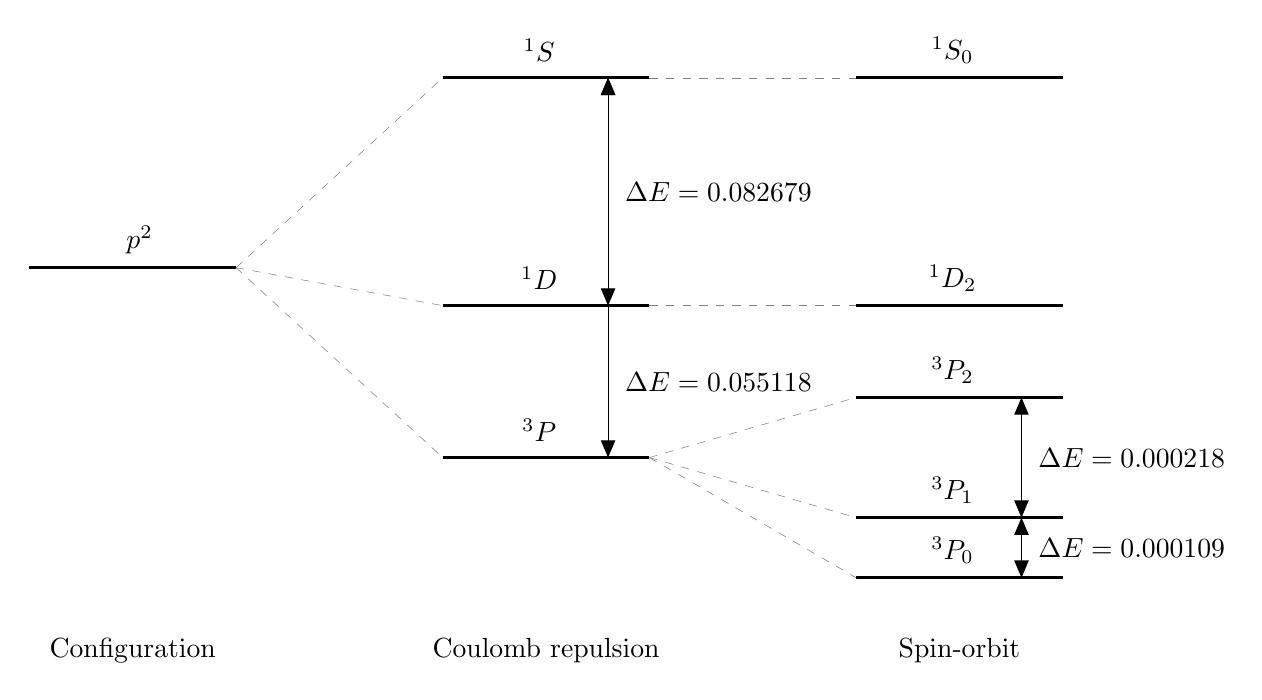
\begin{tikzpicture}[scale=0.175]
\newcommand{\LA}{0}
\newcommand{\RA}{15}
\newcommand{\LB}{30}
\newcommand{\RB}{45}
\newcommand{\LC}{60}
\newcommand{\RC}{75}
\newcommand{\EA}{13.7797}
\newcommand{\EBa}{27.5594}
\newcommand{\EBb}{11.0236}
\newcommand{\EBc}{0}
\newcommand{\ECa}{27.5594}
\newcommand{\ECb}{11.0236}
\newcommand{\ECc}{ 4.36}
\newcommand{\ECd}{-4.36}
\newcommand{\ECe}{-8.72}
%
\draw[very thick] (\LA,\EA) -- (\RA,\EA);
%
\draw[very thick] (\LB,\EBa) -- (\RB,\EBa);
\draw[very thick] (\LB,\EBb) -- (\RB,\EBb);
\draw[very thick] (\LB,\EBc) -- (\RB,\EBc);
%
\draw[very thick] (\LC,\ECa) -- (\RC,\ECa);
\draw[very thick] (\LC,\ECb) -- (\RC,\ECb);
\draw[very thick] (\LC,\ECc) -- (\RC,\ECc);
\draw[very thick] (\LC,\ECd) -- (\RC,\ECd);
\draw[very thick] (\LC,\ECe) -- (\RC,\ECe);
%
\node at (\LA+8,\EA+2) {$p^2$};
\node at (\LB+7,\EBa+2) {$^1S$};
\node at (\LB+7,\EBb+2) {$^1D$};
\node at (\LB+7,\EBc+2) {$^3P$};
\node at (\LC+7,\ECa+2) {$^1S_0$};
\node at (\LC+7,\ECb+2) {$^1D_2$};
\node at (\LC+7,\ECc+2) {$^3P_2$};
\node at (\LC+7,\ECd+2) {$^3P_1$};
\node at (\LC+7,\ECe+2) {$^3P_0$};
%
\draw[very thin, gray, dashed] (\RA,\EA) -- (\LB,\EBa);
\draw[very thin, gray, dashed] (\RA,\EA) -- (\LB,\EBb);
\draw[very thin, gray, dashed] (\RA,\EA) -- (\LB,\EBc);
%
\draw[very thin, gray, dashed] (\RB,\EBa) -- (\LC,\ECa);
\draw[very thin, gray, dashed] (\RB,\EBb) -- (\LC,\ECb);
\draw[very thin, gray, dashed] (\RB,\EBc) -- (\LC,\ECc);
\draw[very thin, gray, dashed] (\RB,\EBc) -- (\LC,\ECd);
\draw[very thin, gray, dashed] (\RB,\EBc) -- (\LC,\ECe);
%
\draw[triangle 45-triangle 45] (\LB+12,\EBa) -- (\LB+12,\EBb);
\draw[triangle 45-triangle 45] (\LB+12,\EBa) -- (\LB+12,\EBc);
\draw[triangle 45-triangle 45] (\LC+12,\ECc) -- (\LC+12,\ECd);
\draw[triangle 45-triangle 45] (\LC+12,\ECd) -- (\LC+12,\ECe);
%
\node at (\RB+5,19.2915) {$\Delta E = 0.082679$};
\node at (\RB+5,5.5118) {$\Delta E = 0.055118$};
\node at (\RC+5,0) {$\Delta E = 0.000218$};
\node at (\RC+5,-6.54) {$\Delta E = 0.000109$};
%
\node at (\LA+7.5,-14) {Configuration};
\node at (\LB+7.5,-14) {Coulomb repulsion};
\node at (\LC+7.5,-14) {Spin-orbit};
\end{tikzpicture}
\end{center}
\caption{Energy splitting (Coulomb repulsion plus spin-orbit interaction)
of the $p^2$ configuration of a carbon atom. Energies are given in units of Hartree (a.u.).
The spin-orbit splitting is magnified for a better plotting. (see Fig.~\ref{fig:cvspb}
for realistic scale.)}
\label{fig:p2splitSO}
\end{figure}

The spin-orbit splitting in Fig.~\ref{fig:p2splitSO} is magnified for a better plotting.
The actual splitting is rather tiny (remember the $1/c^2$ factor). But I want to
emphasize that there are two issues about the spin-orbit splitting, namely,
the ``scale'' and the ``shape''. This can be seen from Eqn.~(\ref{eq:ESO}).
The part
\begin{equation*}
[J(J+1)-L(L+1)-S(S+1)]
\end{equation*}
leads to the splitting ``shape'', which is determined by the multiplet term $^{2S+1}L$.
While the other part
\begin{equation*}
A(nl,LS)
\end{equation*}
controls the ``scale'' of the splitting.
We have seen that $A(nl,LS)$ can be separated into $X(nl)$ and $M(LS)$. For a
given multiplet term, $M(LS)$ is fixed. The final term that governs the scale is
\begin{equation*}
X(nl) = \Bra{nl}\xi(r)\Ket{nl} 
\end{equation*}
which is the coupling strength constant. For a not-so-heavy atom, $X(nl)$ is usually
weak (see Eqn.(\ref{eq:Xcarbon}) for a carbon atom). We can safely simplify
the spin-orbit interaction within a multiplet term and obtain surprisingly
accurate energies. But for a heavy atom, like uranium,
this spin-orbit coupling constant becomes strong due to the deep radial potential.
If the order of the spin-orbit splitting reaches the order of the multiplet
energy splitting, our ``spin-orbit within multiplet terms'' may no longer be
a good approximation. In this case, we should consider the spin-orbit interactions
within the entire shell and diagonalize the complete Hamiltonian.

\section{Spin-orbit coupling within the entire shell}
By saying ``within entire shell'', it means to solve the problem in the complete basis
of a given configuration, say, $p^2$,
\begin{center}
\vspace{-0.5em}
\begin{tabular}{|c|c|c|}
\hline
$\bullet$ & $\bullet$ & $\phantom{\bullet}$ \\ \hline
 &  &  \\
\hline
\end{tabular}
\begin{tabular}{|c|c|c|}
\hline
$\bullet$ & $\phantom{\bullet}$ & $\bullet$ \\ \hline
 &  &  \\
\hline
\end{tabular}
\begin{tabular}{|c|c|c|}
\hline
$\bullet$ & $\phantom{\bullet}$ & $\phantom{\bullet}$ \\ \hline
$\bullet$ &  &  \\
\hline
\end{tabular}
\begin{tabular}{|c|c|c|}
\hline
$\bullet$ & $\phantom{\bullet}$ & $\phantom{\bullet}$ \\ \hline
 & $\bullet$ &  \\
\hline
\end{tabular}
\begin{tabular}{|c|c|c|}
\hline
$\bullet$ & $\phantom{\bullet}$ & $\phantom{\bullet}$ \\ \hline
 &  & $\bullet$ \\
\hline
\end{tabular} \\
\vspace{0.5em}
\begin{tabular}{|c|c|c|}
\hline
$\phantom{\bullet}$ & $\bullet$ & $\bullet$ \\ \hline
 &  &  \\
\hline
\end{tabular}
\begin{tabular}{|c|c|c|}
\hline
$\phantom{\bullet}$ & $\bullet$ & $\phantom{\bullet}$ \\ \hline
$\bullet$ &  &  \\
\hline
\end{tabular}
\begin{tabular}{|c|c|c|}
\hline
$\phantom{\bullet}$ & $\bullet$ & $\phantom{\bullet}$ \\ \hline
 & $\bullet$ &  \\
\hline
\end{tabular}
\begin{tabular}{|c|c|c|}
\hline
$\phantom{\bullet}$ & $\bullet$ & $\phantom{\bullet}$ \\ \hline
 &  & $\bullet$ \\
\hline
\end{tabular}
\begin{tabular}{|c|c|c|}
\hline
$\phantom{\bullet}$ & $\phantom{\bullet}$ & $\bullet$ \\ \hline
$\bullet$ &  &  \\
\hline
\end{tabular} \\
\vspace{0.5em}
\begin{tabular}{|c|c|c|}
\hline
$\phantom{\bullet}$ & $\phantom{\bullet}$ & $\bullet$ \\ \hline
 & $\bullet$ &  \\
\hline
\end{tabular}
\begin{tabular}{|c|c|c|}
\hline
$\phantom{\bullet}$ & $\phantom{\bullet}$ & $\bullet$ \\ \hline
 &  & $\bullet$ \\
\hline
\end{tabular}
\begin{tabular}{|c|c|c|}
\hline
$\phantom{\bullet}$ & $\phantom{\bullet}$ & $\phantom{\bullet}$ \\ \hline
$\bullet$ & $\bullet$ &  \\
\hline
\end{tabular}
\begin{tabular}{|c|c|c|}
\hline
$\phantom{\bullet}$ & $\phantom{\bullet}$ & $\phantom{\bullet}$ \\ \hline
$\bullet$ &  & $\bullet$ \\
\hline
\end{tabular}
\begin{tabular}{|c|c|c|}
\hline
$\phantom{\bullet}$ & $\phantom{\bullet}$ & $\phantom{\bullet}$ \\ \hline
 & $\bullet$ & $\bullet$ \\
\hline
\end{tabular}
\end{center}
%
We have previously used the same basis when solving the Coulomb repulsion problem.
Since we have the basis already, the remaining task is to set up the matrix
representation of the spin-orbit Hamiltonian in our basis.
To construct the matrix representation, the first step is to reformulate the Hamiltonian
\begin{equation}
H_\text{SO} = \sum_{i=1}^N \xi(r_i) \boldsymbol{\ell}_i\cdot\vec{s}_i
\end{equation}
into second quantization,
\begin{equation} \label{eq:SO2nd}
H_\text{SO} = \sum_{\alpha,\beta} V_{\alpha\beta} c_\alpha^\dagger c_\beta
\end{equation}
where,
\begin{align*}
\alpha & = \{n_1,\,l_1,\,m_1,\,\sigma_1\} \\
\beta  & = \{n_2,\,l_2,\,m_2,\,\sigma_2\}
\end{align*}
enumerate all possible quantum states of electrons. Here we consider only
interactions within the same shell, so we restrict $n_1l_1=n_2l_2=nl$.
If you still remember, we devoted an entire chapter
calculating the Coulomb repulsion matrix element $U_{\alpha\beta\gamma\delta}$
since it was extremely complicated.
However, today, our spin-orbit matrix element
\begin{equation}
V_{\alpha\beta} = \Bra{\alpha} \xi(r) \boldsymbol{\ell}\cdot\vec{s} \Ket{\beta}
\end{equation}
can be calculated with zero difficulty.
This spin-orbit matrix element can be split into a radial dependent part
and an angular dependent part
\begin{equation}
V_{\alpha\beta} = \Bra{nl} \xi(r) \Ket{nl} \Bra{m_1\sigma_1} \boldsymbol{\ell}\cdot\vec{s} \Ket{m_2\sigma_2}
\end{equation}
%
The radial part $\Bra{nl}\xi(r)\Ket{nl}$ is identical to $X(nl)$
which we have discussed in Eqn.~(\ref{eq:Xnlint}). And the angular part,
\begin{align} \label{eq:AngularSO}
\Bra{m_1\sigma_1} \boldsymbol{\ell}\cdot\vec{s} \Ket{m_2\sigma_2}
& = \Bra{m_1\sigma_1} \ell_x s_x + \ell_y s_y + \ell_z s_z \Ket{m_2\sigma_2} \nonumber \\
& = \Bra{m_1\sigma_1} \frac{1}{2}\ell_+ s_- + \frac{1}{2}\ell_- s_+ + \ell_z s_z \Ket{m_2\sigma_2} \nonumber \\
& = \phantom{+} \frac{1}{2}\sqrt{(l+m_2+1)(l-m_2)\left(\frac{1}{2}+\sigma_2\right)\left(\frac{1}{2}-\sigma_2+1\right)} \Braket{m_1\sigma_1|m_2+1,\sigma_2-1} \nonumber \\
& \phantom{=}\, + \frac{1}{2}\sqrt{(l+m_2)(l-m_2+1)\left(\frac{1}{2}+\sigma_2+1\right)\left(\frac{1}{2}-\sigma_2\right)} \Braket{m_1\sigma_1|m_2-1,\sigma_2+1} \nonumber \\
& \phantom{=}\, + m_2\sigma_2\Braket{m_1\sigma_1|m_2\sigma_2}
\end{align}
can be computed easily with the orthonormality of angular wave functions,
\begin{equation}
\Braket{m_1\sigma_1|m_2\sigma_2} = \delta_{m_1m_2}\delta_{\sigma_1\sigma_2}
\end{equation}

Setting up the spin-orbit Hamiltonian is simpler than setting up the Coulomb
repulsion Hamiltonian since we have only $\alpha$ and $\beta$ indices
\begin{equation} \label{eq:Hsoij}
\Bra{i} H_\text{SO} \Ket{j} = 
\Bra{i} \sum_{\alpha,\beta} V_{\alpha\beta} c_\alpha^\dag c_\beta \Ket{j}
\end{equation}
%
Hence, the algorithm is also simpler with less for loops (comparing with Algorithm~\ref{alg:Huij}).
\begin{algorithm}[h!]
\caption{Set up Hamiltonian}\label{alg:Hsoij}
\begin{algorithmic}[1]
\Function{Hamiltonian}{$basis$}
\State $dim \gets basis.dim$
\For {$i \gets 0$ to $dim$}
\State $conf_i \gets basis.conf[i]$
\ForAll {$\alpha$}
\If {\Call{isBit}{$\alpha$, $conf_i$}}
\State $conf_\alpha \gets$ \Call{clearBit}{$\alpha$, $conf_i$}
\ForAll {$\beta$}
\If {\Call{!isBit}{$\beta$, $conf_\alpha$}}
\State $conf_\beta \gets$ \Call{setBit}{$\beta$, $conf_\alpha$}
\State $conf_j \gets conf_\beta$
\State $j \gets basis.index[conf_j]$
\State $H_\text{SO}[i,j] \gets H_\text{SO}[i,j] + fsign*V_{\alpha\beta}$
\EndIf
\EndFor
\EndIf
\EndFor
\EndFor
\State \Return $H_\text{SO}$
\EndFunction
\end{algorithmic}
\end{algorithm}

If we diagonalize $H_\text{SO}$ directly, we would obtain the eigen-energies
of the pure spin-orbit interaction. To include both Coulomb repulsion and spin-orbit coupling,
we should diagonalize (numerically) the sum $(H_U+H_\text{SO})$.
For not-so-heavy atoms, like carbon, the resulting eigen-energies are surprisingly close
to the eigen-energies we obtained from the ``within multiplet terms'' approximation, which
is pretty remarkable, since the solutions from two different approaches agree each other.
However, for heavy atoms, there is a large discrepancy between those two solutions.

For heavy atoms, the deep potential leads to large values in the derivative $dV/dr$.
Hence, the spin-orbit coupling constant $\Bra{nl}\xi(r)\Ket{nl}$ is large. For
strong spin-orbit interactions, the order of energy splitting can reach the order
of the Coulomb repulsion splitting.
In this case the approximation using spin-orbit coupling within multiplet terms
are no longer appropriate.

This can be clearly demonstrated by a comparison between a carbon (C) and a lead (Pb)
atom, which are from the same group with the same open shell configuration $p^2$.
Table~\ref{table:cvspb} tabulated the numerical energies of spin-orbit interactions
within multiplet terms and within entire shell.

\begin{table}[h!]
\caption{Comparison of open shell spin-orbit energies within multiplet
terms and within entire shell for a carbon atom and a lead atom.
Energies are given in units of Hartree (a.u.).}
\label{table:cvspb}
\begin{center}
\begin{tabular}{ c | c | c | c | c | c }
  \hline
 Elem & Orbital & \begin{tabular}[t]{@{}c@{}}Energy within\\multiplet terms\\($\times$degeneracy)\end{tabular} &
 \begin{tabular}[t]{@{}c@{}}Energy within\\entire shell\\($\times$degeneracy)\end{tabular} & Abs Error & Rel Error \\ \hline \hline
    C & $2p^2$  & 0.612081 ($\times 1$) & 0.612081 ($\times 1$) & 0.000000 & 0.000000 \\
      &         & 0.529402 ($\times 5$) & 0.529403 ($\times 5$) & 0.000001 & 0.000002 \\
      &         & 0.474393 ($\times 5$) & 0.474392 ($\times 5$) & 0.000001 & 0.000002 \\
      &         & 0.474175 ($\times 3$) & 0.474175 ($\times 3$) & 0.000000 & 0.000000 \\
      &         & 0.474066 ($\times 1$) & 0.474065 ($\times 1$) & 0.000001 & 0.000002 \\ \hline
   Pb & $6p^2$  & 0.323500 ($\times 1$) & 0.335963 ($\times 1$) & 0.012463 & 0.037096 \\
      &         & 0.272826 ($\times 5$) & 0.284981 ($\times 5$) & 0.012155 & 0.042652 \\
      &         & 0.252988 ($\times 5$) & 0.240833 ($\times 5$) & 0.012155 & 0.050471 \\
      &         & 0.225100 ($\times 3$) & 0.225100 ($\times 3$) & 0.000000 & 0.000000 \\
      &         & 0.211156 ($\times 1$) & 0.198693 ($\times 1$) & 0.012463 & 0.062725 \\
  \hline  
\end{tabular}
\end{center}
\end{table}

The discrepancy can be seen more easily from the spectrum plot in Fig.~\ref{fig:cvspb}.
The spin-orbit splitting within multiplet terms and within
the entire shell are plotted in the 3rd and 4th column of the plot, respectively.
It is difficult to resolve the spin-orbit splitting in the carbon atom plot, since the
energy differences are so tiny. But this tiny splitting gives a good approximation
when considering spin-orbit coupling within multiplet terms. On the other hand,
the amplitude of spin-orbit splitting in the lead atom reaches the amplitude of Coulomb
repulsion splitting. In this case, the energies from the ``within multiplet terms''
approximation do not match the (more accurate) full shell diagonalization.

\begin{figure}
\centering
\subfloat[][Carbon (C)]{
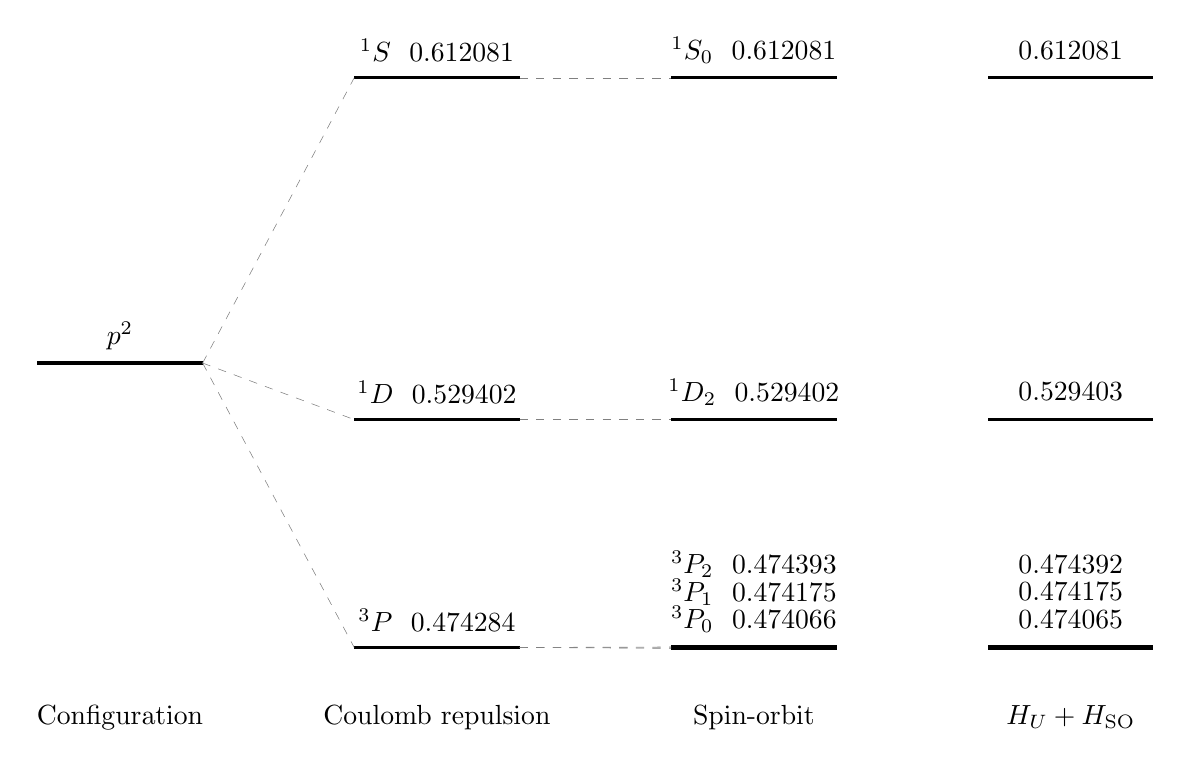
\begin{tikzpicture}[scale=0.175]
\newcommand{\LA}{0}
\newcommand{\RA}{12}
\newcommand{\LB}{23}
\newcommand{\RB}{35}
\newcommand{\LC}{46}
\newcommand{\RC}{58}
\newcommand{\LD}{69}
\newcommand{\RD}{81}
\newcommand{\EA}{13.8016*1.5}
\newcommand{\EBa}{27.6032*1.5}
\newcommand{\EBb}{11.0674*1.5}
\newcommand{\EBc}{0.0438*1.5}
\newcommand{\ECa}{27.6032*1.5}
\newcommand{\ECb}{11.0674*1.5}
\newcommand{\ECc}{0.0656*1.5}
\newcommand{\ECd}{0.0220*1.5}
\newcommand{\ECe}{0.0002*1.5}
\newcommand{\EDa}{27.6032*1.5}
\newcommand{\EDb}{11.0676*1.5}
\newcommand{\EDc}{0.0658*1.5}
\newcommand{\EDd}{0.0220*1.5}
\newcommand{\EDe}{0.0000*1.5}
%
\draw[very thick] (\LA,\EA) -- (\RA,\EA);
%
\draw[very thick] (\LB,\EBa) -- (\RB,\EBa);
\draw[very thick] (\LB,\EBb) -- (\RB,\EBb);
\draw[very thick] (\LB,\EBc) -- (\RB,\EBc);
%
\draw[very thick] (\LC,\ECa) -- (\RC,\ECa);
\draw[very thick] (\LC,\ECb) -- (\RC,\ECb);
\draw[very thick] (\LC,\ECc) -- (\RC,\ECc);
\draw[very thick] (\LC,\ECd) -- (\RC,\ECd);
\draw[very thick] (\LC,\ECe) -- (\RC,\ECe);
%
\draw[very thick] (\LD,\EDa) -- (\RD,\EDa);
\draw[very thick] (\LD,\EDb) -- (\RD,\EDb);
\draw[very thick] (\LD,\EDc) -- (\RD,\EDc);
\draw[very thick] (\LD,\EDd) -- (\RD,\EDd);
\draw[very thick] (\LD,\EDe) -- (\RD,\EDe);
%
\draw[very thin, gray, dashed] (\RA,\EA) -- (\LB,\EBa);
\draw[very thin, gray, dashed] (\RA,\EA) -- (\LB,\EBb);
\draw[very thin, gray, dashed] (\RA,\EA) -- (\LB,\EBc);
%
\draw[very thin, gray, dashed] (\RB,\EBa) -- (\LC,\ECa);
\draw[very thin, gray, dashed] (\RB,\EBb) -- (\LC,\ECb);
\draw[very thin, gray, dashed] (\RB,\EBc) -- (\LC,\ECc);
\draw[very thin, gray, dashed] (\RB,\EBc) -- (\LC,\ECd);
\draw[very thin, gray, dashed] (\RB,\EBc) -- (\LC,\ECe);
%
\node at (\LA+6,\EA+2) {$p^2$};
\node at (\LB+6,\EBa+2) {$^1S\ $ 0.612081};
\node at (\LB+6,\EBb+2) {$^1D\ $ 0.529402};
\node at (\LB+6,\EBc+2) {$^3P\ $ 0.474284};
\node at (\LC+6,\ECa+2) {$^1S_0\ $ 0.612081};
\node at (\LC+6,\ECb+2) {$^1D_2\ $ 0.529402};
\node at (\LC+6,\ECc+6) {$^3P_2\ $ 0.474393};
\node at (\LC+6,\ECc+4) {$^3P_1\ $ 0.474175};
\node at (\LC+6,\ECc+2) {$^3P_0\ $ 0.474066};
\node at (\LD+6,\EDa+2) {0.612081};
\node at (\LD+6,\EDb+2) {0.529403};
\node at (\LD+6,\EDc+6) {0.474392};
\node at (\LD+6,\EDc+4) {0.474175};
\node at (\LD+6,\EDc+2) {0.474065};
%
\node at (\LA+6,-5) {Configuration};
\node at (\LB+6,-5) {Coulomb repulsion};
\node at (\LC+6,-5) {Spin-orbit};
\node at (\LD+6,-5) {$H_U+H_\text{SO}$};
\end{tikzpicture}
\label{fig:c}} \\
\subfloat[][Lead (Pb)]{
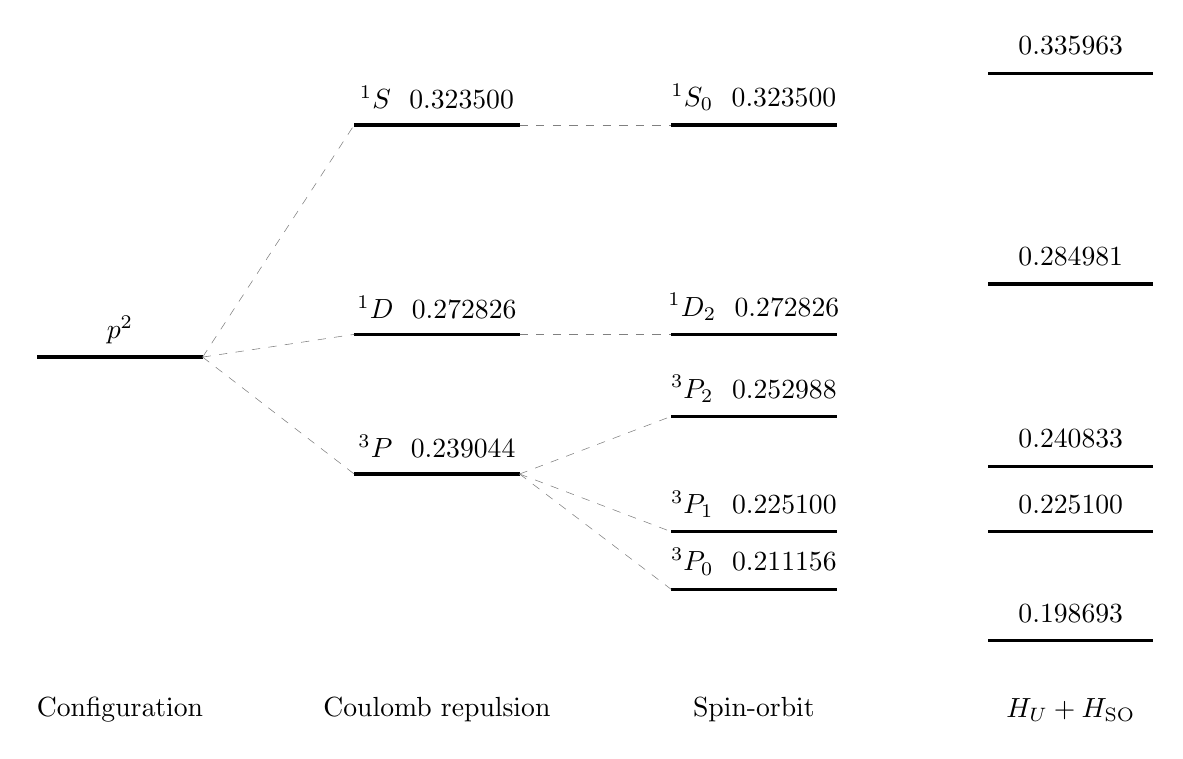
\begin{tikzpicture}[scale=0.175]
\newcommand{\LA}{0}
\newcommand{\RA}{12}
\newcommand{\LB}{23}
\newcommand{\RB}{35}
\newcommand{\LC}{46}
\newcommand{\RC}{58}
\newcommand{\LD}{69}
\newcommand{\RD}{81}
\newcommand{\EA}{13.7270*1.5}
\newcommand{\EBa}{24.9614*1.5}
\newcommand{\EBb}{14.8266*1.5}
\newcommand{\EBc}{ 8.0702*1.5}
\newcommand{\ECa}{24.9614*1.5}
\newcommand{\ECb}{14.8266*1.5}
\newcommand{\ECc}{10.8590*1.5}
\newcommand{\ECd}{ 5.2814*1.5}
\newcommand{\ECe}{ 2.4926*1.5}
\newcommand{\EDa}{27.4540*1.5}
\newcommand{\EDb}{17.2576*1.5}
\newcommand{\EDc}{ 8.4280*1.5}
\newcommand{\EDd}{ 5.2814*1.5}
\newcommand{\EDe}{ 0.0000*1.5}
%
\draw[very thick] (\LA,\EA) -- (\RA,\EA);
%
\draw[very thick] (\LB,\EBa) -- (\RB,\EBa);
\draw[very thick] (\LB,\EBb) -- (\RB,\EBb);
\draw[very thick] (\LB,\EBc) -- (\RB,\EBc);
%
\draw[very thick] (\LC,\ECa) -- (\RC,\ECa);
\draw[very thick] (\LC,\ECb) -- (\RC,\ECb);
\draw[very thick] (\LC,\ECc) -- (\RC,\ECc);
\draw[very thick] (\LC,\ECd) -- (\RC,\ECd);
\draw[very thick] (\LC,\ECe) -- (\RC,\ECe);
%
\draw[very thick] (\LD,\EDa) -- (\RD,\EDa);
\draw[very thick] (\LD,\EDb) -- (\RD,\EDb);
\draw[very thick] (\LD,\EDc) -- (\RD,\EDc);
\draw[very thick] (\LD,\EDd) -- (\RD,\EDd);
\draw[very thick] (\LD,\EDe) -- (\RD,\EDe);
%
\draw[very thin, gray, dashed] (\RA,\EA) -- (\LB,\EBa);
\draw[very thin, gray, dashed] (\RA,\EA) -- (\LB,\EBb);
\draw[very thin, gray, dashed] (\RA,\EA) -- (\LB,\EBc);
%
\draw[very thin, gray, dashed] (\RB,\EBa) -- (\LC,\ECa);
\draw[very thin, gray, dashed] (\RB,\EBb) -- (\LC,\ECb);
\draw[very thin, gray, dashed] (\RB,\EBc) -- (\LC,\ECc);
\draw[very thin, gray, dashed] (\RB,\EBc) -- (\LC,\ECd);
\draw[very thin, gray, dashed] (\RB,\EBc) -- (\LC,\ECe);
%
\node at (\LA+6,\EA+2) {$p^2$};
\node at (\LB+6,\EBa+2) {$^1S\ $ 0.323500};
\node at (\LB+6,\EBb+2) {$^1D\ $ 0.272826};
\node at (\LB+6,\EBc+2) {$^3P\ $ 0.239044};
\node at (\LC+6,\ECa+2) {$^1S_0\ $ 0.323500};
\node at (\LC+6,\ECb+2) {$^1D_2\ $ 0.272826};
\node at (\LC+6,\ECc+2) {$^3P_2\ $ 0.252988};
\node at (\LC+6,\ECd+2) {$^3P_1\ $ 0.225100};
\node at (\LC+6,\ECe+2) {$^3P_0\ $ 0.211156};
\node at (\LD+6,\EDa+2) {0.335963};
\node at (\LD+6,\EDb+2) {0.284981};
\node at (\LD+6,\EDc+2) {0.240833};
\node at (\LD+6,\EDd+2) {0.225100};
\node at (\LD+6,\EDe+2) {0.198693};
%
\node at (\LA+6,-5) {Configuration};
\node at (\LB+6,-5) {Coulomb repulsion};
\node at (\LC+6,-5) {Spin-orbit};
\node at (\LD+6,-5) {$H_U+H_\text{SO}$};
\end{tikzpicture}
\label{fig:pb}}
\caption{Comparison of open shell energy splitting between a ``light'' atom carbon (C)
and a ``heavy'' atom lead (Pb). Energies are given in units of Hartree (a.u.).
From left to right, 1st column: electronic configuration;
2nd column: Coulomb repulsion energy splitting; 3rd column: spin-orbit interaction
within multiplet terms; 4th column: eigen-energies of the Hamiltonian $(H_U+H_\text{SO})$.
Spin-orbit interaction within multiplet terms are good approximations for ``light'' atoms
but not for ``heavy'' atoms.}
\label{fig:cvspb}
\end{figure}

In the 4th column in Fig.~\ref{fig:cvspb}, we labeled each energy level by their numerical
values. But we didn't put a label like $^{2S+1}L$ or $^{2S+1}L_J$. This is because
when we consider the eigen-energies from the sum $(H_U+H_\text{SO})$, the energy levels are mixed
with contributions from different angular momenta $L$ and $S$. We can no longer
label each energy level as purely $^{2S+1}L$ or $^{2S+1}L_J$. Nevertheless, from the plot,
we do see some strong correspondence between the multiplet terms and the energy levels
from $(H_U+H_\text{SO})$. This correspondence can be calculated from the overlap between
the eigen-vectors of multiplet terms and the eigen-vectors of $(H_U+H_\text{SO})$, which
is known as the character of eigen-vectors.

For a multiplet term $^{2S+1}L$ (with seniority number $W$ if necessary), we have eigen-vectors
$\Ket{L,M_L,S,M_S}$ with $M_L=L,\ldots,-L$ and $M_S=S,\ldots,-S$. Those vectors span
a ``small space'' of this specific multiplet term. Now, suppose we have an
eigen-vector $\Ket{v}$ of $(H_U+H_\text{SO})$ from our numerical diagonalization.
To check if this eigen-vector $\Ket{v}$ lives inside this ``small space'',
we compute the character
\begin{equation} \label{eq:char}
\boxed{
\lambda = \sum_{M_L,M_S} \big|\Braket{L,M_L,S,M_S|v}\big|^2
}
\end{equation}
%
If $\Ket{v}$ lives completely in the space spanned by $\Ket{L,M_L,S,M_S}$,
we shall get $\lambda=1$. On the contrary, if $\Ket{v}$ is completely off,
we will get $\lambda=0$. However, in our problem, this $\Ket{v}$ is often
partly in one multiplet term and partly in the others. In this case we get
$0<\lambda<1$. The closer to 1, the stronger is the contribution from
this specific multiplet term.

Continuing with our discussion, we compute all characters for each numerical
eigen-vectors of $(H_U+H_\text{SO})$ within the three multiplet spaces $^1S$, $^1D$
and $^3P$. The characters are listed in Table~\ref{table:char}.

\begin{table}[h!]
\caption{Character of numerical eigen-vectors in different multiplet term spaces.
We highlight the main contribution using underlines.
Zero values are left as empty entries so that the structure can be seen clearly.}
\label{table:char}
\begin{center}
\begin{tabular}{ c | c | c | c | c | c }
  \hline
 Elem & Orbital & \begin{tabular}[t]{@{}c@{}}Energy within\\entire shell\\($\times$degeneracy)\end{tabular} &
 \begin{tabular}[t]{@{}c@{}}Character\\in $^1S$\end{tabular} &
 \begin{tabular}[t]{@{}c@{}}Character\\in $^1D$\end{tabular} &
 \begin{tabular}[t]{@{}c@{}}Character\\in $^3P$\end{tabular} \\ \hline \hline
    C & $2p^2$  & 0.612081 ($\times 1$) & \underline{0.999995} &          & 0.000005 \\
      &         & 0.529403 ($\times 5$) &          & \underline{0.999992} & 0.000008 \\
      &         & 0.474392 ($\times 5$) &          & 0.000008 & \underline{0.999992} \\
      &         & 0.474175 ($\times 3$) &          &          & \underline{1.000000} \\
      &         & 0.474065 ($\times 1$) & 0.000005 &          & \underline{0.999995} \\ \hline
   Pb & $6p^2$  & 0.335963 ($\times 1$) & \underline{0.909208} &          & 0.090792 \\
      &         & 0.284981 ($\times 5$) &          & \underline{0.724683} & 0.275317 \\
      &         & 0.240833 ($\times 5$) &          & 0.275317 & \underline{0.724683} \\
      &         & 0.225100 ($\times 3$) &          &          & \underline{1.000000} \\
      &         & 0.198693 ($\times 1$) & 0.090792 &          & \underline{0.909208} \\
  \hline
\end{tabular}
\end{center}
\end{table}

If you watch carefully and compare Table~\ref{table:char}
with Fig.~\ref{fig:cvspb}, you will notice that the terms are
mixed if they have the same $J$. Maybe you also noticed the interesting ``1.000000''
which never mixes with the others. That is because the vectors are from the
term with a unique $J$.

This table of characters directly indicates how strongly
are the eigen-states mixed among different multiplet terms (different
angular momenta). It again evidenced that with spin-orbit effect,
the eigen-states in carbon (light atom) are slightly mixed with different multiplet terms,
but the eigen-states in lead (heavy atom) are strongly mixed with different multiplet terms.
I must point out that, the numerical diagonalization of $(H_U+H_\text{SO})$
can always give us a better estimation of the eigen-energies (because it uses
the complete basis in the open shell), which is especially important for heavy atoms.
Nevertheless, our construction of multiplet states and
the first order perturbation theory in spin-orbit coupling give us a very
important understanding of the problem and a deep insight into the physical system.


\chapter{Summary}

If your friend asks you, ``What is multiplet?'' A short answer is,
``Multiplets are the many-electron eigen-states in atoms.'' But probably
he won't be satisfied since he knows the name but doesn't really understand
the problem. Then you give him the following box and two electrons,
\begin{equation*}
\begin{array}{c|c|c|c|}
\multicolumn{1}{c}{} & \multicolumn{1}{c}{\phantom{,}1\phantom{,}} & \multicolumn{1}{c}{\phantom{,}0\phantom{,}} & \multicolumn{1}{c}{-1} \\ \cline{2-4}
\uparrow &  &  &  \\ \cline{2-4}
\downarrow &  &  &  \\
\cline{2-4}
\multicolumn{1}{c}{}
\end{array}
\quad \text{and} \quad
\bullet \ \bullet
\end{equation*}

\vspace{-1.5em}
and ask, ``Let's put these two electrons into this $p$ shell.
In which configuration do you think this system has the highest energy?''
(don't ask for the lowest one, since it can be known easily from
Hund's rule) If he complains there is no difference in the way of putting
electrons, then he is speaking mean-field language, which is exactly what
we assumed in our Chapter~\ref{ch:3}. Fortunately, your friend is convinced
that electrons with different orbital and spin angular momenta
do repel each other differently (you showed him the plots in
Appendix~\ref{app:A}). But still, he won't
recognize which configuration has the highest energy, because this is
not at all a trivial problem! If you are also curious for the answer, I put
it here directly: the state
\begin{equation*}
\frac{1}{\sqrt{3}}
\begin{array}{|c|c|c|}
\hline
 & \phantom{\bullet} & \bullet \\ \hline
\bullet &  &  \\
\hline
\end{array}
- \frac{1}{\sqrt{3}}
\begin{array}{|c|c|c|}
\hline
\phantom{\bullet} & \bullet & \phantom{\bullet} \\ \hline
 & \bullet &  \\
\hline
\end{array}
+ \frac{1}{\sqrt{3}}
\begin{array}{|c|c|c|}
\hline
\bullet & \phantom{\bullet} & \\ \hline
 &  & \bullet \\
\hline
\end{array}
\end{equation*}
is an eigen-state of the $p^2$ configuration with the highest eigen-energy,
and it corresponds to the $^1S$ multiplet
(you see, nobody could answer this easily).
The complete problem is worked out step by step in Chapter~\ref{ch:5}.
Finally, in addition to Coulomb repulsion, we also included
spin-orbit coupling in Chapter~\ref{ch:6}, where we see the multiplet
spectral lines further split into finer structures.
Our work can be extended by introducing the $jj$-coupling,
where we consider each electron's total angular momentum. We can also
introduce external crystal field (our present work are in the frame of isolated
atoms) to study how our multiplet states respond to different external potential fields.

In the very end I must advertise our simulation tool: all the discussions in
this thesis have been implemented on a web page. Programming codes are written
in JavaScript. You can run simulations of all atoms on the periodic table
directly in a modern browser (no installation,
no compilation, and no plug-in).
This simulation tool can be accessed via the link:
\begin{center}
\url{www.cond-mat.de/sims/multiplet}
\end{center}


\appendix
\chapter{How to draw spherical harmonics} \label{app:A}

\section{The spherical harmonics}
For the first time students encounter spherical harmonics, we are most likely
scared away by the complicated expressions and bizarre geometries of the plots.
Complaining,
\begin{quote}
``I can never understand these functions and crazy plots. It's all so complicated!''
\end{quote}

This is, however, always the case when we learn something new. Things usually look
incomprehensible until we understand them and set up a good friendship.

Spherical harmonics are the solutions of the angular equation in (\ref{eq:YEqn}):
\begin{equation} \label{eq:YEqnAppend}
\frac{1}{\sin{\theta}} \frac{\partial}{\partial \theta} \left( \sin{\theta} \frac{\partial Y}{\partial \theta} \right) + \frac{1}{\sin^2{\theta}} \frac{\partial^2 Y}{\partial \phi^2} = -l(l+1) Y
\end{equation}
%
The derivations are nicely discussed in Griffiths' book \cite{QM}. In this short appendix,
we are not going to repeat the derivations, but will emphasize another interesting
perspective: how to draw the spherical harmonics. Not only for impressing your friends,
but more importantly, once we understood how they are plotted,
we will get a direct feeling of spherical harmonics and essentially comprehend their meanings.

The spherical harmonics $Y_{lm}(\theta,\phi)$ (with $l=0,\ 1,\ \ldots$ and $m=-l,\ \ldots,\ l$),
are given by
\begin{equation} \label{eq:sphaAppend}
Y_{lm}(\theta,\phi) = \sqrt{\frac{2l+1}{4\pi}\frac{(l-m)!}{(l+m)!}} P_l^m(\cos{\theta}) e^{im\phi}
\end{equation}
The big square root in front is nothing but a normalization factor, simply a real number.
The exponential term in the end is called the phase, which never contributes when we
consider the modulus square $|Y_{lm}|^2$. Probably the most scaring term is $P_l^m$, the
associated Legendre polynomials. But don't worry, they can be computed very easily. The computation
routine is clearly provided by \emph{Numerical Recipes} \cite{NR}. To give a direct impression,
Table~\ref{table:Ylm} explicitly listed the first few spherical harmonics.

\begin{table}[h!]
\caption{The first few spherical harmonics $Y_{lm}(\theta,\phi)$.}
\label{table:Ylm}
\begin{equation*}
\renewcommand\arraystretch{2.2}
\begin{array}{|>{\displaystyle}r >{\displaystyle}r >{\displaystyle}l >{\displaystyle}l|}
  \hline
  Y_{0,\phantom{\pm}0} = & \sqrt{\frac{1}{4\pi}}      &                                 &  \\[0.4em] \hline
  Y_{1,\phantom{\pm}0} = & \sqrt{\frac{3}{4\pi}}      & \cos{\theta}                    &  \\
  Y_{1,\pm1}           = & \mp\sqrt{\frac{3}{8\pi}}   & \sin{\theta}                    & e^{\pm i\phi} \\[0.4em] \hline
  Y_{2,\phantom{\pm}0} = & \sqrt{\frac{5}{16\pi}}     & (3\cos^2{\theta}-1)             &  \\
  Y_{2,\pm1}           = & \mp\sqrt{\frac{15}{8\pi}}  & \sin{\theta}\cos{\theta}        & e^{\pm i\phi} \\
  Y_{2,\pm2}           = & \sqrt{\frac{15}{32\pi}}    & \sin^2{\theta}                  & e^{\pm 2i\phi} \\[0.4em] \hline
  Y_{3,\phantom{\pm}0} = & \sqrt{\frac{7}{16\pi}}     & (5\cos^3{\theta}-3\cos{\theta}) &  \\
  Y_{3,\pm1}           = & \mp\sqrt{\frac{21}{64\pi}} & \sin{\theta}(5\cos^2{\theta}-1) & e^{\pm i\phi} \\
  Y_{3,\pm2}           = & \sqrt{\frac{105}{32\pi}}   & \sin^2{\theta}\cos{\theta}      & e^{\pm 2i\phi} \\
  Y_{3,\pm3}           = & \mp\sqrt{\frac{35}{64\pi}} & \sin^3{\theta}                  & e^{\pm 3i\phi} \\[0.4em]
  \hline
\end{array}
\end{equation*}
\end{table}

\section{Plotting in spherical coordinates}
Perhaps the most common and easiest way to make a plot is to plot in the Cartesian coordinate system.
Just like how we plotted our radial wave functions $u_{nl}(r)$. We took the $x$-axis representing
our spacial distance $r$ and $y$-axis representing our wave functions $u_{nl}$
\begin{equation} \label{eq:cartesian}
  \begin{cases}
  x \gets r \\
  y \gets u_{nl}
  \end{cases}
\end{equation}

However, for our angular wave functions, namely the spherical harmonics $Y_{lm}(\theta,\phi)$, it is
more natural to plot them in a spherical coordinate system, since it is where they are
defined. Now the mapping is the following,
\begin{equation} \label{eq:spherical}
  \begin{cases}
  r \gets Y_{lm} \\
  \theta \gets \theta \\
  \phi \gets \phi
  \end{cases}
\end{equation}

The important message is that we use the radius to represent the
amplitude of spherical harmonics. The functions listed in
Table~\ref{table:Ylm} are good enough for us to make a couple of
beautiful plots. For simplicity, we would like
to restrict the azimuthal angle $\phi$ to 0,
that is, we plot in the $xz$-plane. So now we have only one variable $\theta$.
To make the plots, we first define our grid in $\theta$
\begin{equation} \label{eq:thetaGrid}
\left\{ \theta_{\text{min}} = 0;\quad \theta_{\text{max}} = 2\pi;\quad \Delta \theta = \frac{\pi}{12}; \right\}
\end{equation}
To get started, let's plot the simplest function $Y_{00}$,

For $\theta=0\,\,\,$, we have $r=\sqrt{\frac{1}{4\pi}}$;\newline
For $\theta=\frac{\pi}{12}$, we have $r=\sqrt{\frac{1}{4\pi}}$;\newline
For $\theta=\frac{2\pi}{12}$, we have $r=\sqrt{\frac{1}{4\pi}}$;\newline
\ldots \newline
For $\theta=2\pi$, we have $r=\sqrt{\frac{1}{4\pi}}$.

If we plot these data points and connect them, we get a circle! (Fig.~\ref{fig:Y00})
\begin{figure}[h!]
\centering
  \includegraphics[width=0.36\textwidth,height=0.33\textwidth]{Y00}
  \caption{$Y_{00}(\theta,\phi)$ in the $xz$-plane.}
  \label{fig:Y00}
\end{figure}

$Y_{00}$ was simple enough. Let's try a more exciting one, $Y_{10}$,

For $\theta=0\,\,\,\,\,$, we have $\,\,r \approx 0.4886$;\newline
For $\theta=\frac{\pi}{12}\,\,$, we have $\,\,r \approx 0.4720$;\newline
\ldots \newline
For $\theta=\frac{7\pi}{12}\,\,$, we have $\boxed{r \approx -0.1265}$;\newline
\ldots \newline
For $\theta=\frac{23\pi}{12}$, we have $\,\,r \approx 0.4720$;\newline
For $\theta=2\pi\,\,$, we have $\,\,r \approx 0.4886$.

Wait! how do we plot a negative radius? Hum... we really can only plot the
absolute value. To indicate the different signs, let's use two different colors.
We use red color for positive $Y_{10}$ and blue color for negative $Y_{10}$.
Now we plot the data points and connect them. We get a red-blue colored plot in Fig.~\ref{fig:Y10}
\begin{figure}[h!]
\centering
  \includegraphics[width=0.36\textwidth,height=0.33\textwidth]{Y10}
  \caption{$Y_{10}(\theta,\phi)$ in the $xz$-plane.}
  \label{fig:Y10}
\end{figure}

The color of the plot doesn't contribute much into the physical meaning.
Never ever misunderstand them as positive or negative charges (or whatever). The physical
meaning is represented by the modulus square of the wave function $|Y_{lm}|^2$,
which is the probability density of finding an electron.
It doesn't really matter which color ($\pm$ sign) it is.

Previously we restricted our azimuthal angle to 0. It wouldn't be too difficult
to extend our discussion for arbitrary $\phi$. When we consider a non-zero $\phi$,
we may have the situation that $Y_{lm}$ is a complex number. But we simply
plot the modulus of the complex number, so it won't be a problem. Nevertheless,
if we want to indicate the phase of the complex number (just like for indicating the $\pm$ sign),
we can do some color mapping to make a fancy plot.
To get an idea how it works, we take the function $Y_{1,-1}$ as an example.
This time, we restrict our inclination angle $\theta$ to $\frac{\pi}{2}$, that is,
we plot in the $xy$-plane. Now we have freedom in $\phi$.
\begin{equation} \label{eq:phiGrid}
\left\{ \phi_{\text{min}} = 0;\quad \phi_{\text{max}} = 2\pi;\quad \Delta \phi = \frac{\pi}{12}; \right\}
\end{equation}
For $\phi=0\,\,\,$, we have $r \approx 0.3455 e^{\phantom{-}0.0000i}$;\newline
For $\phi=\frac{\pi}{12}$, we have $r \approx 0.3455 e^{-0.2618i}$;\newline
For $\phi=\frac{2\pi}{12}$, we have $r \approx 0.3455 e^{-0.5236i}$;\newline
\ldots \newline
For $\phi=2\pi$, we have $r \approx 0.3455 e^{-6.2832i}$.

We plot the modulus of the complex numbers as the radius. And we map the
colors according to the phase angles of the complex numbers,
which is the angle formed by the real and imaginary parts on
the complex plane. The choice of colors is arbitrary, but it is good to have some
continuously interpolated colors to represent the continuous phase angles. (Fig.~\ref{fig:Yphi})
\vspace{-0.5em}
\begin{figure}[h!]
\centering
  \includegraphics[width=0.36\textwidth,height=0.33\textwidth]{Yphi}
  \caption{$Y_{1,-1}(\theta,\phi)$ in the $xy$-plane.}
  \label{fig:Yphi}
\end{figure}

We have basically introduced all the essential ideas for plotting spherical
harmonics. All that remains is to implement (or use) a 3D visualization program
to visualize the $(r,\theta,\phi)$ data. Writing a 3D visualization program
involves some computer graphics knowledge, such as the coordinate transformations
and shading programs. I have implemented a program using the WebGL technology,
which can be run directly in a modern browser. I summarize some nice plots generated
by WebGL in Table~\ref{table:pureYlm}, which are the functions listed in Table~\ref{table:Ylm}.

\section{Linear combinations of spherical harmonics}
The spherical harmonics $Y_{lm}$ (called pure harmonics)
are solutions from Eqn.~(\ref{eq:YEqnAppend}).
Consequently, their linear combinations (with the same $l$) are also valid solutions.
Actually, you can take any crazy combinations to make some crazy plots.
But there are a handful of pre-defined linear combinations, which are
typically useful for chemists. Those pre-defined
combinations are called real harmonics. Because those
combinations (by combining $\pm m$)
eliminate the imaginary parts and result in
functions which are in the real range. The first few real harmonics
are listed in Table~\ref{table:realHarm}. The corresponding plots
are also given in Table~\ref{table:realYlm}. You will see only two
colors, because there are only positive and negative real numbers!

\begin{table}[h!]
\caption{The first few real harmonics.}
\label{table:realHarm}
\vspace{1em}
\hspace{4em}
\begin{minipage}{0.4\textwidth}
\begin{equation*}
\renewcommand\arraystretch{2.2}
\begin{array}{|>{\displaystyle}l >{\displaystyle}c >{\displaystyle}l|}
  \hline
  s               & = & Y_{0,0}                       \\[0.4em] \hline
  p_z             & = & Y_{1,0}                       \\
  p_x             & = & \sqrt{\frac{1}{2}}\phantom{i}(Y_{1,-1}-Y_{1,1})  \\
  p_y             & = & \sqrt{\frac{1}{2}}i(Y_{1,-1}+Y_{1,1}) \\[0.4em] \hline
  d_{3z^2-1}      & = & Y_{2,0}                       \\
  d_{xz}          & = & \sqrt{\frac{1}{2}}\phantom{i}(Y_{2,-1}-Y_{2,1})  \\
  d_{yz}          & = & \sqrt{\frac{1}{2}}i(Y_{2,-1}+Y_{2,1}) \\
  d_{x^2-y^2}     & = & \sqrt{\frac{1}{2}}\phantom{i}(Y_{2,-2}+Y_{2,2})  \\
  d_{xy}          & = & \sqrt{\frac{1}{2}}i(Y_{2,-2}-Y_{2,2}) \\[0.4em]
  \hline
\end{array}
\end{equation*}
\end{minipage}
\begin{minipage}{0.4\textwidth}
\begin{equation*}
\renewcommand\arraystretch{2.2}
\begin{array}{|>{\displaystyle}l >{\displaystyle}c >{\displaystyle}l|}
  \hline
  f_{z(5z^2-3)}   & = & Y_{3,0}                       \\
  f_{x(5z^2-1)}   & = & \sqrt{\frac{1}{2}}\phantom{i}(Y_{3,-1}-Y_{3,1})  \\
  f_{y(5z^2-1)}   & = & \sqrt{\frac{1}{2}}i(Y_{3,-1}+Y_{3,1}) \\
  f_{z(x^2-y^2)}  & = & \sqrt{\frac{1}{2}}\phantom{i}(Y_{3,-2}+Y_{3,2})  \\
  f_{xyz}         & = & \sqrt{\frac{1}{2}}i(Y_{3,-2}-Y_{3,2}) \\
  f_{x(x^2-3y^2)} & = & \sqrt{\frac{1}{2}}\phantom{i}(Y_{3,-3}-Y_{3,3})  \\
  f_{y(3x^2-y^2)} & = & \sqrt{\frac{1}{2}}i(Y_{3,-3}+Y_{3,3}) \\[0.4em]
  \hline
\end{array}
\end{equation*}
\end{minipage}
\end{table}

\clearpage
\begin{table}
\begin{center}
\small
\rotatebox{-90}{
\begin{minipage}{\textheight}
\caption{The first few pure spherical harmonics.}
\label{table:pureYlm}
\makebox[1.1\textheight]{
\begin{tabular}{c c c c c c c}
& & & \includegraphics[width=0.14\textwidth,trim={0 3cm 0 -2cm},clip]{00} & & & \\
& & & $l=0,\;m=0$ & & & \\
& & \includegraphics[width=0.14\textwidth,trim={0 3cm 0 -2cm},clip]{1m1} & \includegraphics[width=0.14\textwidth,trim={0 3cm 0 -2cm},clip]{10} & \includegraphics[width=0.14\textwidth,trim={0 3cm 0 -2cm},clip]{1p1} & & \\
& & $l=1,\;m=-1$ & $l=1,\;m=0$ & $l=1,\;m=1$ & & \\
& \includegraphics[width=0.14\textwidth,trim={0 3cm 0 -2cm},clip]{2m2} & \includegraphics[width=0.14\textwidth,trim={0 3cm 0 -2cm},clip]{2m1} & \includegraphics[width=0.14\textwidth,trim={0 3cm 0 -2cm},clip]{20} & \includegraphics[width=0.14\textwidth,trim={0 3cm 0 -2cm},clip]{2p1} & \includegraphics[width=0.14\textwidth,trim={0 3cm 0 -2cm},clip]{2p2} & \\
& $l=2,\;m=-2$ & $l=2,\;m=-1$ & $l=2,\;m=0$ & $l=2,\;m=1$ & $l=2,\;m=2$ & \\
\includegraphics[width=0.14\textwidth,trim={0 3cm 0 -2cm},clip]{3m3} & \includegraphics[width=0.14\textwidth,trim={0 3cm 0 -2cm},clip]{3m2} & \includegraphics[width=0.14\textwidth,trim={0 3cm 0 -2cm},clip]{3m1} & \includegraphics[width=0.14\textwidth,trim={0 3cm 0 -2cm},clip]{30} & \includegraphics[width=0.14\textwidth,trim={0 3cm 0 -2cm},clip]{3p1} & \includegraphics[width=0.14\textwidth,trim={0 3cm 0 -2cm},clip]{3p2} & \includegraphics[width=0.14\textwidth,trim={0 3cm 0 -2cm},clip]{3p3} \\ 
$l=3,\;m=-3$ & $l=3,\;m=-2$ & $l=3,\;m=-1$ & $l=3,\;m=0$ & $l=3,\;m=1$ & $l=3,\;m=2$ & $l=3,\;m=3$
\end{tabular}
}
\end{minipage}
}
\end{center}
\end{table}
\clearpage
\begin{table}
\begin{center}
\small
\rotatebox{-90}{
\begin{minipage}{\textheight}
\caption{The first few real spherical harmonics.}
\label{table:realYlm}
\makebox[1.1\textheight]{
\begin{tabular}{c c c c c c c}
& & & \includegraphics[width=0.14\textwidth,trim={0 3cm 0 -2cm},clip]{s} & & & \\
& & & $s$ & & & \\
& & \includegraphics[width=0.14\textwidth,trim={0 3cm 0 -2cm},clip]{px} & \includegraphics[width=0.14\textwidth,trim={0 3cm 0 -2cm},clip]{pz} & \includegraphics[width=0.14\textwidth,trim={0 3cm 0 -2cm},clip]{py} & & \\
& & $p_x$ & $p_z$ & $p_y$ & & \\
& \includegraphics[width=0.14\textwidth,trim={0 3cm 0 -2cm},clip]{dxxyy} & \includegraphics[width=0.14\textwidth,trim={0 3cm 0 -2cm},clip]{dxz} & \includegraphics[width=0.14\textwidth,trim={0 3cm 0 -2cm},clip]{d3zz1} & \includegraphics[width=0.14\textwidth,trim={0 3cm 0 -2cm},clip]{dyz} & \includegraphics[width=0.14\textwidth,trim={0 3cm 0 -2cm},clip]{dxy} & \\
& $d_{x^2-y^2}$ & $d_{xz}$ & $d_{3z^2-1}$ & $d_{yz}$ & $d_{xy}$ & \\
\includegraphics[width=0.14\textwidth,trim={0 3cm 0 -2cm},clip]{fxxx3yy} & \includegraphics[width=0.14\textwidth,trim={0 3cm 0 -2cm},clip]{fzxxyy} & \includegraphics[width=0.14\textwidth,trim={0 3cm 0 -2cm},clip]{fx5zz1} & \includegraphics[width=0.14\textwidth,trim={0 3cm 0 -2cm},clip]{fz5zz3} & \includegraphics[width=0.14\textwidth,trim={0 3cm 0 -2cm},clip]{fy5zz1} & \includegraphics[width=0.14\textwidth,trim={0 3cm 0 -2cm},clip]{fxyz} & \includegraphics[width=0.14\textwidth,trim={0 3cm 0 -2cm},clip]{fy3xxyy} \\
$f_{x(x^2-3y^2)}$ & $f_{z(x^2-y^2)}$ & $f_{x(5z^2-1)}$ & $f_{z(5z^2-3)}$ & $f_{y(5z^2-1)}$ & $f_{xyz}$ & $f_{y(3x^2-y^2)}$ 
\end{tabular}
}
\end{minipage}
}
\end{center}
\end{table}
\clearpage


\chapter{Second quantization} \label{app:B}

\section{A different formalism but the same physics}
In real space, electrons are described as wave functions.
Because electrons are fermions, their anti-symmetric wave functions are
formulated as Slater determinants \cite{GBK}. (as a remark, a many-electron wave function
$\Psi(\vec{r}_1,\ldots,\vec{r}_N)$ is in general a linear combination
of Slater determinants. Meanwhile, we are ignoring spin to simplify our notations.)
\begin{equation} \label{eq:slaterdeterm}
\Phi_{\alpha_1\cdots\alpha_N}(\vec{r}_1,\ldots,\vec{r}_N) = \frac{1}{\sqrt{N!}}
\begin{vmatrix}
\varphi_{\alpha_1}(\vec{r}_1) & \varphi_{\alpha_2}(\vec{r}_1) & \cdots & \varphi_{\alpha_N}(\vec{r}_1) \\
\varphi_{\alpha_1}(\vec{r}_2) & \varphi_{\alpha_2}(\vec{r}_2) & \cdots & \varphi_{\alpha_N}(\vec{r}_2) \\
\vdots & \vdots & \ddots & \vdots \\
\varphi_{\alpha_1}(\vec{r}_N) & \varphi_{\alpha_2}(\vec{r}_N) & \cdots & \varphi_{\alpha_N}(\vec{r}_N)
\end{vmatrix}
\end{equation}
%
For a one-electron wave function, Eqn.~(\ref{eq:slaterdeterm}) is trivial:
\begin{equation}
\Phi_\alpha(\vec{r}_1) = \varphi_\alpha(\vec{r}_1)
\end{equation}
%
For a two-electron wave function, Eqn.~(\ref{eq:slaterdeterm}) reads:
\begin{equation}
\Phi_{\alpha\beta}(\vec{r}_1,\vec{r}_2) = \frac{1}{\sqrt{2}}(\varphi_\alpha(\vec{r}_1)\varphi_\beta(\vec{r}_2)
- \varphi_\beta(\vec{r}_1)\varphi_\alpha(\vec{r}_2))
\end{equation}
%
For a three-electron wave function, Eqn.~(\ref{eq:slaterdeterm}) becomes:
\begin{align} \label{eq:3SD}
\Phi_{\alpha\beta\gamma}(\vec{r}_1,\vec{r}_2,\vec{r}_3) = & {} \frac{1}{\sqrt{6}}
\Big(\phantom{-}\varphi_\alpha(\vec{r}_1)\varphi_\beta(\vec{r}_2)\varphi_\gamma(\vec{r}_3)
+ \varphi_\gamma(\vec{r}_1)\varphi_\alpha(\vec{r}_2)\varphi_\beta(\vec{r}_3)
+ \varphi_\beta(\vec{r}_1)\varphi_\gamma(\vec{r}_2)\varphi_\alpha(\vec{r}_3) \nonumber \\
& {} \phantom{\frac{1}{\sqrt{6}}(} {-\varphi_\gamma(\vec{r}_1)}\varphi_\beta(\vec{r}_2)\varphi_\alpha(\vec{r}_3)
- \varphi_\beta(\vec{r}_1)\varphi_\alpha(\vec{r}_2)\varphi_\gamma(\vec{r}_3)
- \varphi_\alpha(\vec{r}_1)\varphi_\gamma(\vec{r}_2)\varphi_\beta(\vec{r}_3) \Big)
\end{align}
%
I wouldn't intend to write the four-electron wave function since it will be super long.
This trouble is actually caused by working with real space.
Since we need to label $\vec{r}_1, \vec{r}_2, \ldots, \vec{r}_N$ for different
degrees of freedom, we must use the Slater determinant to ensure the anti-symmetry
property of the wave function, which unfortunately makes the expression very complicated.
We can get rid of this difficulty if not working with real space. To specify an electron
in state $\alpha$, instead of $\varphi_\alpha(\vec{r}_1)$, we write
\begin{equation*}
\Ket{\alpha}
\end{equation*}
%
which is known as the Dirac state \cite{QM}. Now, for a two-electron state, we write
\begin{equation*}
\Ket{\alpha, \beta}
\end{equation*}
%
But how do we ensure the anti-symmetry of this two-electron state?
\begin{equation}
\Ket{\alpha, \beta} = -\Ket{\beta, \alpha}
\end{equation}
%
Previously, when working with real space, this was ensured by the
Slater determinant. Now, this anti-symmetry will be taken care by the
second quantization operators.\footnote{The order of the operators indicates
we create $\alpha$ first and $\beta$ second. Hence we write
$c_\beta^\dagger c_\alpha^\dagger \Ket{0} = \Ket{\alpha,\beta}$.}
\begin{equation}
\Ket{\alpha, \beta} = c_\beta^\dagger c_\alpha^\dagger \Ket{0}
\end{equation}
%
These lovely operators have the property that if they change order, they produce
a minus sign (the fermi-sign).
\begin{equation}
\Ket{\alpha, \beta} = c_\beta^\dagger c_\alpha^\dagger \Ket{0} =
- c_\alpha^\dagger c_\beta^\dagger \Ket{0} = -\Ket{\beta, \alpha}
\end{equation}
%
Surprisingly, the anti-symmetry property is automatically ensured!
With second quantization, many-electron states could
be written out with no pain.

For a one-electron state,
\begin{equation}
\Ket{\alpha} = c_\alpha^\dagger \Ket{0}
\end{equation}
%
For a two-electron state,
\begin{equation}
\Ket{\alpha,\beta} = c_\beta^\dagger c_\alpha^\dagger \Ket{0}
\end{equation}
%
For a three-electron state,
\begin{equation}
\Ket{\alpha,\beta,\gamma} = c_\gamma^\dagger c_\beta^\dagger c_\alpha^\dagger \Ket{0}
\end{equation}
%
We do not need to worry about the anti-symmetry, because it is taken care by
those operators automatically. This is the idea of second quantization.
It must be pointed out, second quantization does not involve any new physics.
Sometimes this name is misleading that people tend to ask, ``Wait, what
was the first quantization? Well, if the quantization of electron was the first,
what is the second one?'' No, no! Nothing is further quantized. Second quantization
is just a novel ``algebra'' that simplifies the formalism of many-body problems.

Suppose we have a state
\begin{equation}
\Ket{\text{example}} = \frac{1}{\sqrt{6}} \left( c_\alpha^\dagger c_\beta^\dagger c_\gamma^\dagger +2c_\delta^\dagger c_\epsilon^\dagger c_\zeta^\dagger +c_\eta^\dagger c_\theta^\dagger c_\iota^\dagger \right)|0\rangle
\end{equation}
%
which is a linear combination of three different Slater determinants.
It would be horrible to express it in real space (repeat Eqn.~(\ref{eq:3SD})
three times). Second quantization provides us a very convenient way
to handle many-body states.

\section{Creation and annihilation operators}
We start from the vacuum state $\Ket{0}$, which is a state with no electron.
Although without electron, it is defined to be normalized $\Braket{0|0}=1$.
Next, we introduce the creation operator $c_\alpha^\dagger$.
If $c_\alpha^\dagger$ applies on a vacuum state,
it creates one electron with state $\alpha$,
\begin{equation}
c_\alpha^\dagger \Ket{0} = \Ket{\alpha}
\end{equation}
%
``Hum? Create an electron out of vacuum?'' No, no! We are not going to
set up a lab to create electrons out of photons or whatever. This is purely
an algebra. By saying ``create'', it is from a mathematics point of view,
not a physical process. Similarly, we have an electron annihilation operator
$c_\alpha$. If $c_\alpha$ applies on a vacuum state, it returns zero
\begin{equation}
c_\alpha \Ket{0} = 0
\end{equation}
%
Previously, we claimed that the creation operators anti-commute:
$c_\alpha^\dagger c_\beta^\dagger = -c_\beta^\dagger c_\alpha^\dagger$.
This is one of the definitions in second quantization. Now, the commutation
relation between a creator and an annihilator is defined as
\begin{equation}
c_\alpha c_\beta^\dagger = \Braket{\alpha|\beta} -c_\beta^\dagger c_\alpha
\end{equation}
%
When working with orthonormal basis states, $\Braket{\alpha|\beta}=\delta_{\alpha\beta}$.
Let's see what happens if $c_\alpha$ applies on a state $\Ket{\alpha}$
\begin{equation}
c_\alpha \Ket{\alpha} = c_\alpha c_\alpha^\dagger \Ket{0}
= (1 - c_\alpha^\dagger c_\alpha) \Ket{0}
= \Ket{0} - c_\alpha^\dagger \underbrace{c_\alpha \Ket{0}}_{=0} = \Ket{0}
\end{equation}
%
As the name suggests, it removes one electron from $\Ket{\alpha}$ and
brings back the vacuum state. But this is purely an algebraic consequence,
not a definition.
The entire definition of second quantization
algebra are summarized in Table~\ref{table:secondQ}.
%
\begin{table}[h!]
\caption{The definition of second quantization algebra.}
\label{table:secondQ}
\begin{equation*}
\renewcommand\arraystretch{1.8}
\begin{array}{|>{\displaystyle}r >{\displaystyle}c >{\displaystyle}l|}
  \hline
  \Braket{0|0} & = & 1 \\
  c_\alpha\Ket{0} & = & 0 \\
  \{c_\alpha^\dagger, c_\beta^\dagger\} & = & 0 \\
  \{c_\alpha, c_\beta\} & = & 0 \\
  \{c_\alpha, c_\beta^\dagger\} & = & \Braket{\alpha|\beta} \\[0.2em]
  \hline
\end{array}
\end{equation*}
\end{table}

where the anti-commutator,
\begin{equation}
\{A,B\} \equiv AB + BA
\end{equation}
%
Believe it or not, with simply five definitions,
Table~\ref{table:secondQ} defines the complete system which formulates
second quantization.

\section{The bridge between first and second quantization}
A two-electron Slater determinant in first quantization (real space),
\begin{equation*}
\frac{1}{\sqrt{2}}(\varphi_\alpha(\vec{r}_1)\varphi_\beta(\vec{r}_2)
- \varphi_\beta(\vec{r}_1)\varphi_\alpha(\vec{r}_2))
\end{equation*}
%
A two-electron Slater determinant in second quantization (configuration space),
\begin{equation*}
c_\beta^\dagger c_\alpha^\dagger \Ket{0}
\end{equation*}
%
However, these two are not the same:
\begin{equation} \label{eq:real2nd}
c_\beta^\dagger c_\alpha^\dagger \Ket{0} \ne
\frac{1}{\sqrt{2}}(\varphi_\alpha(\vec{r}_1)\varphi_\beta(\vec{r}_2)
- \varphi_\beta(\vec{r}_1)\varphi_\alpha(\vec{r}_2))
\end{equation}
%
A wave function is a wave function and a state is a state.
They describe the same Slater determinant, but one cannot put an equal sign in between.
To make the connection between real space and second quantization, we need some
special electron creators and annihilators (called field operators).
Although physically not possible,
algebraically we can ``create'' an electron in such a state that it is
exactly at position $\vec{r}$. We denote
$c_\vec{r}^\dagger \Ket{0} = \Ket{\vec{r}}$.\footnote{Because of the importance of
these special creators and annihilators, they get a name, field operators. A more
standard way to write field operators are $\hat{\Psi}(\vec{r})$ and
$\hat{\Psi}^\dagger(\vec{r})$ (see Reference \cite{GBK}). But I would like to 
stick with $c_\vec{r}$ and $c_\vec{r}^\dagger$ to simplify our notations.}
Suppose we have an $\Ket{\alpha}$ state which in real space corresponds
to wave function $\varphi_\alpha(\vec{r})$.
Considering $\varphi_\alpha(\vec{r})$ as an amplitude, $c_\alpha^\dagger$
and $c_\vec{r}^\dagger$ are (intuitively) related as
\begin{equation} \label{eq:cacr}
c_\alpha^\dagger = \int d^3r\,\varphi_\alpha(\vec{r}) c_\vec{r}^\dagger
\end{equation}
%
Conversely, if we have a complete(!) set of single electron wave
functions $\varphi_{\alpha_n}(\vec{r})$, we can expand the field operators
in terms of the corresponding creators and annihilators
\begin{equation} \label{eq:crca}
c_\vec{r}^\dagger = \sum_n \varphi_{\alpha_n}(\vec{r}) c_{\alpha_n}^\dagger
\end{equation}
%
Using Eqn.~(\ref{eq:cacr}), we find the anti-commutation relation
\begin{equation}
\{c_\vec{r}, c_\alpha^\dagger \} =
\int d^3r'\,\varphi_\alpha(\vec{r'}) \{c_\vec{r}, c_\vec{r'}^\dagger \} = \varphi_\alpha(\vec{r})
\end{equation}
which is such a golden relation that helps us bridge
second quantization to real space. For example,
a one-electron Slater determinant,
\begin{equation}
\Braket{\vec{r}_1|\alpha} = \Bra{0} c_{\vec{r}_1} c_{\alpha}^\dagger \Ket{0}
= \Bra{0} \varphi_{\alpha}(\vec{r}_1) - c_{\alpha}^\dagger c_{\vec{r}_1} \Ket{0}
= \varphi_{\alpha}(\vec{r}_1)
\end{equation}
Nice! We get back our wave function in real space. Next,
for a two-electron Slater determinant,
\begin{align}
\Braket{\vec{r}_2,\vec{r}_1|\alpha,\beta}
& = \Bra{0} c_{\vec{r}_1} c_{\vec{r}_2} c_{\beta}^\dagger c_{\alpha}^\dagger \Ket{0} \nonumber \\
& = \Bra{0} c_{\vec{r}_1} (\varphi_\beta(\vec{r_2}) - c_{\beta}^\dagger c_{\vec{r}_2}) c_{\alpha}^\dagger \Ket{0} \nonumber \\
& = \Bra{0} c_{\vec{r}_1} c_\alpha^\dagger \Ket{0} \varphi_\beta(\vec{r}_2) - \Bra{0} c_{\vec{r}_1} c_{\beta}^\dagger c_{\vec{r}_2} c_\alpha^\dagger \Ket{0} \nonumber \\
& = \varphi_\alpha(\vec{r}_1) \varphi_\beta(\vec{r}_2) - \varphi_\beta(\vec{r}_1) \varphi_\alpha(\vec{r}_2)
\end{align}
%
Impressive! Even the two-electron anti-symmetric wave function is automatically returned.
A proof by induction is nicely discussed in Reference \cite{GBK}. Here we quote
the conclusion, for an $N$-electron state, its real-space Slater determinant
representation is given by
\begin{equation} \label{eq:bridge}
\boxed{
\Phi_{\alpha_1\cdots\alpha_N}(\vec{r}_1,\ldots,\vec{r}_N)
= \frac{1}{\sqrt{N!}}
\Bra{0} c_{\vec{r}_1} c_{\vec{r}_2} \cdots c_{\vec{r}_N}
c_{\alpha_N}^\dagger \cdots c_{\alpha_2}^\dagger c_{\alpha_1}^\dagger \Ket{0}
}
\end{equation}
%
From our quantum mechanics lectures, we often see the relation,
\begin{equation}
\Braket{\alpha|\beta} = \int d^3r\, \conj{\varphi_\alpha}(\vec{r}) \varphi_\beta(\vec{r})
\end{equation}
This can also be shown using our field operators:
\begin{align}
\Braket{\alpha|\beta}
& = \Bra{0} c_\alpha c_\beta^\dagger \Ket{0}
 = \Bra{0} \int d^3r\, \conj{\varphi_\alpha}(\vec{r}) c_\vec{r} \varphi_\beta(\vec{r}) c_{\vec{r}}^\dagger \Ket{0} \nonumber \\
& = \int d^3r\, \conj{\varphi_\alpha}(\vec{r}) \varphi_\beta(\vec{r}) \underbrace{\Bra{0} c_\vec{r} c_{\vec{r}}^\dagger \Ket{0}}_{=1}
= \int d^3r\, \conj{\varphi_\alpha}(\vec{r}) \varphi_\beta(\vec{r})
\end{align}
Similarly, for the two electron case,
\begin{align}
\Braket{\alpha,\beta|\gamma,\delta}
& = \Bra{0} c_\beta c_\alpha c_\delta^\dagger c_\gamma^\dagger \Ket{0}
= \Bra{0} c_\alpha c_\beta c_\gamma^\dagger c_\delta^\dagger \Ket{0} \nonumber \\
& = \Bra{0} \int d^3r_1\, \conj{\varphi_\alpha}(\vec{r}_1) c_{\vec{r}_1} \varphi_\delta(\vec{r}_1) c_{\vec{r}_1}^\dagger
\int d^3r_2\, \conj{\varphi_\beta}(\vec{r}_2) c_{\vec{r}_2} \varphi_\gamma(\vec{r}_2) c_{\vec{r}_2}^\dagger \Ket{0} \nonumber \\
& = \int d^3r_1\int d^3r_2\, \conj{\varphi_\alpha}(\vec{r}_1) \conj{\varphi_\beta}(\vec{r}_2) \varphi_\gamma(\vec{r}_2) \varphi_\delta(\vec{r}_1) \underbrace{\Bra{0} c_{\vec{r}_1} c_{\vec{r}_1}^\dagger c_{\vec{r}_2} c_{\vec{r}_2}^\dagger \Ket{0}}_{=1}
\end{align}
Those lovely operators $c_{\vec{r}}$ and $c_{\vec{r}}^\dagger$ play a role
bridging first and second quantization. But they never appear explicitly
in either first or second quantization!

\section{Representation of $n$-body operators}
In Chapter~\ref{ch:4}, we were working with the Coulomb repulsion Hamiltonian,
\begin{equation} \label{eq:appHu}
H_U = \sum_{i<j}^N \frac{1}{|\vec{r}_i - \vec{r}_j|}
\end{equation}
which is a two-body operator.

In Chapter~\ref{ch:6}, we introduced the spin-orbit coupling Hamiltonian,
\begin{equation} \label{eq:appHso}
H_\text{SO} = \sum_{i=1}^N \xi(r_i) \boldsymbol{\ell}_i\cdot\vec{s}_i
\end{equation}
which is a one-body operator.

Eqn.~(\ref{eq:appHu}) and Eqn.~(\ref{eq:appHso}) are in the form of
the so called first quantization. They operate on real-space wave functions.
A second quantization many-body state is, however, not compatible with
those operators. A beautiful discussion (you must give a look)
of transforming real-space operators to second quantization operators
is given in \cite{GBK}. A key idea is to use the ``bridge'' in Eqn.~(\ref{eq:bridge}).
To avoid repeating the same content, I write down the results directly:

For the Coulomb repulsion Hamiltonian,
\begin{equation}
H_U = \frac{1}{2} \sum_{\alpha,\beta,\gamma,\delta} \Bra{\alpha,\beta} \frac{1}{|\vec{r}_1-\vec{r}_2|} \Ket{\gamma,\delta} c_\alpha^\dag c_\beta^\dag c_\gamma c_\delta
\end{equation}
which is given in Eqn.~(\ref{eq:U2nd}).

For the spin-orbit coupling Hamiltonian,
\begin{equation}
H_\text{SO} = \sum_{\alpha,\beta} \Bra{\alpha} \xi(r) \boldsymbol{\ell}\cdot\vec{s} \Ket{\beta} c_\alpha^\dagger c_\beta
\end{equation}
which is given in Eqn.~(\ref{eq:SO2nd}).

They are the Hamiltonians compatible with second quantization states.

\section{Electron-hole transformation}
In this section, we would like to restrict our discussion on atomic
shell basis states instead of general states.
In Eqn.~(\ref{eq:createorder}), we made a convention that for a
fully occupied shell, the electron creators
are arranged in the following way:
\vspace{-0.5em}
\begin{equation}
\begin{array}{c|c|c|c|}
\multicolumn{1}{c}{} & \multicolumn{1}{c}{\phantom{,}1\phantom{,}} & \multicolumn{1}{c}{\phantom{,}0\phantom{,}} & \multicolumn{1}{c}{-1} \\ \cline{2-4}
\uparrow & \bullet & \bullet & \bullet \\ \cline{2-4}
\downarrow & \bullet & \bullet & \bullet \\
\cline{2-4}
\multicolumn{1}{c}{}
\end{array} =
c_{-1\downarrow}^\dagger c_{0\downarrow}^\dagger c_{1\downarrow}^\dagger
c_{-1\uparrow}^\dagger c_{0\uparrow}^\dagger c_{1\uparrow}^\dagger
\Ket{0}
\end{equation}

\vspace{-2em}
Now we understand why it is important to make such a convention: the
convention is arbitrary, but once it is decided, it must remain
unchanged through the entire discussion, since changing the order of
electron creators involves fermi-signs ($\pm1$).

To motivate the topic of this section, let's
consider an almost-full shell, say, a $d^8$:
\vspace{-0.5em}
\begin{equation*}
\begin{array}{c|c|c|c|c|c|}
\multicolumn{1}{c}{} & \multicolumn{1}{c}{\phantom{,}2\phantom{,}} &
\multicolumn{1}{c}{\phantom{,}1\phantom{,}} & \multicolumn{1}{c}{\phantom{,}0\phantom{,}} &
\multicolumn{1}{c}{-1} & \multicolumn{1}{c}{-2} \\ \cline{2-6}
\uparrow & \bullet & \bullet & \bullet & \bullet &  \\ \cline{2-6}
\downarrow & \bullet & \bullet &  & \bullet & \bullet \\
\cline{2-6}
\end{array}
\end{equation*}
%
We would write it in terms of electron creation operators as
\begin{equation*}
c_{-2\downarrow}^\dagger c_{-1\downarrow}^\dagger c_{1\downarrow}^\dagger c_{2\downarrow}^\dagger
c_{-1\uparrow}^\dagger c_{0\uparrow}^\dagger c_{1\uparrow}^\dagger c_{2\uparrow}^\dagger
\Ket{0}
\end{equation*}
%
This becomes a bit cumbersome and not very readable (but of course
much simpler than its real-space form). We noticed that if we express
the same state in terms of the unoccupied sites, the expression will become
much shorter. What we need to do is to transform our ``electron algebra''
into a ``hole algebra''.
Let's start from the fully occupied $d$ shell
\begin{equation} \label{eq:full}
\Ket{\text{full}} = 
c_{-2\downarrow}^\dagger c_{-1\downarrow}^\dagger c_{0\downarrow}^\dagger c_{1\downarrow}^\dagger c_{2\downarrow}^\dagger
c_{-2\uparrow}^\dagger c_{-1\uparrow}^\dagger c_{0\uparrow}^\dagger c_{1\uparrow}^\dagger c_{2\uparrow}^\dagger
\Ket{0}
\end{equation}
%
Notice that a $\Ket{\text{full}}$ state also has $M_L=0$ and $M_S=0$.
From the hole's point of view, the $\Ket{\text{full}}$ state behaves like a
``vacuum'' state. Creating a hole at site ($-m,-\sigma$) on a $\Ket{\text{full}}$ state
leaves the system with momentum $M_L=m$ and $M_S=\sigma$.
Hence we could define our hole creation operator as
\begin{equation} \label{eq:simpdef}
h_{m\sigma}^\dagger = c_{-m,-\sigma}
\end{equation}
%
But this is not very convenient. Because what we really want is, for example,
\begin{equation} \label{eq:hfull}
\begin{array}{|c|c|c|c|c|}
\hline
\bullet & \bullet & \bullet & \bullet &  \\ \hline
\bullet & \bullet & \bullet & \bullet & \bullet \\
\hline
\end{array}
= h_{2\downarrow}^\dagger \Ket{\text{full}}
\end{equation}

\vspace{-1em}
However,
\begin{align}
\begin{array}{|c|c|c|c|c|}
\hline
\bullet & \bullet & \bullet & \bullet &  \\ \hline
\bullet & \bullet & \bullet & \bullet & \bullet \\
\hline
\end{array}
& = c_{-2\downarrow}^\dagger c_{-1\downarrow}^\dagger c_{0\downarrow}^\dagger c_{1\downarrow}^\dagger c_{2\downarrow}^\dagger
c_{-1\uparrow}^\dagger c_{0\uparrow}^\dagger c_{1\uparrow}^\dagger c_{2\uparrow}^\dagger
\Ket{0} \nonumber \\
& = c_{-2\downarrow}^\dagger c_{-1\downarrow}^\dagger c_{0\downarrow}^\dagger c_{1\downarrow}^\dagger c_{2\downarrow}^\dagger
\boxed{c_{-2\uparrow}} c_{-2\uparrow}^\dagger c_{-1\uparrow}^\dagger c_{0\uparrow}^\dagger c_{1\uparrow}^\dagger c_{2\uparrow}^\dagger
\Ket{0} \nonumber \\
& = (-1)^{5} \boxed{c_{-2\uparrow}}
\underbrace{c_{-2\downarrow}^\dagger c_{-1\downarrow}^\dagger c_{0\downarrow}^\dagger c_{1\downarrow}^\dagger c_{2\downarrow}^\dagger
c_{-2\uparrow}^\dagger c_{-1\uparrow}^\dagger c_{0\uparrow}^\dagger c_{1\uparrow}^\dagger c_{2\uparrow}^\dagger
\Ket{0}}_{\Ket{\text{full}}} \nonumber \\
& = - c_{-2\uparrow} \Ket{\text{full}} = - h_{2\downarrow}^\dagger \Ket{\text{full}}
\end{align}
%
If we really want to write as the way in Eqn.~(\ref{eq:hfull}),
we must absorb the fermi-sign into definition (\ref{eq:simpdef}).
According to our full shell definition, this fermi-sign has the following pattern
\begin{equation*}
\begin{array}{|c|}
\hline
- \\ \hline
+ \\
\hline
\end{array}
\quad
\begin{array}{|c|c|c|}
\hline
- & + & - \\ \hline
+ & - & + \\
\hline
\end{array}
\quad
\begin{array}{|c|c|c|c|c|}
\hline
- & + & - & + & - \\ \hline
+ & - & + & - & + \\
\hline
\end{array}
\quad
\begin{array}{|c|c|c|c|c|c|c|}
\hline
- & + & - & + & - & + & - \\ \hline
+ & - & + & - & + & - & + \\
\hline
\end{array}
\end{equation*}
%
Therefore, we define, (the definition is subject to how a $\Ket{\text{full}}$ is defined)
\begin{equation} \label{eq:ehtrans}
\boxed{
h_{m\sigma}^\dagger = (-1)^{l+m+\sigma-\frac{1}{2}} c_{-m,-\sigma}
}
\end{equation}
%
The next question is how to arrange these hole operators. Previously
we made a convention of ordering electron creators. Now we no longer
have this freedom to define new convention of ordering
hole creators. As a consequence from previous convention, the hole
creators should be ordered in the following way:
(notice that it is the same order of putting electrons)
\vspace{-0.5em}
\begin{equation}
\begin{array}{c|c|c|c|}
\multicolumn{1}{c}{} & \multicolumn{1}{c}{\phantom{,}1\phantom{,}} & \multicolumn{1}{c}{\phantom{,}0\phantom{,}} & \multicolumn{1}{c}{-1} \\ \cline{2-4}
\uparrow &  &  &  \\ \cline{2-4}
\downarrow &  &  &  \\
\cline{2-4}
\multicolumn{1}{c}{}
\end{array} =
h_{1\uparrow}^\dagger h_{0\uparrow}^\dagger h_{-1\uparrow}^\dagger
h_{1\downarrow}^\dagger h_{0\downarrow}^\dagger h_{-1\downarrow}^\dagger
\Ket{\text{full}}
\end{equation}

\vspace{-2em}
In general, an $N$-electron basis vector and a $(2(2l-1)-N)$-hole basis vector
are equivalent by the relation,
\begin{equation*}
\prod_{i=1}^N c_{m_i\sigma_i}^\dagger \Ket{0} =
\prod_{j=1}^{2(2l-1)-N} h_{m_j\sigma_j}^\dagger \Ket{\text{full}}
\end{equation*}
The indices $\{j\}$ run over the complement part of indices $\{i\}$,
for example,
\begin{equation}
\begin{array}{|c|c|c|c|c|}
\hline
i_1 & i_2 & i_3 & i_4 & j_1 \\ \hline
i_5 & i_6 & j_2 & i_7 & i_8 \\
\hline
\end{array}
\end{equation}
To show their equivalence,
\begin{equation}
\prod_{j=1}^{2(2l-1)-N} h_{m_j\sigma_j}^\dagger \Ket{\text{full}}
= \prod_{j=1}^{2(2l-1)-N} (-1)^{l+m_j+\sigma_j-\frac{1}{2}} c_{-m_j,-\sigma_j} \prod_{i=1}^{2(2l+1)} c_{m_i\sigma_i}^\dagger \Ket{0}
\end{equation}
But anti-commuting $c_{-m_j,-\sigma_j}$ into the full shell always cancels the
$(-1)^{l+m_j+\sigma_j-\frac{1}{2}}$ factor (that is how this factor is designed for).
After all anti-commutations, what left is,
\begin{equation}
\prod_{j=1}^{2(2l-1)-N} h_{m_j\sigma_j}^\dagger \Ket{\text{full}}
= \prod_{i=1}^N c_{m_i\sigma_i}^\dagger \Ket{0}
\end{equation}
%
We can verify that our example state
\begin{align}
\begin{array}{|c|c|c|c|c|}
\hline
\bullet & \bullet & \bullet & \bullet &  \\ \hline
\bullet & \bullet &  & \bullet & \bullet \\
\hline
\end{array}
& = h_{0\uparrow}^\dagger h_{2\downarrow}^\dagger \Ket{\text{full}}
= - c_{0\downarrow} c_{-2\uparrow} \Ket{\text{full}} \nonumber \\
& = - c_{0\downarrow} \boxed{c_{-2\uparrow}}
c_{-2\downarrow}^\dagger c_{-1\downarrow}^\dagger c_{0\downarrow}^\dagger c_{1\downarrow}^\dagger c_{2\downarrow}^\dagger
c_{-2\uparrow}^\dagger c_{-1\uparrow}^\dagger c_{0\uparrow}^\dagger c_{1\uparrow}^\dagger c_{2\uparrow}^\dagger
\Ket{0} \nonumber \\
& = (-1)^6 c_{0\downarrow}
c_{-2\downarrow}^\dagger c_{-1\downarrow}^\dagger c_{0\downarrow}^\dagger c_{1\downarrow}^\dagger c_{2\downarrow}^\dagger
\boxed{c_{-2\uparrow}} c_{-2\uparrow}^\dagger c_{-1\uparrow}^\dagger c_{0\uparrow}^\dagger c_{1\uparrow}^\dagger c_{2\uparrow}^\dagger
\Ket{0} \nonumber \\
& = (-1)^6 \boxed{c_{0\downarrow}}
c_{-2\downarrow}^\dagger c_{-1\downarrow}^\dagger c_{0\downarrow}^\dagger c_{1\downarrow}^\dagger c_{2\downarrow}^\dagger
c_{-1\uparrow}^\dagger c_{0\uparrow}^\dagger c_{1\uparrow}^\dagger c_{2\uparrow}^\dagger
\Ket{0} \nonumber \\
& = (-1)^8
c_{-2\downarrow}^\dagger c_{-1\downarrow}^\dagger \boxed{c_{0\downarrow}} c_{0\downarrow}^\dagger c_{1\downarrow}^\dagger c_{2\downarrow}^\dagger
c_{-1\uparrow}^\dagger c_{0\uparrow}^\dagger c_{1\uparrow}^\dagger c_{2\uparrow}^\dagger
\Ket{0} \nonumber \\
& =
c_{-2\downarrow}^\dagger c_{-1\downarrow}^\dagger c_{1\downarrow}^\dagger c_{2\downarrow}^\dagger
c_{-1\uparrow}^\dagger c_{0\uparrow}^\dagger c_{1\uparrow}^\dagger c_{2\uparrow}^\dagger
\Ket{0}
\end{align}
is indeed equivalent to the expression in terms of electron creators.

Eqn.~(\ref{eq:ehtrans}) is essentially the portal connecting the electron world with
the hole world. With this definition, we can investigate the properties of hole
operators. First of all, the $\Ket{\text{full}}$ state is normalized,
$\Braket{\text{full}|\text{full}}=1$. If we apply a hole annihilation operator
on it, according to Pauli exclusion principle, $h_{m\sigma}\Ket{\text{full}}=0$.
Now, we test the anti-commutation relation between hole operators.
\begin{align}
\{ h_{m_1\sigma_1}^\dagger, h_{m_2\sigma_2}^\dagger \}
& = (-1)^{2l+m_1+m_2+\sigma_1+\sigma_2-1} \{ c_{-m_1,-\sigma_1}, c_{-m_2,-\sigma_2} \} = 0 \\
\{ h_{m_1\sigma_1}, h_{m_2\sigma_2} \}
& = (-1)^{2l+m_1+m_2+\sigma_1+\sigma_2-1} \{ c_{-m_1,-\sigma_1}^\dagger, c_{-m_2,-\sigma_2}^\dagger \} = 0 \\
\{ h_{m_1\sigma_1}, h_{m_2\sigma_2}^\dagger \}
& = (-1)^{2l+m_1+m_2+\sigma_1+\sigma_2-1} \{ c_{-m_1,-\sigma_1}^\dagger, c_{-m_2,-\sigma_2} \} \nonumber \\
& = (-1)^{2l+m_1+m_2+\sigma_1+\sigma_2-1} \delta_{m_1m_2} \delta_{\sigma_1\sigma_2}
= \delta_{m_1m_2} \delta_{\sigma_1\sigma_2}
\end{align}
%
It turns out (not by definition), our hole operators behave exactly as electron
operators.
\begin{table}[h!]
\caption{Second quantization algebra from the hole's perspective.}
\label{table:secondQhole}
\begin{equation*}
\renewcommand\arraystretch{1.8}
\begin{array}{|>{\displaystyle}r >{\displaystyle}c >{\displaystyle}l|}
  \hline
  \Braket{\text{full}|\text{full}} & = & 1 \\
  h_{m\sigma}\Ket{\text{full}} & = & 0 \\
  \{h_{m_1\sigma_1}^\dagger, h_{m_2\sigma_2}^\dagger\} & = & 0 \\
  \{h_{m_1\sigma_1}, h_{m_2\sigma_2}\} & = & 0 \\
  \{h_{m_1\sigma_1}, h_{m_2\sigma_2}^\dagger\} & = & \delta_{m_1m_2} \delta_{\sigma_1\sigma_2} \\[0.2em]
  \hline
\end{array}
\end{equation*}
\end{table}




\backmatter{}

\chapter*{Acknowledgements}

I am heartily thankful to my supervisor, Prof.\ Dr.\ Erik Koch,
for his guidance, encouragement and support throughout my entire
thesis. He was always so patient to answer my frequent questions
and guided me to think and solve problems systematically.
I also would like to thank Dr.\ Hermann Ulm who promised me that
I can ask him any question. He helped me a lot in understanding
many detailed problems and gave me very strong encouragement through my thesis.
I am grateful to German Research School for Simulation Sciences for
providing me this great opportunity of doing my master thesis.
I am also thankful to Dr.\ Hunter Sims, Khaldoon Ghanem and Michael Baumg\"{a}rtel
for their many different helps during my thesis period.
In the end, I want to express my many thanks to Cica Gustiani, Rodrigo Canales
and Thu Hoai for our best memories studying and working together.


\begin{thebibliography}{99}
  \bibitem{QM} D.\ J.\ Griffiths: {\em Introduction to Quantum Mechanics}, Pearson Prentice Hall (2005).

  \bibitem{ES} R.\ M.\ Martin: {\em Electronic Structure}, Cambridge University Press (2004).
  
  \bibitem{KS} W.\ Kohn and L.\ J.\ Sham: {\em Self-Consistent Equations Including Exchange and Correlation Effects}, Physical Review A {\bf 140}, 1133 (1965).

  \bibitem{LDA} J.\ M.\ MacLaren, D.\ P.\ Clougherty, M.\ E.\ McHenry and M.\ M.\ Donovan: {\em Parameterised local spin density exchange-correlation energies and potentials for electronic structure calculations}, Computer Physics Communications {\bf 66}, 383--391 (1991).

  \bibitem{NIST} S.\ Kotochigova, Z.\ H.\ Levine, E.\ L.\ Shirley, M.\ D.\ Stiles and C.\ W.\ Clark: {\em Atomic Reference Data for Electronic Structure Calculations}, Physical Measurement Laboratory, NIST.\\ Link: \url{http://www.nist.gov/pml/data/dftdata/}
  
  \bibitem{WB} M.\ Weissbluth: {\em Atoms and Molecules}, Academic Press (1978).
  
  \bibitem{EM} D.\ J.\ Griffiths: {\em Introduction to Electrodynamics}, Prentice Hall (1999).
  
  \bibitem{CP} N.\ J.\ Giordano and H.\ Nakanishi: {\em Computational Physics}, Pearson Prentice Hall (2006).
  
  \bibitem{NR} W.\,H.\,Press, S.\,A.\,Teukolsky, W.\,T.\,Vetterling and B.\,P.\,Flannery: {\em Numerical Recipes in C}, Cambridge University Press (1992).

  \bibitem{MC} S.\ E.\ Koonin and D.\ C.\ Meredith: {\em Compututational Physics}, Westview Press (1990).
  
  \bibitem{RI} G.\ Racah: {\em Theory of Complex Spectra.~I}, Physical Review {\bf 61}, 186 (1942).

  \bibitem{RII} G.\ Racah: {\em Theory of Complex Spectra.~II}, Physical Review {\bf 62}, 438 (1942).
  
  \bibitem{RIII} G.\ Racah: {\em Theory of Complex Spectra.~III}, Physical Review {\bf 63}, 367 (1943).
  
  \bibitem{RIV} G.\ Racah: {\em Theory of Complex Spectra.~IV}, Physical Review {\bf 76}, 1352 (1949).
  
  \bibitem{YBK} E.\ Koch: {\em Exchange Mechanisms}, in \cite{YB}.
  
  \bibitem{GBK} E.\ Koch: {\em Many-Electron States}, in \cite{GB}.
  
  \bibitem{YBE} R.\ Eder: {\em Multiplets in Transition Metal Ions}, in \cite{YB}.
  
  \bibitem{YB} E.\ Pavarini, E.\ Koch, F.\ Anders and M.\ Jarrell (eds.): {\em Correlated Electrons: From Models to Materials}, Reihe Modeling and Simulation, Vol.\ 2, Forschungszentrum J\"{u}lich (2012).
  
  \bibitem{GB} E.\ Pavarini, E.\ Koch and U.\ Schollw\"{o}ck (eds.): {\em Emergent Phenomena in Correlated Matter}, Reihe Modeling and Simulation, Vol.\ 3, Forschungszentrum J\"{u}lich (2013).
\end{thebibliography}


\chapter*{Declaration of authorship}

I, \theauthor, hereby declare that I have created this work completely on my own and
used no other sources or tools than the ones listed, and that I have marked
any citations accordingly.

\begin{minipage}[c]{\textwidth}
    \vspace{2cm}
    \makebox[\textwidth][c]{
        \makebox[.6\textwidth][l] {\textrm{\theplace, \thedate}}
        \hfill
        \makebox[.4\textwidth][c] {\hrulefill}
        \hfill
    }
    \makebox[\textwidth][c]{
        \hfill
        \makebox[.6\textwidth][c] {}
        \emph{\theauthor}
        \hfill
    }
\end{minipage}


% Empty page at the end
\newpage
\thispagestyle{empty}
\mbox{}

\end{document}  
